\documentclass[twoside]{book}

% Packages required by doxygen
\usepackage{fixltx2e}
\usepackage{calc}
\usepackage{doxygen}
\usepackage[export]{adjustbox} % also loads graphicx
\usepackage{graphicx}
\usepackage[utf8]{inputenc}
\usepackage{makeidx}
\usepackage{multicol}
\usepackage{multirow}
\PassOptionsToPackage{warn}{textcomp}
\usepackage{textcomp}
\usepackage[nointegrals]{wasysym}
\usepackage[table]{xcolor}

% Font selection
\usepackage[T1]{fontenc}
\usepackage[scaled=.90]{helvet}
\usepackage{courier}
\usepackage{amssymb}
\usepackage{sectsty}
\renewcommand{\familydefault}{\sfdefault}
\allsectionsfont{%
  \fontseries{bc}\selectfont%
  \color{darkgray}%
}
\renewcommand{\DoxyLabelFont}{%
  \fontseries{bc}\selectfont%
  \color{darkgray}%
}
\newcommand{\+}{\discretionary{\mbox{\scriptsize$\hookleftarrow$}}{}{}}

% Page & text layout
\usepackage{geometry}
\geometry{%
  a4paper,%
  top=2.5cm,%
  bottom=2.5cm,%
  left=2.5cm,%
  right=2.5cm%
}
\tolerance=750
\hfuzz=15pt
\hbadness=750
\setlength{\emergencystretch}{15pt}
\setlength{\parindent}{0cm}
\setlength{\parskip}{3ex plus 2ex minus 2ex}
\makeatletter
\renewcommand{\paragraph}{%
  \@startsection{paragraph}{4}{0ex}{-1.0ex}{1.0ex}{%
    \normalfont\normalsize\bfseries\SS@parafont%
  }%
}
\renewcommand{\subparagraph}{%
  \@startsection{subparagraph}{5}{0ex}{-1.0ex}{1.0ex}{%
    \normalfont\normalsize\bfseries\SS@subparafont%
  }%
}
\makeatother

% Headers & footers
\usepackage{fancyhdr}
\pagestyle{fancyplain}
\fancyhead[LE]{\fancyplain{}{\bfseries\thepage}}
\fancyhead[CE]{\fancyplain{}{}}
\fancyhead[RE]{\fancyplain{}{\bfseries\leftmark}}
\fancyhead[LO]{\fancyplain{}{\bfseries\rightmark}}
\fancyhead[CO]{\fancyplain{}{}}
\fancyhead[RO]{\fancyplain{}{\bfseries\thepage}}
\fancyfoot[LE]{\fancyplain{}{}}
\fancyfoot[CE]{\fancyplain{}{}}
\fancyfoot[RE]{\fancyplain{}{\bfseries\scriptsize Generated by Doxygen }}
\fancyfoot[LO]{\fancyplain{}{\bfseries\scriptsize Generated by Doxygen }}
\fancyfoot[CO]{\fancyplain{}{}}
\fancyfoot[RO]{\fancyplain{}{}}
\renewcommand{\footrulewidth}{0.4pt}
\renewcommand{\chaptermark}[1]{%
  \markboth{#1}{}%
}
\renewcommand{\sectionmark}[1]{%
  \markright{\thesection\ #1}%
}

% Indices & bibliography
\usepackage{natbib}
\usepackage[titles]{tocloft}
\setcounter{tocdepth}{3}
\setcounter{secnumdepth}{5}
\makeindex

% Hyperlinks (required, but should be loaded last)
\usepackage{ifpdf}
\ifpdf
  \usepackage[pdftex,pagebackref=true]{hyperref}
\else
  \usepackage[ps2pdf,pagebackref=true]{hyperref}
\fi
\hypersetup{%
  colorlinks=true,%
  linkcolor=blue,%
  citecolor=blue,%
  unicode%
}

% Custom commands
\newcommand{\clearemptydoublepage}{%
  \newpage{\pagestyle{empty}\cleardoublepage}%
}

\usepackage{caption}
\captionsetup{labelsep=space,justification=centering,font={bf},singlelinecheck=off,skip=4pt,position=top}

%===== C O N T E N T S =====

\begin{document}

% Titlepage & ToC
\hypersetup{pageanchor=false,
             bookmarksnumbered=true,
             pdfencoding=unicode
            }
\pagenumbering{alph}
\begin{titlepage}
\vspace*{7cm}
\begin{center}%
{\Large Fear\+\_\+of\+\_\+ocean }\\
\vspace*{1cm}
{\large Generated by Doxygen 1.8.13}\\
\end{center}
\end{titlepage}
\clearemptydoublepage
\pagenumbering{roman}
\tableofcontents
\clearemptydoublepage
\pagenumbering{arabic}
\hypersetup{pageanchor=true}

%--- Begin generated contents ---
\chapter{Data Structure Index}
\section{Data Structures}
Here are the data structures with brief descriptions\+:\begin{DoxyCompactList}
\item\contentsline{section}{\hyperlink{structenigme}{enigme} }{\pageref{structenigme}}{}
\item\contentsline{section}{\hyperlink{structGameobject}{Gameobject} }{\pageref{structGameobject}}{}
\item\contentsline{section}{\hyperlink{structGestion}{Gestion} }{\pageref{structGestion}}{}
\item\contentsline{section}{\hyperlink{structHero}{Hero} }{\pageref{structHero}}{}
\item\contentsline{section}{\hyperlink{structInput}{Input} }{\pageref{structInput}}{}
\item\contentsline{section}{\hyperlink{structMap}{Map} }{\pageref{structMap}}{}
\end{DoxyCompactList}

\chapter{File Index}
\section{File List}
Here is a list of all documented files with brief descriptions\+:\begin{DoxyCompactList}
\item\contentsline{section}{\hyperlink{affichage_8c}{affichage.\+c} \\*Affichage libs }{\pageref{affichage_8c}}{}
\item\contentsline{section}{\hyperlink{affichage_8h}{affichage.\+h} \\*Affichage libs }{\pageref{affichage_8h}}{}
\item\contentsline{section}{\hyperlink{animation_8c}{animation.\+c} \\*Animation libs }{\pageref{animation_8c}}{}
\item\contentsline{section}{\hyperlink{animation_8h}{animation.\+h} \\*Animation libs }{\pageref{animation_8h}}{}
\item\contentsline{section}{\hyperlink{arduino_8c}{arduino.\+c} \\*Arduino libs }{\pageref{arduino_8c}}{}
\item\contentsline{section}{\hyperlink{arduino_8h}{arduino.\+h} \\*Arduino libs }{\pageref{arduino_8h}}{}
\item\contentsline{section}{\hyperlink{collision_8c}{collision.\+c} \\*Collision libs }{\pageref{collision_8c}}{}
\item\contentsline{section}{\hyperlink{collision_8h}{collision.\+h} \\*Collision libs }{\pageref{collision_8h}}{}
\item\contentsline{section}{\hyperlink{defs_8h}{defs.\+h} \\*Defs libs }{\pageref{defs_8h}}{}
\item\contentsline{section}{\hyperlink{enigme_8c}{enigme.\+c} \\*Enigme libs }{\pageref{enigme_8c}}{}
\item\contentsline{section}{\hyperlink{enigme_8h}{enigme.\+h} \\*Enigme libs }{\pageref{enigme_8h}}{}
\item\contentsline{section}{\hyperlink{font_8c}{font.\+c} \\*Font libs }{\pageref{font_8c}}{}
\item\contentsline{section}{\hyperlink{font_8h}{font.\+h} \\*Font libs }{\pageref{font_8h}}{}
\item\contentsline{section}{\hyperlink{init_8c}{init.\+c} \\*Init libs }{\pageref{init_8c}}{}
\item\contentsline{section}{\hyperlink{init_8h}{init.\+h} \\*Init libs }{\pageref{init_8h}}{}
\item\contentsline{section}{\hyperlink{input_8c}{input.\+c} \\*\hyperlink{structInput}{Input} libs }{\pageref{input_8c}}{}
\item\contentsline{section}{\hyperlink{input_8h}{input.\+h} \\*\hyperlink{structInput}{Input} libs }{\pageref{input_8h}}{}
\item\contentsline{section}{\hyperlink{jump_8c}{jump.\+c} \\*Jump libs }{\pageref{jump_8c}}{}
\item\contentsline{section}{\hyperlink{jump_8h}{jump.\+h} \\*Jump libs }{\pageref{jump_8h}}{}
\item\contentsline{section}{\hyperlink{main_8c}{main.\+c} \\*Main libs }{\pageref{main_8c}}{}
\item\contentsline{section}{\hyperlink{main_8h}{main.\+h} \\*Main libs }{\pageref{main_8h}}{}
\item\contentsline{section}{\hyperlink{menu_8c}{menu.\+c} \\*Menu libs }{\pageref{menu_8c}}{}
\item\contentsline{section}{\hyperlink{menu_8h}{menu.\+h} \\*Menu libs }{\pageref{menu_8h}}{}
\item\contentsline{section}{\hyperlink{minimap_8c}{minimap.\+c} \\*Minimap libs }{\pageref{minimap_8c}}{}
\item\contentsline{section}{\hyperlink{minimap_8h}{minimap.\+h} \\*Minimap libs }{\pageref{minimap_8h}}{}
\item\contentsline{section}{\hyperlink{monster_8c}{monster.\+c} \\*Monster libs }{\pageref{monster_8c}}{}
\item\contentsline{section}{\hyperlink{monster_8h}{monster.\+h} \\*Monster libs }{\pageref{monster_8h}}{}
\item\contentsline{section}{\hyperlink{musique_8c}{musique.\+c} \\*Musique libs }{\pageref{musique_8c}}{}
\item\contentsline{section}{\hyperlink{musique_8h}{musique.\+h} \\*Musique libs }{\pageref{musique_8h}}{}
\item\contentsline{section}{\hyperlink{player_8c}{player.\+c} \\*Player libs }{\pageref{player_8c}}{}
\item\contentsline{section}{\hyperlink{player_8h}{player.\+h} \\*Player libs }{\pageref{player_8h}}{}
\item\contentsline{section}{\hyperlink{save_8c}{save.\+c} \\*Save libs }{\pageref{save_8c}}{}
\item\contentsline{section}{\hyperlink{save_8h}{save.\+h} \\*Save libs }{\pageref{save_8h}}{}
\item\contentsline{section}{\hyperlink{structs_8h}{structs.\+h} \\*Structs libs }{\pageref{structs_8h}}{}
\item\contentsline{section}{\hyperlink{time_8c}{time.\+c} \\*Time libs }{\pageref{time_8c}}{}
\item\contentsline{section}{\hyperlink{time_8h}{time.\+h} \\*Time libs }{\pageref{time_8h}}{}
\end{DoxyCompactList}

\chapter{Data Structure Documentation}
\hypertarget{structenigme}{}\section{enigme Struct Reference}
\label{structenigme}\index{enigme@{enigme}}
\subsection*{Data Fields}
\begin{DoxyCompactItemize}
\item 
\mbox{\Hypertarget{structenigme_ac5c2141e5f8c366ff16d1fad83ee3e54}\label{structenigme_ac5c2141e5f8c366ff16d1fad83ee3e54}} 
S\+D\+L\+\_\+\+Surface $\ast$ {\bfseries img}
\item 
\mbox{\Hypertarget{structenigme_a1ecc3fa572d2c308e1aecacf74fd1ec0}\label{structenigme_a1ecc3fa572d2c308e1aecacf74fd1ec0}} 
S\+D\+L\+\_\+\+Rect {\bfseries p}
\item 
\mbox{\Hypertarget{structenigme_af245f2d56c49deba6bc6db26d9cb4ce2}\label{structenigme_af245f2d56c49deba6bc6db26d9cb4ce2}} 
S\+D\+L\+\_\+\+Rect {\bfseries p1}
\end{DoxyCompactItemize}


The documentation for this struct was generated from the following file\+:\begin{DoxyCompactItemize}
\item 
\hyperlink{enigme_8h}{enigme.\+h}\end{DoxyCompactItemize}

\hypertarget{structGameobject}{}\section{Gameobject Struct Reference}
\label{structGameobject}\index{Gameobject@{Gameobject}}
\subsection*{Data Fields}
\begin{DoxyCompactItemize}
\item 
\mbox{\Hypertarget{structGameobject_ab5ac82fa7c7eba5a77b41e9caa29b2f9}\label{structGameobject_ab5ac82fa7c7eba5a77b41e9caa29b2f9}} 
S\+D\+L\+\_\+\+Surface $\ast$ {\bfseries sprite}
\item 
\mbox{\Hypertarget{structGameobject_a46cfdc88206b304c8e572053ff53efba}\label{structGameobject_a46cfdc88206b304c8e572053ff53efba}} 
S\+D\+L\+\_\+\+Rect {\bfseries dest}
\item 
\mbox{\Hypertarget{structGameobject_ac208f8607a424c1b7376123a31da6d1f}\label{structGameobject_ac208f8607a424c1b7376123a31da6d1f}} 
int {\bfseries poscollisionx}
\item 
\mbox{\Hypertarget{structGameobject_a3faf0e674bd2a6d60549dfdfb52ea845}\label{structGameobject_a3faf0e674bd2a6d60549dfdfb52ea845}} 
int {\bfseries poscollisiony}
\item 
\mbox{\Hypertarget{structGameobject_a55e82811cda7a8874f7b578c49091cac}\label{structGameobject_a55e82811cda7a8874f7b578c49091cac}} 
int {\bfseries vie}
\item 
\mbox{\Hypertarget{structGameobject_ad0667660ca3b3055826bae004730f1a1}\label{structGameobject_ad0667660ca3b3055826bae004730f1a1}} 
int {\bfseries score}
\end{DoxyCompactItemize}


The documentation for this struct was generated from the following file\+:\begin{DoxyCompactItemize}
\item 
\hyperlink{structs_8h}{structs.\+h}\end{DoxyCompactItemize}

\hypertarget{structGestion}{}\section{Gestion Struct Reference}
\label{structGestion}\index{Gestion@{Gestion}}
\subsection*{Data Fields}
\begin{DoxyCompactItemize}
\item 
\mbox{\Hypertarget{structGestion_a6010de7d100c2fde67ca62ecae10c514}\label{structGestion_a6010de7d100c2fde67ca62ecae10c514}} 
S\+D\+L\+\_\+\+Surface $\ast$ {\bfseries screen}
\item 
\mbox{\Hypertarget{structGestion_a42444aec400fb97154b1d2de18de3a34}\label{structGestion_a42444aec400fb97154b1d2de18de3a34}} 
S\+D\+L\+\_\+\+Surface $\ast$ {\bfseries H\+U\+D\+\_\+vie}
\item 
\mbox{\Hypertarget{structGestion_ae1642eab04889a16e6b21ac714390fc7}\label{structGestion_ae1642eab04889a16e6b21ac714390fc7}} 
S\+D\+L\+\_\+\+Surface $\ast$ {\bfseries H\+U\+D\+\_\+etoiles}
\item 
\mbox{\Hypertarget{structGestion_ac8bbd81564508dba6131a3652ea1ed42}\label{structGestion_ac8bbd81564508dba6131a3652ea1ed42}} 
S\+D\+L\+\_\+\+Joystick $\ast$ {\bfseries joystick}
\item 
\mbox{\Hypertarget{structGestion_afe785328e233dc47ed02300398ebaee2}\label{structGestion_afe785328e233dc47ed02300398ebaee2}} 
int {\bfseries vies}
\item 
\mbox{\Hypertarget{structGestion_adde1bd3b7090a4dd9f068255a01c37f0}\label{structGestion_adde1bd3b7090a4dd9f068255a01c37f0}} 
int {\bfseries etoiles}
\item 
\mbox{\Hypertarget{structGestion_acdebd98abd999e7a5678bf5f6d51d8bc}\label{structGestion_acdebd98abd999e7a5678bf5f6d51d8bc}} 
Uint32 {\bfseries time}
\item 
\mbox{\Hypertarget{structGestion_af5552b11d4f187162330c5c5f9e3341c}\label{structGestion_af5552b11d4f187162330c5c5f9e3341c}} 
char {\bfseries chrono} \mbox{[}16\mbox{]}
\item 
\mbox{\Hypertarget{structGestion_ad6a863b78c30bb1f3b6a5bf88647979a}\label{structGestion_ad6a863b78c30bb1f3b6a5bf88647979a}} 
int {\bfseries enigmetest}
\item 
\mbox{\Hypertarget{structGestion_a92738133a0021360f0c2371d071bd907}\label{structGestion_a92738133a0021360f0c2371d071bd907}} 
int {\bfseries startest}
\item 
\mbox{\Hypertarget{structGestion_a43fe7627f38a9ae555448abefad86308}\label{structGestion_a43fe7627f38a9ae555448abefad86308}} 
int {\bfseries monstertest}
\item 
\mbox{\Hypertarget{structGestion_a56eb34671e2c251d2ec33e6da6f5f0e0}\label{structGestion_a56eb34671e2c251d2ec33e6da6f5f0e0}} 
int {\bfseries count}
\item 
\mbox{\Hypertarget{structGestion_ab486b4c437e9b6fe9c159c25a19dd68e}\label{structGestion_ab486b4c437e9b6fe9c159c25a19dd68e}} 
Mix\+\_\+\+Music $\ast$ {\bfseries musique}
\item 
\mbox{\Hypertarget{structGestion_aedb70bd79a3c44738e3fd82146de849e}\label{structGestion_aedb70bd79a3c44738e3fd82146de849e}} 
int {\bfseries saut}
\item 
\mbox{\Hypertarget{structGestion_a2ee48d4a5c5e1c485b3245c401d2ac81}\label{structGestion_a2ee48d4a5c5e1c485b3245c401d2ac81}} 
int {\bfseries calcule}
\item 
\mbox{\Hypertarget{structGestion_acf7f6c0972aa925de58092ad44d18164}\label{structGestion_acf7f6c0972aa925de58092ad44d18164}} 
Mix\+\_\+\+Chunk $\ast$ {\bfseries button\+\_\+sound}
\item 
\mbox{\Hypertarget{structGestion_a805f36a28e3fd6d1309b39f2282b62bc}\label{structGestion_a805f36a28e3fd6d1309b39f2282b62bc}} 
Mix\+\_\+\+Chunk $\ast$ {\bfseries destroy\+\_\+sound}
\item 
\mbox{\Hypertarget{structGestion_a97cf0065445f62fa8813a0e8bf2d3fef}\label{structGestion_a97cf0065445f62fa8813a0e8bf2d3fef}} 
Mix\+\_\+\+Chunk $\ast$ {\bfseries star\+\_\+sound}
\item 
\mbox{\Hypertarget{structGestion_adf978777a1bb62cd649a8823833ef92b}\label{structGestion_adf978777a1bb62cd649a8823833ef92b}} 
int {\bfseries on\+Menu}
\item 
\mbox{\Hypertarget{structGestion_ae265ab8773b528f9521a0e050651cee7}\label{structGestion_ae265ab8773b528f9521a0e050651cee7}} 
int {\bfseries menu\+Type}
\item 
\mbox{\Hypertarget{structGestion_a06ff0b6b13b4c8a63e5339ef793f2fc9}\label{structGestion_a06ff0b6b13b4c8a63e5339ef793f2fc9}} 
int {\bfseries choice}
\item 
\mbox{\Hypertarget{structGestion_a7dd3e9cc5937219ebcaadfd18d93ee01}\label{structGestion_a7dd3e9cc5937219ebcaadfd18d93ee01}} 
int {\bfseries settingschoice}
\item 
\mbox{\Hypertarget{structGestion_a0d1bbc9f1719750c9748ff1d4d615c38}\label{structGestion_a0d1bbc9f1719750c9748ff1d4d615c38}} 
int {\bfseries pausechoice}
\item 
\mbox{\Hypertarget{structGestion_a98bf35b98b1723052ae7bd9f28bfd060}\label{structGestion_a98bf35b98b1723052ae7bd9f28bfd060}} 
int {\bfseries menuchoice}
\item 
\mbox{\Hypertarget{structGestion_aedfd98a98fda3f8a71350c0b8ffe4047}\label{structGestion_aedfd98a98fda3f8a71350c0b8ffe4047}} 
int {\bfseries savechoice}
\end{DoxyCompactItemize}


The documentation for this struct was generated from the following file\+:\begin{DoxyCompactItemize}
\item 
\hyperlink{structs_8h}{structs.\+h}\end{DoxyCompactItemize}

\hypertarget{structHero}{}\section{Hero Struct Reference}
\label{structHero}\index{Hero@{Hero}}
\subsection*{Data Fields}
\begin{DoxyCompactItemize}
\item 
\mbox{\Hypertarget{structHero_ad857894baa28c986b4d8e5de10eb6473}\label{structHero_ad857894baa28c986b4d8e5de10eb6473}} 
S\+D\+L\+\_\+\+Surface $\ast$ {\bfseries sprite}
\item 
\mbox{\Hypertarget{structHero_a51935f2833c54a990f04eca42c6fae8b}\label{structHero_a51935f2833c54a990f04eca42c6fae8b}} 
int {\bfseries x}
\item 
\mbox{\Hypertarget{structHero_abb59184fcb4fc16c9e8a4762e764a33b}\label{structHero_abb59184fcb4fc16c9e8a4762e764a33b}} 
int {\bfseries y}
\item 
\mbox{\Hypertarget{structHero_ab4c9493008decd1a42cf6ec899c252af}\label{structHero_ab4c9493008decd1a42cf6ec899c252af}} 
int {\bfseries w}
\item 
\mbox{\Hypertarget{structHero_aeb4bffdb661fc37712d2052fe16dde72}\label{structHero_aeb4bffdb661fc37712d2052fe16dde72}} 
int {\bfseries h}
\item 
\mbox{\Hypertarget{structHero_a5f39f26486843c33157a828f54cf3139}\label{structHero_a5f39f26486843c33157a828f54cf3139}} 
float {\bfseries dirX}
\item 
\mbox{\Hypertarget{structHero_a2afbc69f7880e2e2f1401f27bbece432}\label{structHero_a2afbc69f7880e2e2f1401f27bbece432}} 
float {\bfseries dirY}
\item 
\mbox{\Hypertarget{structHero_ab752c1015845146622950630a806bd74}\label{structHero_ab752c1015845146622950630a806bd74}} 
int {\bfseries frame\+Number}
\item 
\mbox{\Hypertarget{structHero_a23f2f105536856c827dca4954c8eb968}\label{structHero_a23f2f105536856c827dca4954c8eb968}} 
int {\bfseries frame\+Timer}
\item 
\mbox{\Hypertarget{structHero_a3c15fd1414e5c26aa4cce332b84dfeef}\label{structHero_a3c15fd1414e5c26aa4cce332b84dfeef}} 
int {\bfseries timer\+Mort}
\item 
\mbox{\Hypertarget{structHero_a1ebca0786859803838d3057023052260}\label{structHero_a1ebca0786859803838d3057023052260}} 
int {\bfseries etat}
\item 
\mbox{\Hypertarget{structHero_ab8693a2ae0acdd7dcd0cc82b70319d48}\label{structHero_ab8693a2ae0acdd7dcd0cc82b70319d48}} 
int {\bfseries direction}
\item 
\mbox{\Hypertarget{structHero_abc9595e897232ee4cf912e0e2c36bf28}\label{structHero_abc9595e897232ee4cf912e0e2c36bf28}} 
S\+D\+L\+\_\+\+Rect {\bfseries position}
\item 
\mbox{\Hypertarget{structHero_ad78bd436b3b45aaaf64ef4e48e4d3a12}\label{structHero_ad78bd436b3b45aaaf64ef4e48e4d3a12}} 
int {\bfseries perso}
\end{DoxyCompactItemize}


The documentation for this struct was generated from the following file\+:\begin{DoxyCompactItemize}
\item 
\hyperlink{structs_8h}{structs.\+h}\end{DoxyCompactItemize}

\hypertarget{structInput}{}\section{Input Struct Reference}
\label{structInput}\index{Input@{Input}}
\subsection*{Data Fields}
\begin{DoxyCompactItemize}
\item 
\mbox{\Hypertarget{structInput_aeaf5067d7fc665247d4eba7d3d181bef}\label{structInput_aeaf5067d7fc665247d4eba7d3d181bef}} 
int {\bfseries clavierleft}
\item 
\mbox{\Hypertarget{structInput_a935c14814689d5340fdac096435c6127}\label{structInput_a935c14814689d5340fdac096435c6127}} 
int {\bfseries clavierright}
\item 
\mbox{\Hypertarget{structInput_a2daf2227958da5222592388880ec3050}\label{structInput_a2daf2227958da5222592388880ec3050}} 
int {\bfseries clavierup}
\item 
\mbox{\Hypertarget{structInput_aefd7cc33a083b400e9b71422499a747c}\label{structInput_aefd7cc33a083b400e9b71422499a747c}} 
int {\bfseries clavierdown}
\item 
\mbox{\Hypertarget{structInput_ab454c745d1190153e332961a63140851}\label{structInput_ab454c745d1190153e332961a63140851}} 
int {\bfseries clavierjump}
\item 
\mbox{\Hypertarget{structInput_aab6e18ce10ce4f2ba1eaced59839448f}\label{structInput_aab6e18ce10ce4f2ba1eaced59839448f}} 
int {\bfseries clavierexit}
\item 
\mbox{\Hypertarget{structInput_a3bcf7c6ae1155ab2f63adaad72bdabe9}\label{structInput_a3bcf7c6ae1155ab2f63adaad72bdabe9}} 
int {\bfseries clavierenter}
\item 
\mbox{\Hypertarget{structInput_a14144e9986d77e00c0f2c6328ca2ccb3}\label{structInput_a14144e9986d77e00c0f2c6328ca2ccb3}} 
int {\bfseries claviererase}
\item 
\mbox{\Hypertarget{structInput_a1e1b5aa1637eb66692fef8ffb547fec5}\label{structInput_a1e1b5aa1637eb66692fef8ffb547fec5}} 
int {\bfseries clavierpause}
\item 
\mbox{\Hypertarget{structInput_a5d2b313ca0413ad46b46da4c40e90abd}\label{structInput_a5d2b313ca0413ad46b46da4c40e90abd}} 
int {\bfseries sourisleft}
\item 
\mbox{\Hypertarget{structInput_af62d3d74553af73f821d8e343b279895}\label{structInput_af62d3d74553af73f821d8e343b279895}} 
int {\bfseries sourisright}
\item 
\mbox{\Hypertarget{structInput_a37b4a1674047d38b1a4bbe4ad9344dbe}\label{structInput_a37b4a1674047d38b1a4bbe4ad9344dbe}} 
int {\bfseries sourisup}
\item 
\mbox{\Hypertarget{structInput_acca1a102f431453e2e2328b2ad2e8d2e}\label{structInput_acca1a102f431453e2e2328b2ad2e8d2e}} 
int {\bfseries sourisdown}
\item 
\mbox{\Hypertarget{structInput_aa68edb9b490614b8e451638ce5242956}\label{structInput_aa68edb9b490614b8e451638ce5242956}} 
int {\bfseries sourisenter}
\end{DoxyCompactItemize}


The documentation for this struct was generated from the following file\+:\begin{DoxyCompactItemize}
\item 
\hyperlink{structs_8h}{structs.\+h}\end{DoxyCompactItemize}

\hypertarget{structMap}{}\section{Map Struct Reference}
\label{structMap}\index{Map@{Map}}
\subsection*{Data Fields}
\begin{DoxyCompactItemize}
\item 
\mbox{\Hypertarget{structMap_a4e5b5f8caa592075319b99fc221669da}\label{structMap_a4e5b5f8caa592075319b99fc221669da}} 
S\+D\+L\+\_\+\+Surface $\ast$ {\bfseries background}
\item 
\mbox{\Hypertarget{structMap_a9479f346773f7343d1b87ae4e86e9b29}\label{structMap_a9479f346773f7343d1b87ae4e86e9b29}} 
S\+D\+L\+\_\+\+Rect {\bfseries dest}
\item 
\mbox{\Hypertarget{structMap_aec09a812761311faef72bd6aae7eb586}\label{structMap_aec09a812761311faef72bd6aae7eb586}} 
int {\bfseries startX}
\item 
\mbox{\Hypertarget{structMap_a0d8a9a37385dbb4c831b61f72af82081}\label{structMap_a0d8a9a37385dbb4c831b61f72af82081}} 
int {\bfseries startY}
\item 
\mbox{\Hypertarget{structMap_aedd73d1e84a7b38af317cf066b5c9204}\label{structMap_aedd73d1e84a7b38af317cf066b5c9204}} 
int {\bfseries maxX}
\item 
\mbox{\Hypertarget{structMap_adb307add6076311e6fea122875955d5f}\label{structMap_adb307add6076311e6fea122875955d5f}} 
int {\bfseries maxY}
\end{DoxyCompactItemize}


The documentation for this struct was generated from the following file\+:\begin{DoxyCompactItemize}
\item 
\hyperlink{structs_8h}{structs.\+h}\end{DoxyCompactItemize}

\chapter{File Documentation}
\hypertarget{affichage_8c}{}\section{affichage.\+c File Reference}
\label{affichage_8c}\index{affichage.\+c@{affichage.\+c}}


affichage libs  


{\ttfamily \#include $<$stdlib.\+h$>$}\newline
{\ttfamily \#include $<$stdio.\+h$>$}\newline
{\ttfamily \#include $<$S\+D\+L/\+S\+D\+L.\+h$>$}\newline
{\ttfamily \#include $<$S\+D\+L/\+S\+D\+L\+\_\+image.\+h$>$}\newline
{\ttfamily \#include $<$S\+D\+L/\+S\+D\+L\+\_\+mixer.\+h$>$}\newline
{\ttfamily \#include $<$S\+D\+L/\+S\+D\+L\+\_\+ttf.\+h$>$}\newline
{\ttfamily \#include $<$time.\+h$>$}\newline
{\ttfamily \#include \char`\"{}affichage.\+h\char`\"{}}\newline
Include dependency graph for affichage.\+c\+:
\nopagebreak
\begin{figure}[H]
\begin{center}
\leavevmode
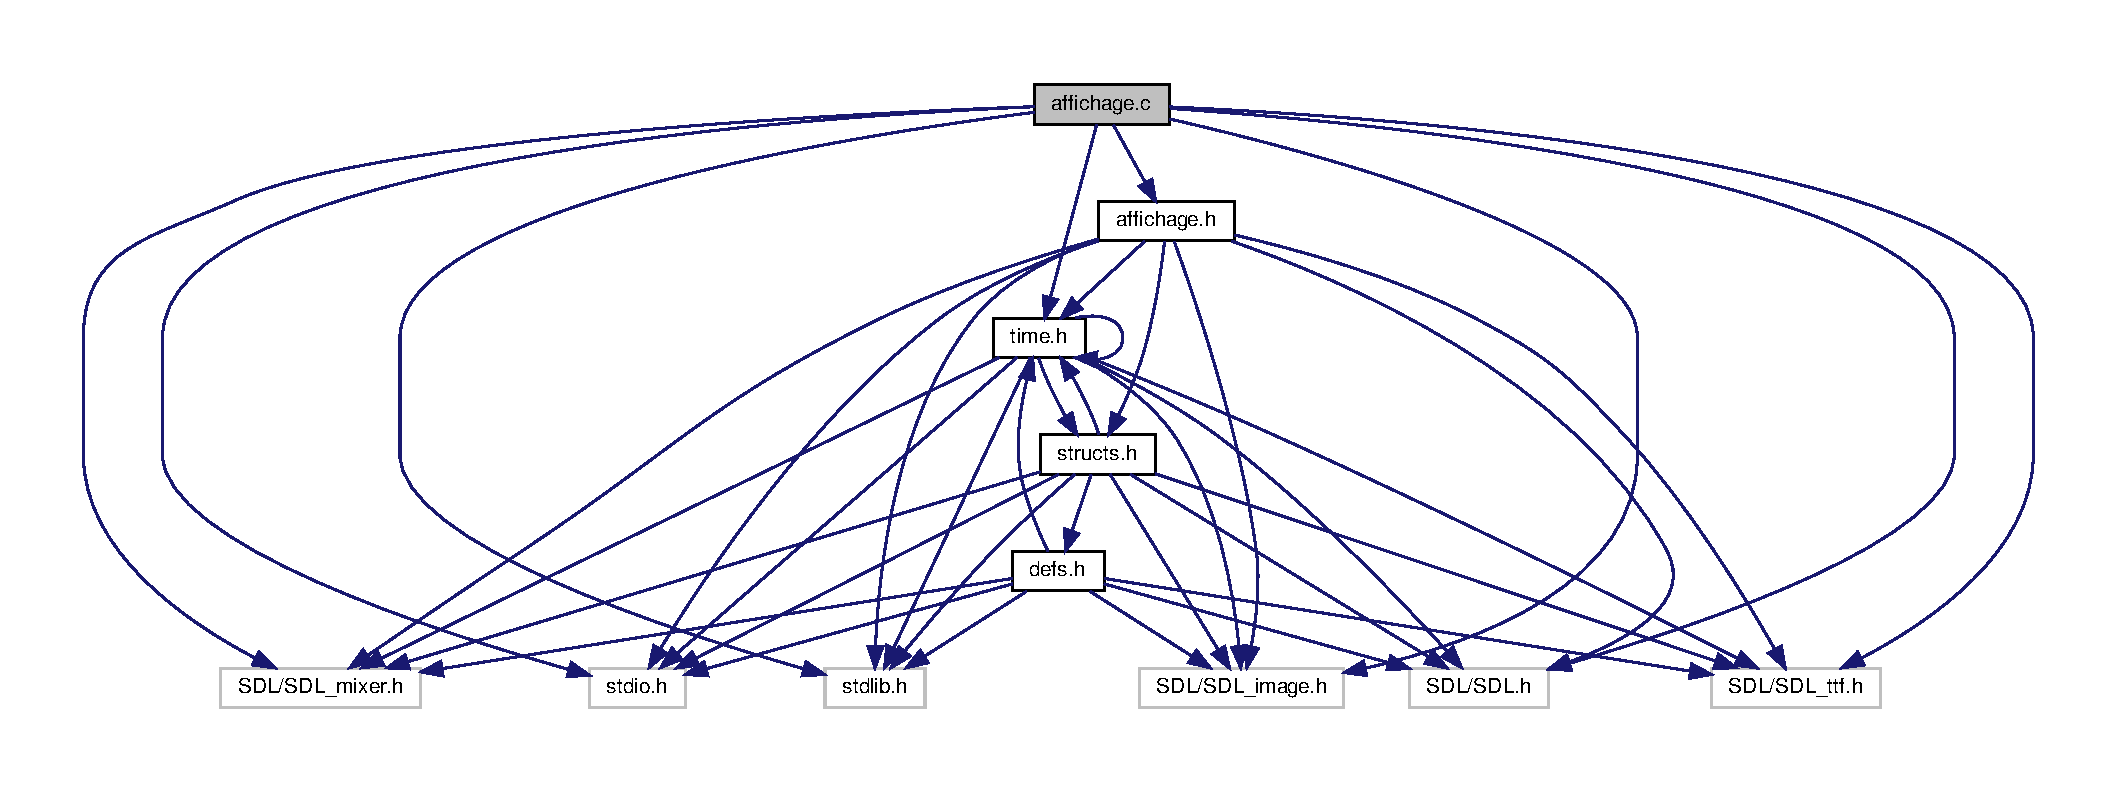
\includegraphics[width=350pt]{affichage_8c__incl}
\end{center}
\end{figure}
\subsection*{Functions}
\begin{DoxyCompactItemize}
\item 
\mbox{\Hypertarget{affichage_8c_a3f6c2eca93b030bcce2a888c2b37f9c8}\label{affichage_8c_a3f6c2eca93b030bcce2a888c2b37f9c8}} 
void {\bfseries afficher\+Image} (void)
\item 
\mbox{\Hypertarget{affichage_8c_a1b74701ddf3945435e0bb81ee57a3925}\label{affichage_8c_a1b74701ddf3945435e0bb81ee57a3925}} 
void {\bfseries draw\+Image} (S\+D\+L\+\_\+\+Surface $\ast$image, int x, int y)
\item 
\mbox{\Hypertarget{affichage_8c_a2b2add8c7e75f279cebe69b80c08629a}\label{affichage_8c_a2b2add8c7e75f279cebe69b80c08629a}} 
void {\bfseries afficher} (void)
\item 
\mbox{\Hypertarget{affichage_8c_a12b9f50e1f51a4019b2b5cb8c8ed04b8}\label{affichage_8c_a12b9f50e1f51a4019b2b5cb8c8ed04b8}} 
S\+D\+L\+\_\+\+Surface $\ast$ {\bfseries load\+Image} (char $\ast$name)
\item 
\mbox{\Hypertarget{affichage_8c_a278a2ffbb995f7837d4970a4d7435b63}\label{affichage_8c_a278a2ffbb995f7837d4970a4d7435b63}} 
void {\bfseries delay} (unsigned int frame\+Limit)
\item 
\mbox{\Hypertarget{affichage_8c_aa76da22e7509758d8e452d6fd6fb924a}\label{affichage_8c_aa76da22e7509758d8e452d6fd6fb924a}} 
void {\bfseries draw\+Hud} (void)
\end{DoxyCompactItemize}


\subsection{Detailed Description}
affichage libs 

\begin{DoxyAuthor}{Author}
Youssef 
\end{DoxyAuthor}
\begin{DoxyVersion}{Version}
1.\+0 
\end{DoxyVersion}
\begin{DoxyDate}{Date}
07/06/2020 
\end{DoxyDate}

\hypertarget{affichage_8h}{}\section{affichage.\+h File Reference}
\label{affichage_8h}\index{affichage.\+h@{affichage.\+h}}


affichage libs  


{\ttfamily \#include $<$stdlib.\+h$>$}\newline
{\ttfamily \#include $<$stdio.\+h$>$}\newline
{\ttfamily \#include $<$S\+D\+L/\+S\+D\+L.\+h$>$}\newline
{\ttfamily \#include $<$S\+D\+L/\+S\+D\+L\+\_\+image.\+h$>$}\newline
{\ttfamily \#include $<$S\+D\+L/\+S\+D\+L\+\_\+mixer.\+h$>$}\newline
{\ttfamily \#include $<$S\+D\+L/\+S\+D\+L\+\_\+ttf.\+h$>$}\newline
{\ttfamily \#include $<$time.\+h$>$}\newline
{\ttfamily \#include \char`\"{}structs.\+h\char`\"{}}\newline
Include dependency graph for affichage.\+h\+:
\nopagebreak
\begin{figure}[H]
\begin{center}
\leavevmode
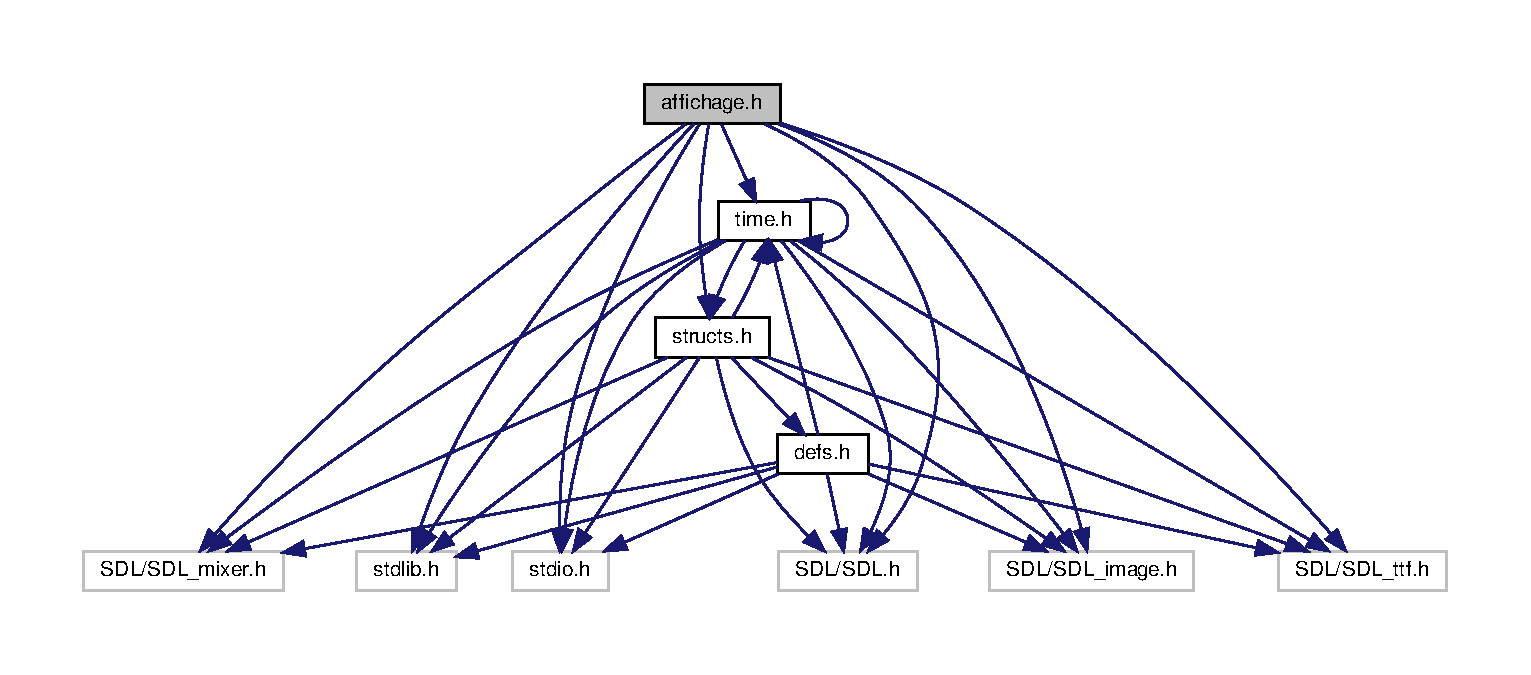
\includegraphics[width=350pt]{affichage_8h__incl}
\end{center}
\end{figure}
This graph shows which files directly or indirectly include this file\+:
\nopagebreak
\begin{figure}[H]
\begin{center}
\leavevmode
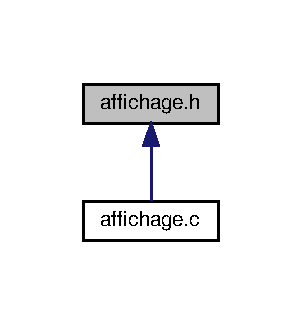
\includegraphics[width=145pt]{affichage_8h__dep__incl}
\end{center}
\end{figure}
\subsection*{Functions}
\begin{DoxyCompactItemize}
\item 
\mbox{\Hypertarget{affichage_8h_a6919db37a5bef552f77bfa3c5513d0dc}\label{affichage_8h_a6919db37a5bef552f77bfa3c5513d0dc}} 
void {\bfseries afficherplayer} (void)
\item 
\mbox{\Hypertarget{affichage_8h_a4af74196df835ca0c26544f742f559f7}\label{affichage_8h_a4af74196df835ca0c26544f742f559f7}} 
void {\bfseries afficher\+Monster} (void)
\item 
\mbox{\Hypertarget{affichage_8h_a892dff0e9ccf5c01d1a4a5a4958310a8}\label{affichage_8h_a892dff0e9ccf5c01d1a4a5a4958310a8}} 
void {\bfseries animationplayer} (void)
\item 
\mbox{\Hypertarget{affichage_8h_ada0ea8cc9045ddf00fad03ae738f10ea}\label{affichage_8h_ada0ea8cc9045ddf00fad03ae738f10ea}} 
void {\bfseries animation\+Monster} (void)
\item 
\mbox{\Hypertarget{affichage_8h_aa76da22e7509758d8e452d6fd6fb924a}\label{affichage_8h_aa76da22e7509758d8e452d6fd6fb924a}} 
void {\bfseries draw\+Hud} (void)
\item 
\mbox{\Hypertarget{affichage_8h_a2b2add8c7e75f279cebe69b80c08629a}\label{affichage_8h_a2b2add8c7e75f279cebe69b80c08629a}} 
void {\bfseries afficher} (void)
\item 
\mbox{\Hypertarget{affichage_8h_a83d0894aca32e4162ff85241c123286c}\label{affichage_8h_a83d0894aca32e4162ff85241c123286c}} 
void {\bfseries draw\+String} (char $\ast$text, int x, int y, T\+T\+F\+\_\+\+Font $\ast$font)
\item 
\mbox{\Hypertarget{affichage_8h_af646d273a1348946bb843f25e39a58bb}\label{affichage_8h_af646d273a1348946bb843f25e39a58bb}} 
void {\bfseries draw\+\_\+\+String} (char $\ast$text, int x, int y, T\+T\+F\+\_\+\+Font $\ast$font)
\item 
\mbox{\Hypertarget{affichage_8h_a3c3e683a005eace2dd1e4d551056d9b6}\label{affichage_8h_a3c3e683a005eace2dd1e4d551056d9b6}} 
void {\bfseries timer} ()
\item 
\mbox{\Hypertarget{affichage_8h_ac1dd451bf94ab9d190866bf42aad3dbd}\label{affichage_8h_ac1dd451bf94ab9d190866bf42aad3dbd}} 
void {\bfseries Afficher\+\_\+\+Minimap} (S\+D\+L\+\_\+\+Surface $\ast$screen, S\+D\+L\+\_\+\+Rect posplayer, S\+D\+L\+\_\+\+Rect posmonster, S\+D\+L\+\_\+\+Rect posstar)
\end{DoxyCompactItemize}
\subsection*{Variables}
\begin{DoxyCompactItemize}
\item 
\mbox{\Hypertarget{affichage_8h_abbeff4ee7b328d6b61b563ecded5bf83}\label{affichage_8h_abbeff4ee7b328d6b61b563ecded5bf83}} 
\hyperlink{structGestion}{Gestion} {\bfseries jeu}
\item 
\mbox{\Hypertarget{affichage_8h_ac9becb8e2f80125547c8cc8f9d56b7ab}\label{affichage_8h_ac9becb8e2f80125547c8cc8f9d56b7ab}} 
\hyperlink{structMap}{Map} {\bfseries map}
\item 
\mbox{\Hypertarget{affichage_8h_a32175bc9c482ed465d43f3e1d31f72a4}\label{affichage_8h_a32175bc9c482ed465d43f3e1d31f72a4}} 
\hyperlink{structGameobject}{Gameobject} {\bfseries star}
\item 
\mbox{\Hypertarget{affichage_8h_abf5bfa705e66ffc1ddaa6ce46c960873}\label{affichage_8h_abf5bfa705e66ffc1ddaa6ce46c960873}} 
T\+T\+F\+\_\+\+Font $\ast$ {\bfseries font}
\item 
\mbox{\Hypertarget{affichage_8h_a2737dcd286631af70eac9ebd6de78a07}\label{affichage_8h_a2737dcd286631af70eac9ebd6de78a07}} 
\hyperlink{structHero}{Hero} {\bfseries monster}
\item 
\mbox{\Hypertarget{affichage_8h_a7a56ddcc26459f1d1b0391d1a2025448}\label{affichage_8h_a7a56ddcc26459f1d1b0391d1a2025448}} 
\hyperlink{structHero}{Hero} {\bfseries player}
\end{DoxyCompactItemize}


\subsection{Detailed Description}
affichage libs 

\begin{DoxyAuthor}{Author}
Youssef 
\end{DoxyAuthor}
\begin{DoxyVersion}{Version}
1.\+0 
\end{DoxyVersion}
\begin{DoxyDate}{Date}
07/06/2020 
\end{DoxyDate}

\hypertarget{animation_8c}{}\section{animation.\+c File Reference}
\label{animation_8c}\index{animation.\+c@{animation.\+c}}


animation libs  


{\ttfamily \#include $<$stdlib.\+h$>$}\newline
{\ttfamily \#include $<$stdio.\+h$>$}\newline
{\ttfamily \#include $<$S\+D\+L/\+S\+D\+L.\+h$>$}\newline
{\ttfamily \#include $<$S\+D\+L/\+S\+D\+L\+\_\+image.\+h$>$}\newline
{\ttfamily \#include $<$S\+D\+L/\+S\+D\+L\+\_\+mixer.\+h$>$}\newline
{\ttfamily \#include $<$S\+D\+L/\+S\+D\+L\+\_\+ttf.\+h$>$}\newline
{\ttfamily \#include $<$time.\+h$>$}\newline
{\ttfamily \#include \char`\"{}animation.\+h\char`\"{}}\newline
Include dependency graph for animation.\+c\+:
\nopagebreak
\begin{figure}[H]
\begin{center}
\leavevmode
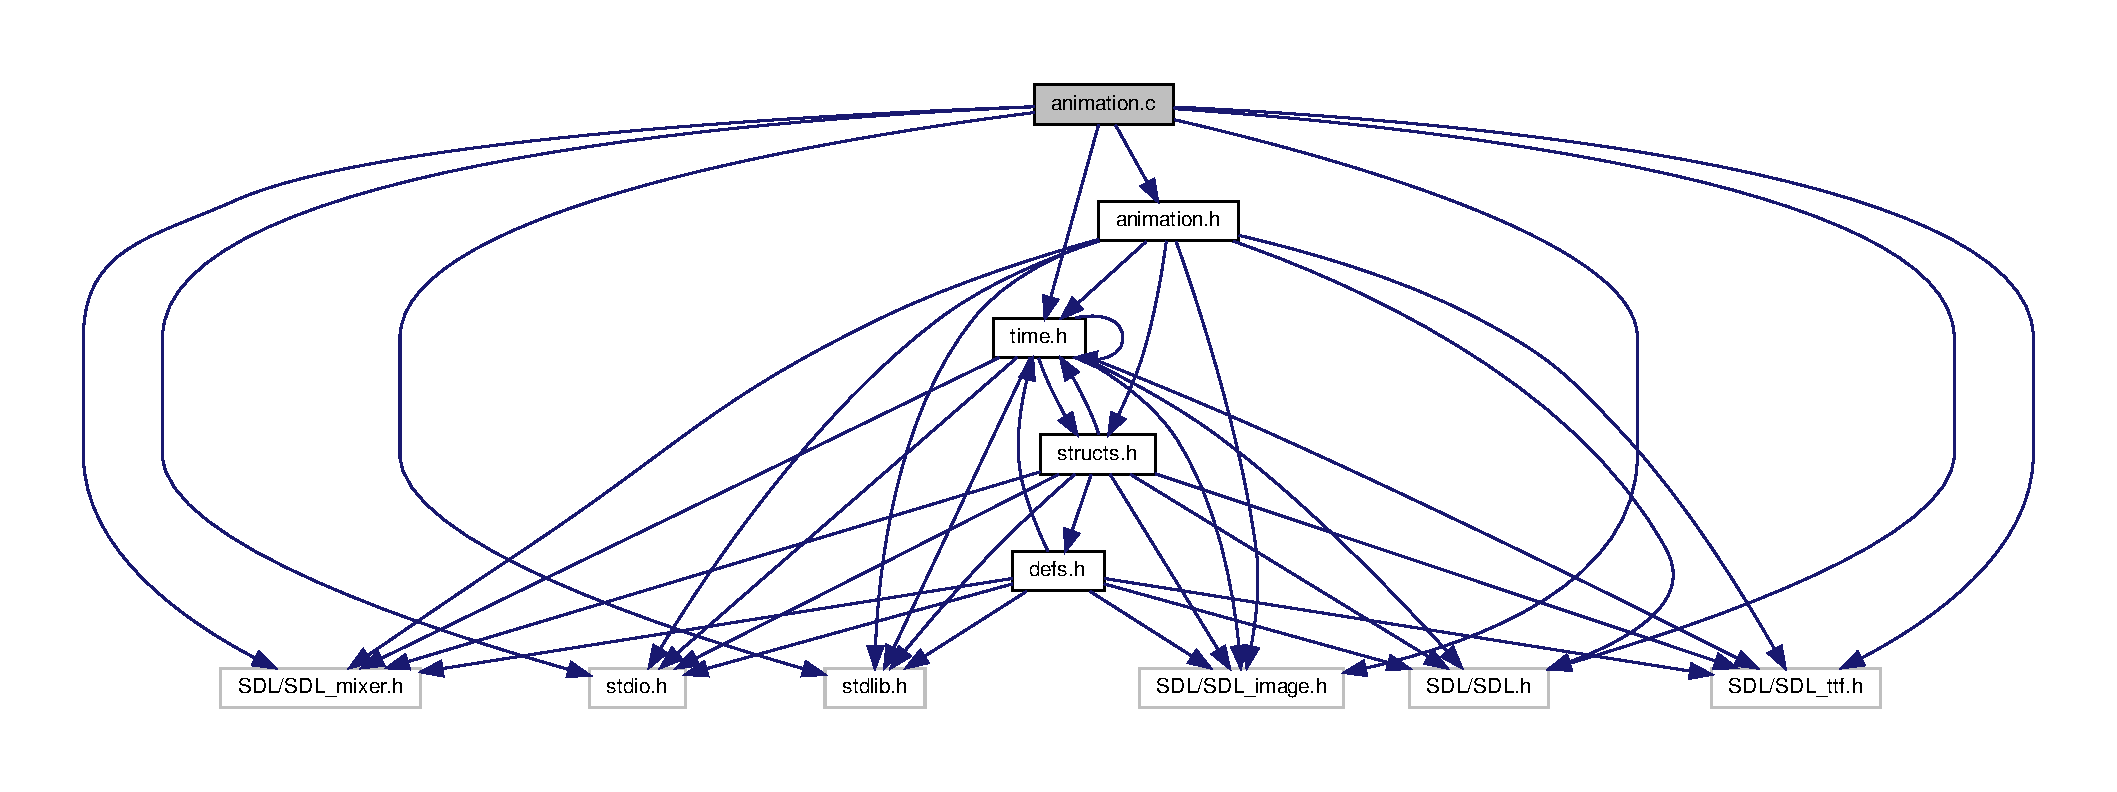
\includegraphics[width=350pt]{animation_8c__incl}
\end{center}
\end{figure}
\subsection*{Functions}
\begin{DoxyCompactItemize}
\item 
\mbox{\Hypertarget{animation_8c_ae535c192238ff0f42284c93a962411b1}\label{animation_8c_ae535c192238ff0f42284c93a962411b1}} 
void {\bfseries animationplayer} ()
\item 
\mbox{\Hypertarget{animation_8c_ada0ea8cc9045ddf00fad03ae738f10ea}\label{animation_8c_ada0ea8cc9045ddf00fad03ae738f10ea}} 
void {\bfseries animation\+Monster} (void)
\item 
\mbox{\Hypertarget{animation_8c_ae79e00c8c17b1a8ba7cf841be6cd0ffd}\label{animation_8c_ae79e00c8c17b1a8ba7cf841be6cd0ffd}} 
void {\bfseries change\+Animation} (\hyperlink{structHero}{Hero} $\ast$entity, char $\ast$name)
\end{DoxyCompactItemize}


\subsection{Detailed Description}
animation libs 

\begin{DoxyAuthor}{Author}
Raed+\+Yasmine+\+Youssef 
\end{DoxyAuthor}
\begin{DoxyVersion}{Version}
1.\+0 
\end{DoxyVersion}
\begin{DoxyDate}{Date}
07/06/2020 
\end{DoxyDate}

\hypertarget{animation_8h}{}\section{animation.\+h File Reference}
\label{animation_8h}\index{animation.\+h@{animation.\+h}}


animation libs  


{\ttfamily \#include $<$stdlib.\+h$>$}\newline
{\ttfamily \#include $<$stdio.\+h$>$}\newline
{\ttfamily \#include $<$S\+D\+L/\+S\+D\+L.\+h$>$}\newline
{\ttfamily \#include $<$S\+D\+L/\+S\+D\+L\+\_\+image.\+h$>$}\newline
{\ttfamily \#include $<$S\+D\+L/\+S\+D\+L\+\_\+mixer.\+h$>$}\newline
{\ttfamily \#include $<$S\+D\+L/\+S\+D\+L\+\_\+ttf.\+h$>$}\newline
{\ttfamily \#include $<$time.\+h$>$}\newline
{\ttfamily \#include \char`\"{}structs.\+h\char`\"{}}\newline
Include dependency graph for animation.\+h\+:
\nopagebreak
\begin{figure}[H]
\begin{center}
\leavevmode
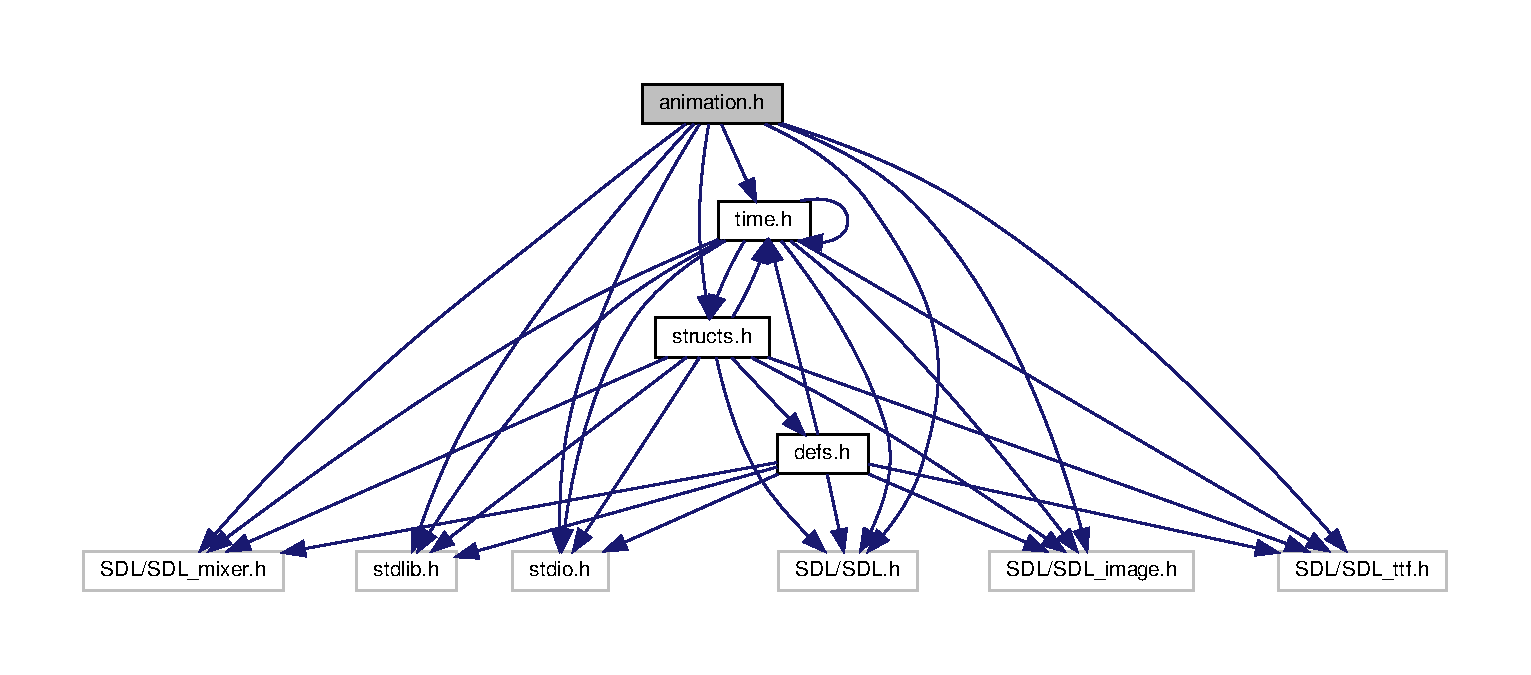
\includegraphics[width=350pt]{animation_8h__incl}
\end{center}
\end{figure}
This graph shows which files directly or indirectly include this file\+:
\nopagebreak
\begin{figure}[H]
\begin{center}
\leavevmode
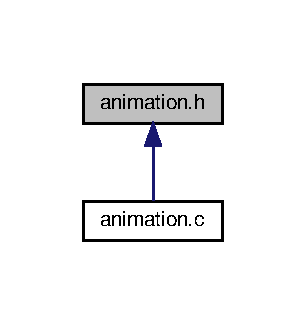
\includegraphics[width=147pt]{animation_8h__dep__incl}
\end{center}
\end{figure}
\subsection*{Functions}
\begin{DoxyCompactItemize}
\item 
\mbox{\Hypertarget{animation_8h_a12b9f50e1f51a4019b2b5cb8c8ed04b8}\label{animation_8h_a12b9f50e1f51a4019b2b5cb8c8ed04b8}} 
S\+D\+L\+\_\+\+Surface $\ast$ {\bfseries load\+Image} (char $\ast$name)
\item 
\mbox{\Hypertarget{animation_8h_a6919db37a5bef552f77bfa3c5513d0dc}\label{animation_8h_a6919db37a5bef552f77bfa3c5513d0dc}} 
void {\bfseries afficherplayer} (void)
\item 
\mbox{\Hypertarget{animation_8h_a4af74196df835ca0c26544f742f559f7}\label{animation_8h_a4af74196df835ca0c26544f742f559f7}} 
void {\bfseries afficher\+Monster} (void)
\end{DoxyCompactItemize}
\subsection*{Variables}
\begin{DoxyCompactItemize}
\item 
\mbox{\Hypertarget{animation_8h_abbeff4ee7b328d6b61b563ecded5bf83}\label{animation_8h_abbeff4ee7b328d6b61b563ecded5bf83}} 
\hyperlink{structGestion}{Gestion} {\bfseries jeu}
\item 
\mbox{\Hypertarget{animation_8h_a7a56ddcc26459f1d1b0391d1a2025448}\label{animation_8h_a7a56ddcc26459f1d1b0391d1a2025448}} 
\hyperlink{structHero}{Hero} {\bfseries player}
\item 
\mbox{\Hypertarget{animation_8h_a2737dcd286631af70eac9ebd6de78a07}\label{animation_8h_a2737dcd286631af70eac9ebd6de78a07}} 
\hyperlink{structHero}{Hero} {\bfseries monster}
\item 
\mbox{\Hypertarget{animation_8h_ad4db59ccea8946af2bb70f8269e99eeb}\label{animation_8h_ad4db59ccea8946af2bb70f8269e99eeb}} 
\hyperlink{structInput}{Input} {\bfseries input}
\end{DoxyCompactItemize}


\subsection{Detailed Description}
animation libs 

\begin{DoxyAuthor}{Author}
Raed+\+Yasmine+\+Youssef 
\end{DoxyAuthor}
\begin{DoxyVersion}{Version}
1.\+0 
\end{DoxyVersion}
\begin{DoxyDate}{Date}
07/06/2020 
\end{DoxyDate}

\hypertarget{arduino_8c}{}\section{arduino.\+c File Reference}
\label{arduino_8c}\index{arduino.\+c@{arduino.\+c}}


arduino libs  


{\ttfamily \#include $<$stdlib.\+h$>$}\newline
{\ttfamily \#include $<$stdio.\+h$>$}\newline
{\ttfamily \#include $<$S\+D\+L/\+S\+D\+L.\+h$>$}\newline
{\ttfamily \#include $<$S\+D\+L/\+S\+D\+L\+\_\+image.\+h$>$}\newline
{\ttfamily \#include $<$S\+D\+L/\+S\+D\+L\+\_\+mixer.\+h$>$}\newline
{\ttfamily \#include $<$S\+D\+L/\+S\+D\+L\+\_\+ttf.\+h$>$}\newline
{\ttfamily \#include $<$time.\+h$>$}\newline
{\ttfamily \#include \char`\"{}arduino.\+h\char`\"{}}\newline
Include dependency graph for arduino.\+c\+:
\nopagebreak
\begin{figure}[H]
\begin{center}
\leavevmode
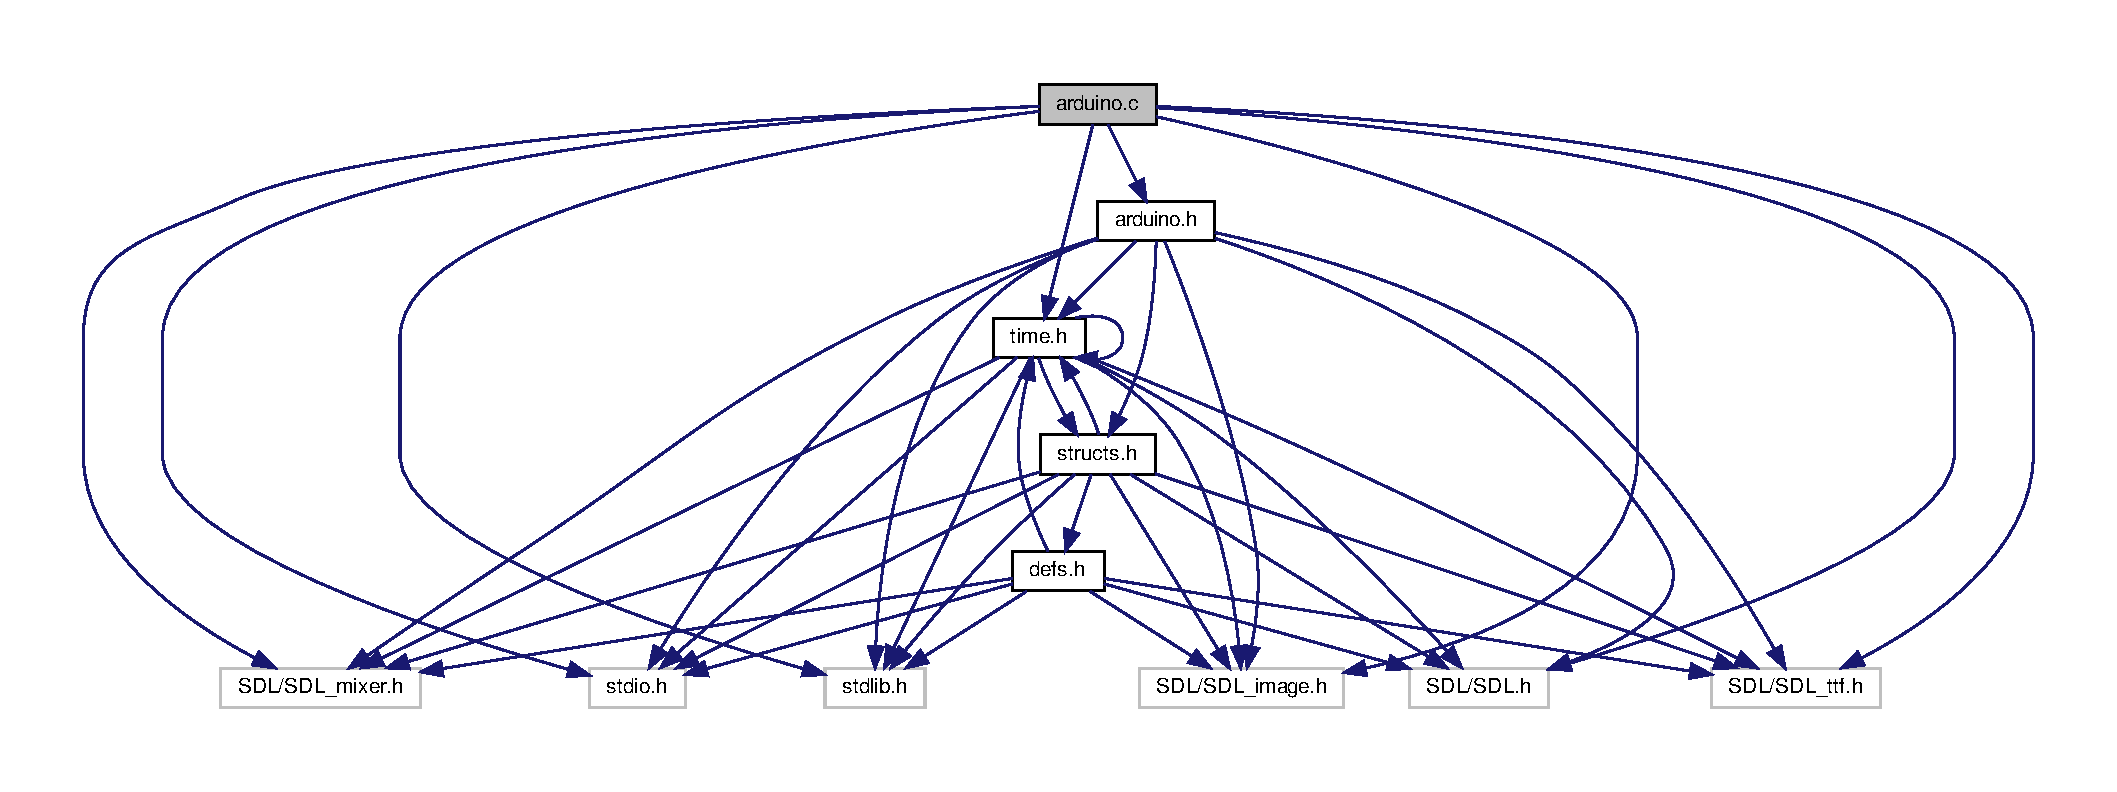
\includegraphics[width=350pt]{arduino_8c__incl}
\end{center}
\end{figure}
\subsection*{Functions}
\begin{DoxyCompactItemize}
\item 
\mbox{\Hypertarget{arduino_8c_ab8fc8c25e0629a19256ad4f266b65018}\label{arduino_8c_ab8fc8c25e0629a19256ad4f266b65018}} 
int {\bfseries arduino\+Write\+Data} (int x)
\item 
\mbox{\Hypertarget{arduino_8c_af26975b0e6c2018b62f8f188392ffba8}\label{arduino_8c_af26975b0e6c2018b62f8f188392ffba8}} 
int {\bfseries arduino\+Read\+Data} (int $\ast$x)
\end{DoxyCompactItemize}


\subsection{Detailed Description}
arduino libs 

\begin{DoxyAuthor}{Author}
Dynamic 
\end{DoxyAuthor}
\begin{DoxyVersion}{Version}
1.\+0 
\end{DoxyVersion}
\begin{DoxyDate}{Date}
07/06/2020 
\end{DoxyDate}

\hypertarget{arduino_8h}{}\section{arduino.\+h File Reference}
\label{arduino_8h}\index{arduino.\+h@{arduino.\+h}}


arduino libs  


{\ttfamily \#include $<$stdlib.\+h$>$}\newline
{\ttfamily \#include $<$stdio.\+h$>$}\newline
{\ttfamily \#include $<$S\+D\+L/\+S\+D\+L.\+h$>$}\newline
{\ttfamily \#include $<$S\+D\+L/\+S\+D\+L\+\_\+image.\+h$>$}\newline
{\ttfamily \#include $<$S\+D\+L/\+S\+D\+L\+\_\+mixer.\+h$>$}\newline
{\ttfamily \#include $<$S\+D\+L/\+S\+D\+L\+\_\+ttf.\+h$>$}\newline
{\ttfamily \#include $<$time.\+h$>$}\newline
{\ttfamily \#include \char`\"{}structs.\+h\char`\"{}}\newline
Include dependency graph for arduino.\+h\+:
\nopagebreak
\begin{figure}[H]
\begin{center}
\leavevmode
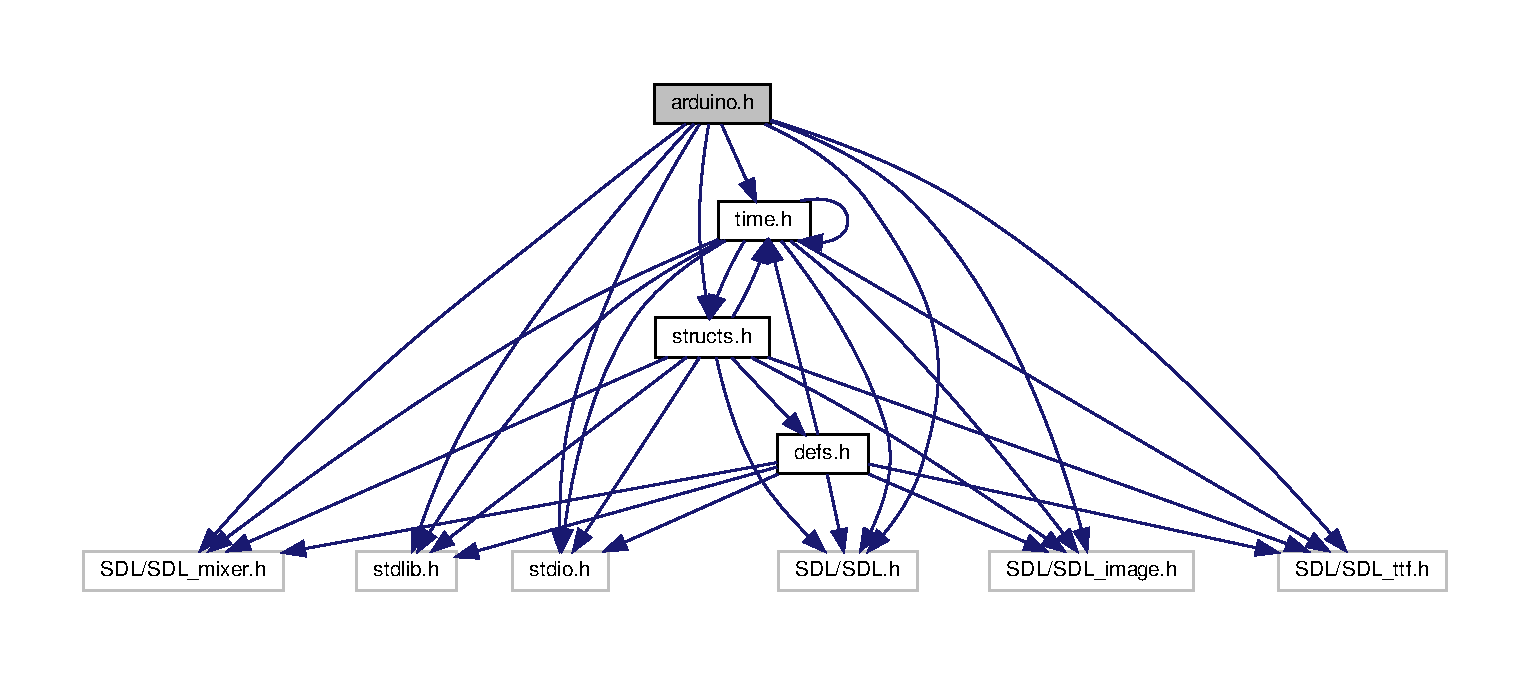
\includegraphics[width=350pt]{arduino_8h__incl}
\end{center}
\end{figure}
This graph shows which files directly or indirectly include this file\+:
\nopagebreak
\begin{figure}[H]
\begin{center}
\leavevmode
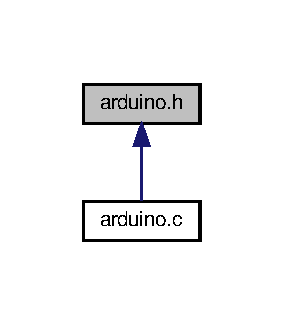
\includegraphics[width=136pt]{arduino_8h__dep__incl}
\end{center}
\end{figure}
\subsection*{Functions}
\begin{DoxyCompactItemize}
\item 
\mbox{\Hypertarget{arduino_8h_ab8fc8c25e0629a19256ad4f266b65018}\label{arduino_8h_ab8fc8c25e0629a19256ad4f266b65018}} 
int {\bfseries arduino\+Write\+Data} (int x)
\item 
\mbox{\Hypertarget{arduino_8h_af26975b0e6c2018b62f8f188392ffba8}\label{arduino_8h_af26975b0e6c2018b62f8f188392ffba8}} 
int {\bfseries arduino\+Read\+Data} (int $\ast$x)
\end{DoxyCompactItemize}


\subsection{Detailed Description}
arduino libs 

\begin{DoxyAuthor}{Author}
Dynamic 
\end{DoxyAuthor}
\begin{DoxyVersion}{Version}
1.\+0 
\end{DoxyVersion}
\begin{DoxyDate}{Date}
07/06/2020 
\end{DoxyDate}

\hypertarget{collision_8c}{}\section{collision.\+c File Reference}
\label{collision_8c}\index{collision.\+c@{collision.\+c}}


collision libs  


{\ttfamily \#include $<$stdlib.\+h$>$}\newline
{\ttfamily \#include $<$stdio.\+h$>$}\newline
{\ttfamily \#include $<$S\+D\+L/\+S\+D\+L.\+h$>$}\newline
{\ttfamily \#include $<$S\+D\+L/\+S\+D\+L\+\_\+image.\+h$>$}\newline
{\ttfamily \#include $<$S\+D\+L/\+S\+D\+L\+\_\+mixer.\+h$>$}\newline
{\ttfamily \#include $<$S\+D\+L/\+S\+D\+L\+\_\+ttf.\+h$>$}\newline
{\ttfamily \#include $<$time.\+h$>$}\newline
{\ttfamily \#include \char`\"{}collision.\+h\char`\"{}}\newline
Include dependency graph for collision.\+c\+:
\nopagebreak
\begin{figure}[H]
\begin{center}
\leavevmode
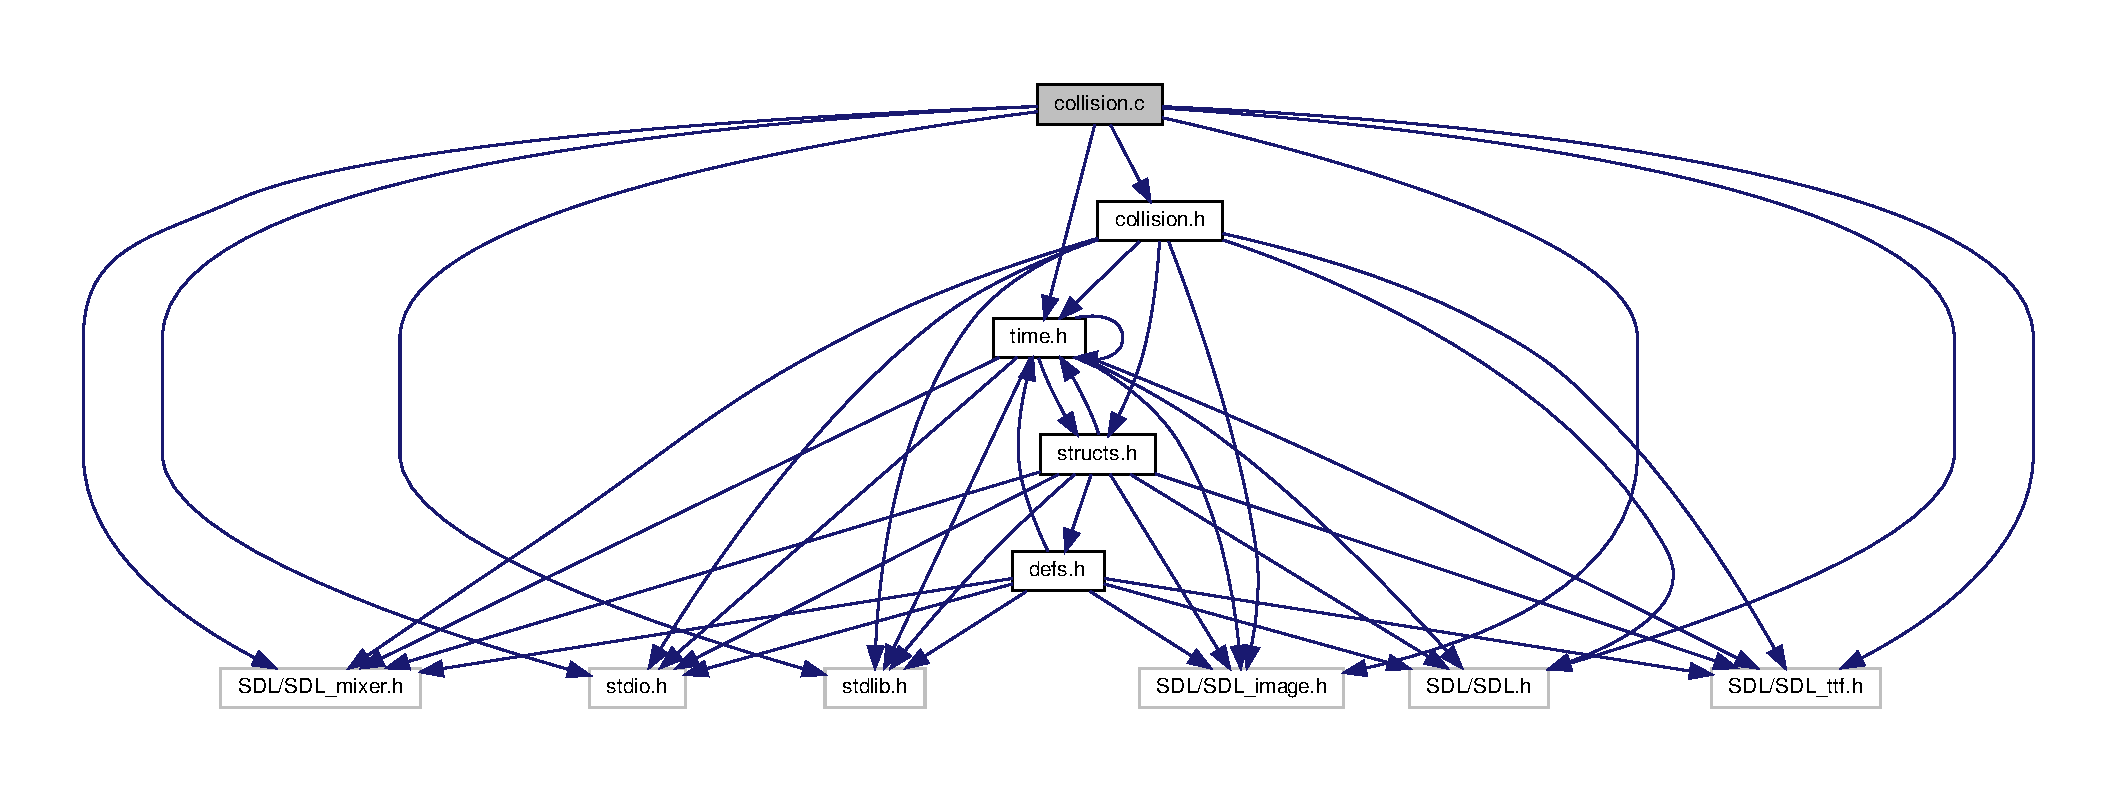
\includegraphics[width=350pt]{collision_8c__incl}
\end{center}
\end{figure}
\subsection*{Functions}
\begin{DoxyCompactItemize}
\item 
\mbox{\Hypertarget{collision_8c_a60470232937e2880d3669de86f905fd5}\label{collision_8c_a60470232937e2880d3669de86f905fd5}} 
int {\bfseries collision} ()
\end{DoxyCompactItemize}


\subsection{Detailed Description}
collision libs 

\begin{DoxyAuthor}{Author}
skander 
\end{DoxyAuthor}
\begin{DoxyVersion}{Version}
1.\+0 
\end{DoxyVersion}
\begin{DoxyDate}{Date}
07/06/2020 
\end{DoxyDate}

\hypertarget{collision_8h}{}\section{collision.\+h File Reference}
\label{collision_8h}\index{collision.\+h@{collision.\+h}}


collision libs  


{\ttfamily \#include $<$stdlib.\+h$>$}\newline
{\ttfamily \#include $<$stdio.\+h$>$}\newline
{\ttfamily \#include $<$S\+D\+L/\+S\+D\+L.\+h$>$}\newline
{\ttfamily \#include $<$S\+D\+L/\+S\+D\+L\+\_\+image.\+h$>$}\newline
{\ttfamily \#include $<$S\+D\+L/\+S\+D\+L\+\_\+mixer.\+h$>$}\newline
{\ttfamily \#include $<$S\+D\+L/\+S\+D\+L\+\_\+ttf.\+h$>$}\newline
{\ttfamily \#include $<$time.\+h$>$}\newline
{\ttfamily \#include \char`\"{}structs.\+h\char`\"{}}\newline
Include dependency graph for collision.\+h\+:
\nopagebreak
\begin{figure}[H]
\begin{center}
\leavevmode
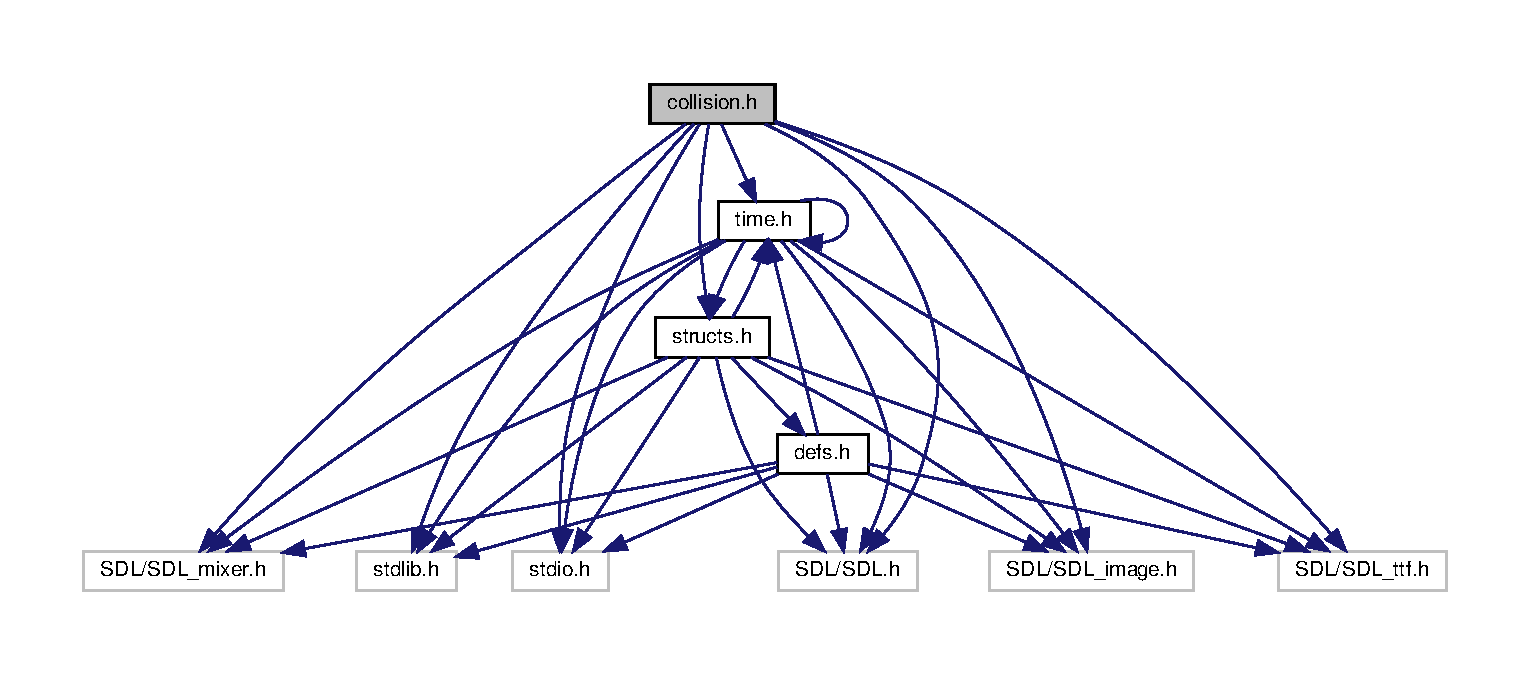
\includegraphics[width=350pt]{collision_8h__incl}
\end{center}
\end{figure}
This graph shows which files directly or indirectly include this file\+:
\nopagebreak
\begin{figure}[H]
\begin{center}
\leavevmode
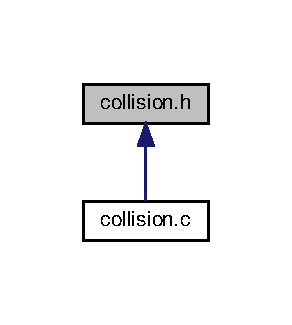
\includegraphics[width=140pt]{collision_8h__dep__incl}
\end{center}
\end{figure}
\subsection*{Functions}
\begin{DoxyCompactItemize}
\item 
\mbox{\Hypertarget{collision_8h_a60470232937e2880d3669de86f905fd5}\label{collision_8h_a60470232937e2880d3669de86f905fd5}} 
int {\bfseries collision} ()
\item 
\mbox{\Hypertarget{collision_8h_af6b3bf14e76f3d6bbda542457e8066a3}\label{collision_8h_af6b3bf14e76f3d6bbda542457e8066a3}} 
void {\bfseries Sound} (int type)
\end{DoxyCompactItemize}
\subsection*{Variables}
\begin{DoxyCompactItemize}
\item 
\mbox{\Hypertarget{collision_8h_a7a56ddcc26459f1d1b0391d1a2025448}\label{collision_8h_a7a56ddcc26459f1d1b0391d1a2025448}} 
\hyperlink{structHero}{Hero} {\bfseries player}
\item 
\mbox{\Hypertarget{collision_8h_a2737dcd286631af70eac9ebd6de78a07}\label{collision_8h_a2737dcd286631af70eac9ebd6de78a07}} 
\hyperlink{structHero}{Hero} {\bfseries monster}
\item 
\mbox{\Hypertarget{collision_8h_a46bbb8f0ca78423455fee2bbf4549165}\label{collision_8h_a46bbb8f0ca78423455fee2bbf4549165}} 
\hyperlink{structGameobject}{Gameobject} {\bfseries objet}
\item 
\mbox{\Hypertarget{collision_8h_a32175bc9c482ed465d43f3e1d31f72a4}\label{collision_8h_a32175bc9c482ed465d43f3e1d31f72a4}} 
\hyperlink{structGameobject}{Gameobject} {\bfseries star}
\item 
\mbox{\Hypertarget{collision_8h_abbeff4ee7b328d6b61b563ecded5bf83}\label{collision_8h_abbeff4ee7b328d6b61b563ecded5bf83}} 
\hyperlink{structGestion}{Gestion} {\bfseries jeu}
\end{DoxyCompactItemize}


\subsection{Detailed Description}
collision libs 

\begin{DoxyAuthor}{Author}
skander 
\end{DoxyAuthor}
\begin{DoxyVersion}{Version}
1.\+0 
\end{DoxyVersion}
\begin{DoxyDate}{Date}
07/06/2020 
\end{DoxyDate}

\hypertarget{defs_8h}{}\section{defs.\+h File Reference}
\label{defs_8h}\index{defs.\+h@{defs.\+h}}


defs libs  


{\ttfamily \#include $<$stdlib.\+h$>$}\newline
{\ttfamily \#include $<$stdio.\+h$>$}\newline
{\ttfamily \#include $<$S\+D\+L/\+S\+D\+L.\+h$>$}\newline
{\ttfamily \#include $<$S\+D\+L/\+S\+D\+L\+\_\+image.\+h$>$}\newline
{\ttfamily \#include $<$S\+D\+L/\+S\+D\+L\+\_\+mixer.\+h$>$}\newline
{\ttfamily \#include $<$S\+D\+L/\+S\+D\+L\+\_\+ttf.\+h$>$}\newline
{\ttfamily \#include $<$time.\+h$>$}\newline
Include dependency graph for defs.\+h\+:
\nopagebreak
\begin{figure}[H]
\begin{center}
\leavevmode
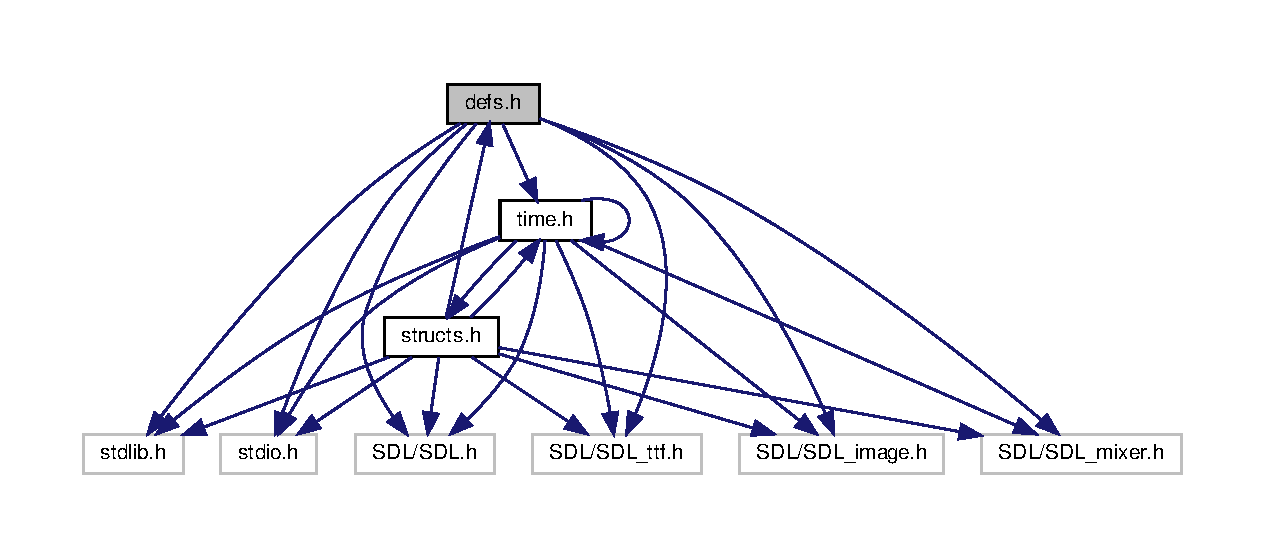
\includegraphics[width=350pt]{defs_8h__incl}
\end{center}
\end{figure}
This graph shows which files directly or indirectly include this file\+:
\nopagebreak
\begin{figure}[H]
\begin{center}
\leavevmode
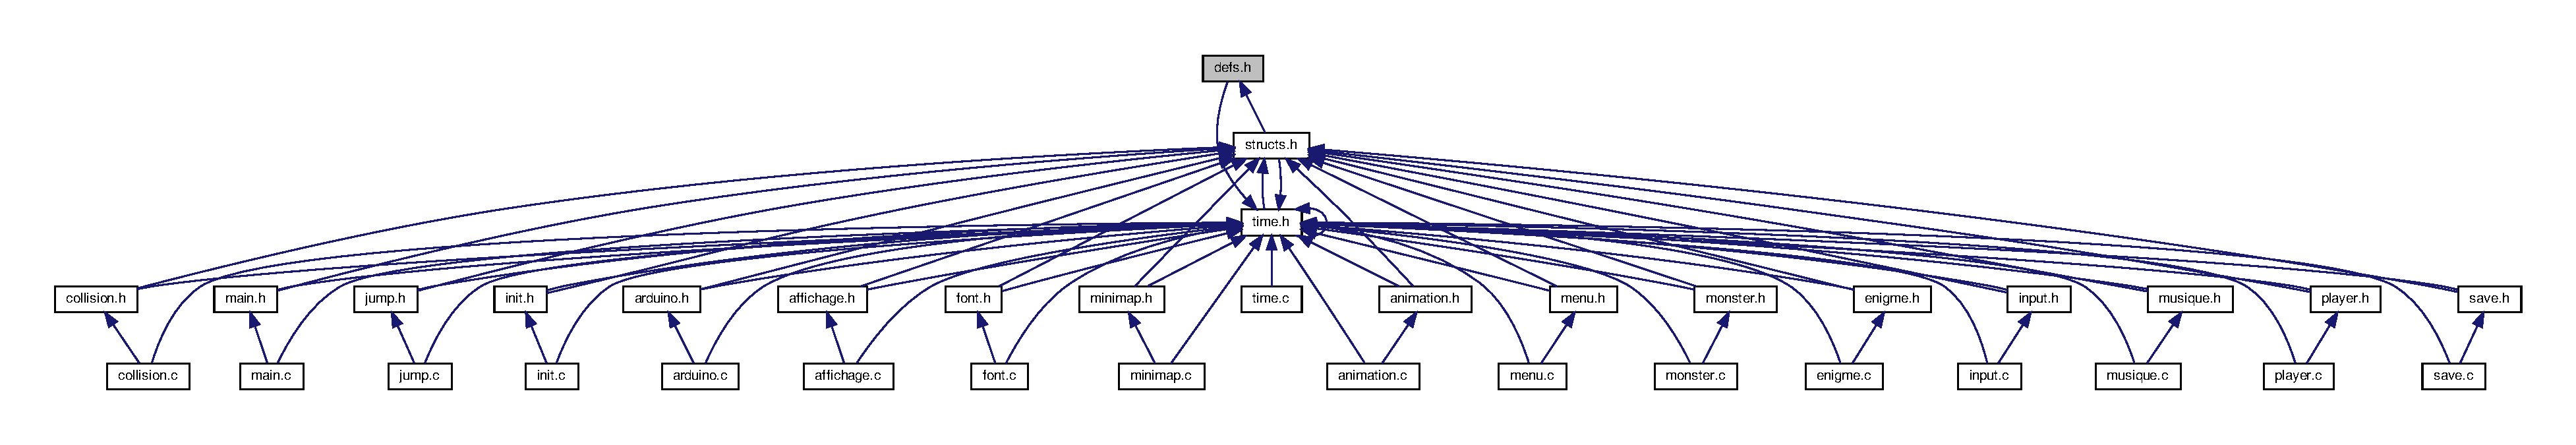
\includegraphics[width=350pt]{defs_8h__dep__incl}
\end{center}
\end{figure}
\subsection*{Macros}
\begin{DoxyCompactItemize}
\item 
\mbox{\Hypertarget{defs_8h_a2cd109632a6dcccaa80b43561b1ab700}\label{defs_8h_a2cd109632a6dcccaa80b43561b1ab700}} 
\#define {\bfseries S\+C\+R\+E\+E\+N\+\_\+\+W\+I\+D\+TH}~1200
\item 
\mbox{\Hypertarget{defs_8h_a6974d08a74da681b3957b2fead2608b8}\label{defs_8h_a6974d08a74da681b3957b2fead2608b8}} 
\#define {\bfseries S\+C\+R\+E\+E\+N\+\_\+\+H\+E\+I\+G\+HT}~480
\item 
\mbox{\Hypertarget{defs_8h_a5f5b551fce6993579430d7edd352e766}\label{defs_8h_a5f5b551fce6993579430d7edd352e766}} 
\#define {\bfseries T\+R\+A\+N\+S\+\_\+R}~255
\item 
\mbox{\Hypertarget{defs_8h_a2e05163a99bed3a22e4b6a0ab2ded999}\label{defs_8h_a2e05163a99bed3a22e4b6a0ab2ded999}} 
\#define {\bfseries T\+R\+A\+N\+S\+\_\+G}~0
\item 
\mbox{\Hypertarget{defs_8h_a5cca986885934b3dc2e524e63c379bcb}\label{defs_8h_a5cca986885934b3dc2e524e63c379bcb}} 
\#define {\bfseries T\+R\+A\+N\+S\+\_\+B}~255
\item 
\mbox{\Hypertarget{defs_8h_a55cc1ac28ac5a0acb73198f9259158be}\label{defs_8h_a55cc1ac28ac5a0acb73198f9259158be}} 
\#define {\bfseries P\+L\+A\+Y\+E\+R\+\_\+\+H\+E\+I\+G\+TH}~120
\item 
\mbox{\Hypertarget{defs_8h_a89e2ac9092225702ac543695d0771d38}\label{defs_8h_a89e2ac9092225702ac543695d0771d38}} 
\#define {\bfseries P\+L\+A\+Y\+E\+R\+\_\+\+W\+I\+D\+TH}~60
\item 
\mbox{\Hypertarget{defs_8h_a8e7bab1b185c829742f91a79142a7864}\label{defs_8h_a8e7bab1b185c829742f91a79142a7864}} 
\#define {\bfseries M\+O\+N\+S\+T\+E\+R\+\_\+\+W\+I\+D\+TH}~70
\item 
\mbox{\Hypertarget{defs_8h_a0f54805847ffae00e6f734ddd8e4c390}\label{defs_8h_a0f54805847ffae00e6f734ddd8e4c390}} 
\#define {\bfseries M\+O\+N\+S\+T\+E\+R\+\_\+\+H\+E\+I\+G\+TH}~74
\item 
\mbox{\Hypertarget{defs_8h_a0c464462edcc2e38d8f40be44005426b}\label{defs_8h_a0c464462edcc2e38d8f40be44005426b}} 
\#define {\bfseries T\+I\+M\+E\+\_\+\+B\+E\+T\+W\+E\+E\+N\+\_\+2\+\_\+\+F\+R\+A\+M\+ES}~8
\item 
\mbox{\Hypertarget{defs_8h_af49bad41acef45feb40939c0cf9d5d35}\label{defs_8h_af49bad41acef45feb40939c0cf9d5d35}} 
\#define {\bfseries P\+L\+A\+Y\+E\+R\+\_\+\+S\+P\+E\+ED}~4
\item 
\mbox{\Hypertarget{defs_8h_a27b5922e9871cc546a163c698edda2d5}\label{defs_8h_a27b5922e9871cc546a163c698edda2d5}} 
\#define {\bfseries P\+L\+A\+Y\+E\+R\+\_\+\+J\+U\+MP}~2.\+7
\item 
\mbox{\Hypertarget{defs_8h_af627f18bf33b5a06da62e5f2475c806a}\label{defs_8h_af627f18bf33b5a06da62e5f2475c806a}} 
\#define {\bfseries O\+N\+\_\+\+G\+R\+O\+U\+ND}~264
\item 
\mbox{\Hypertarget{defs_8h_a4083fcbe80d42575b0336ddbf4ebc622}\label{defs_8h_a4083fcbe80d42575b0336ddbf4ebc622}} 
\#define {\bfseries W\+A\+LK}~1
\item 
\mbox{\Hypertarget{defs_8h_aee551d17fffb6235cc7123499dbf7d65}\label{defs_8h_aee551d17fffb6235cc7123499dbf7d65}} 
\#define {\bfseries J\+U\+MP}~2
\item 
\mbox{\Hypertarget{defs_8h_a80fb826a684cf3f0d306b22aa100ddac}\label{defs_8h_a80fb826a684cf3f0d306b22aa100ddac}} 
\#define {\bfseries R\+I\+G\+HT}~1
\item 
\mbox{\Hypertarget{defs_8h_a437ef08681e7210d6678427030446a54}\label{defs_8h_a437ef08681e7210d6678427030446a54}} 
\#define {\bfseries L\+E\+FT}~2
\item 
\mbox{\Hypertarget{defs_8h_a57f4734a69c97a2adb1b42f20e26f846}\label{defs_8h_a57f4734a69c97a2adb1b42f20e26f846}} 
\#define {\bfseries D\+E\+A\+D\+\_\+\+Z\+O\+NE}~8000
\item 
\mbox{\Hypertarget{defs_8h_a1a13113f156dfb914f5e8330391c44ce}\label{defs_8h_a1a13113f156dfb914f5e8330391c44ce}} 
\#define {\bfseries B\+O\+U\+T\+O\+N\+\_\+\+H\+A\+UT}~2
\item 
\mbox{\Hypertarget{defs_8h_a23fee94314f1a72d113576daa9728fd3}\label{defs_8h_a23fee94314f1a72d113576daa9728fd3}} 
\#define {\bfseries B\+O\+U\+T\+O\+N\+\_\+\+B\+AS}~3
\item 
\mbox{\Hypertarget{defs_8h_a2c8798bbae83518169d7aaed452c05ed}\label{defs_8h_a2c8798bbae83518169d7aaed452c05ed}} 
\#define {\bfseries B\+O\+U\+T\+O\+N\+\_\+\+G\+A\+U\+C\+HE}~4
\item 
\mbox{\Hypertarget{defs_8h_a38dbfb4101843fd2d618e6f92751014d}\label{defs_8h_a38dbfb4101843fd2d618e6f92751014d}} 
\#define {\bfseries B\+O\+U\+T\+O\+N\+\_\+\+D\+R\+O\+I\+TE}~5
\item 
\mbox{\Hypertarget{defs_8h_aedc455f9a6df35d47e126020119fd1ad}\label{defs_8h_aedc455f9a6df35d47e126020119fd1ad}} 
\#define {\bfseries B\+O\+U\+T\+O\+N\+\_\+\+S\+A\+UT}~7
\item 
\mbox{\Hypertarget{defs_8h_a20b242533b730dd3e97e51acec886521}\label{defs_8h_a20b242533b730dd3e97e51acec886521}} 
\#define {\bfseries B\+O\+U\+T\+O\+N\+\_\+\+P\+A\+U\+SE}~6
\end{DoxyCompactItemize}
\subsection*{Enumerations}
\begin{DoxyCompactItemize}
\item 
\mbox{\Hypertarget{defs_8h_a06fc87d81c62e9abb8790b6e5713c55b}\label{defs_8h_a06fc87d81c62e9abb8790b6e5713c55b}} 
enum \{ {\bfseries D\+E\+S\+T\+R\+OY}, 
{\bfseries S\+T\+AR}, 
{\bfseries B\+U\+T\+T\+ON}
 \}
\item 
\mbox{\Hypertarget{defs_8h_adf764cbdea00d65edcd07bb9953ad2b7}\label{defs_8h_adf764cbdea00d65edcd07bb9953ad2b7}} 
enum \{ {\bfseries S\+T\+A\+RT}, 
{\bfseries P\+A\+U\+SE}
 \}
\end{DoxyCompactItemize}


\subsection{Detailed Description}
defs libs 

\begin{DoxyAuthor}{Author}
Youssef 
\end{DoxyAuthor}
\begin{DoxyVersion}{Version}
1.\+0 
\end{DoxyVersion}
\begin{DoxyDate}{Date}
07/06/2020 
\end{DoxyDate}

\hypertarget{enigme_8c}{}\section{enigme.\+c File Reference}
\label{enigme_8c}\index{enigme.\+c@{enigme.\+c}}


enigme libs  


{\ttfamily \#include $<$stdlib.\+h$>$}\newline
{\ttfamily \#include $<$stdio.\+h$>$}\newline
{\ttfamily \#include $<$S\+D\+L/\+S\+D\+L.\+h$>$}\newline
{\ttfamily \#include $<$S\+D\+L/\+S\+D\+L\+\_\+image.\+h$>$}\newline
{\ttfamily \#include $<$S\+D\+L/\+S\+D\+L\+\_\+mixer.\+h$>$}\newline
{\ttfamily \#include $<$S\+D\+L/\+S\+D\+L\+\_\+ttf.\+h$>$}\newline
{\ttfamily \#include $<$time.\+h$>$}\newline
{\ttfamily \#include \char`\"{}enigme.\+h\char`\"{}}\newline
Include dependency graph for enigme.\+c\+:
\nopagebreak
\begin{figure}[H]
\begin{center}
\leavevmode
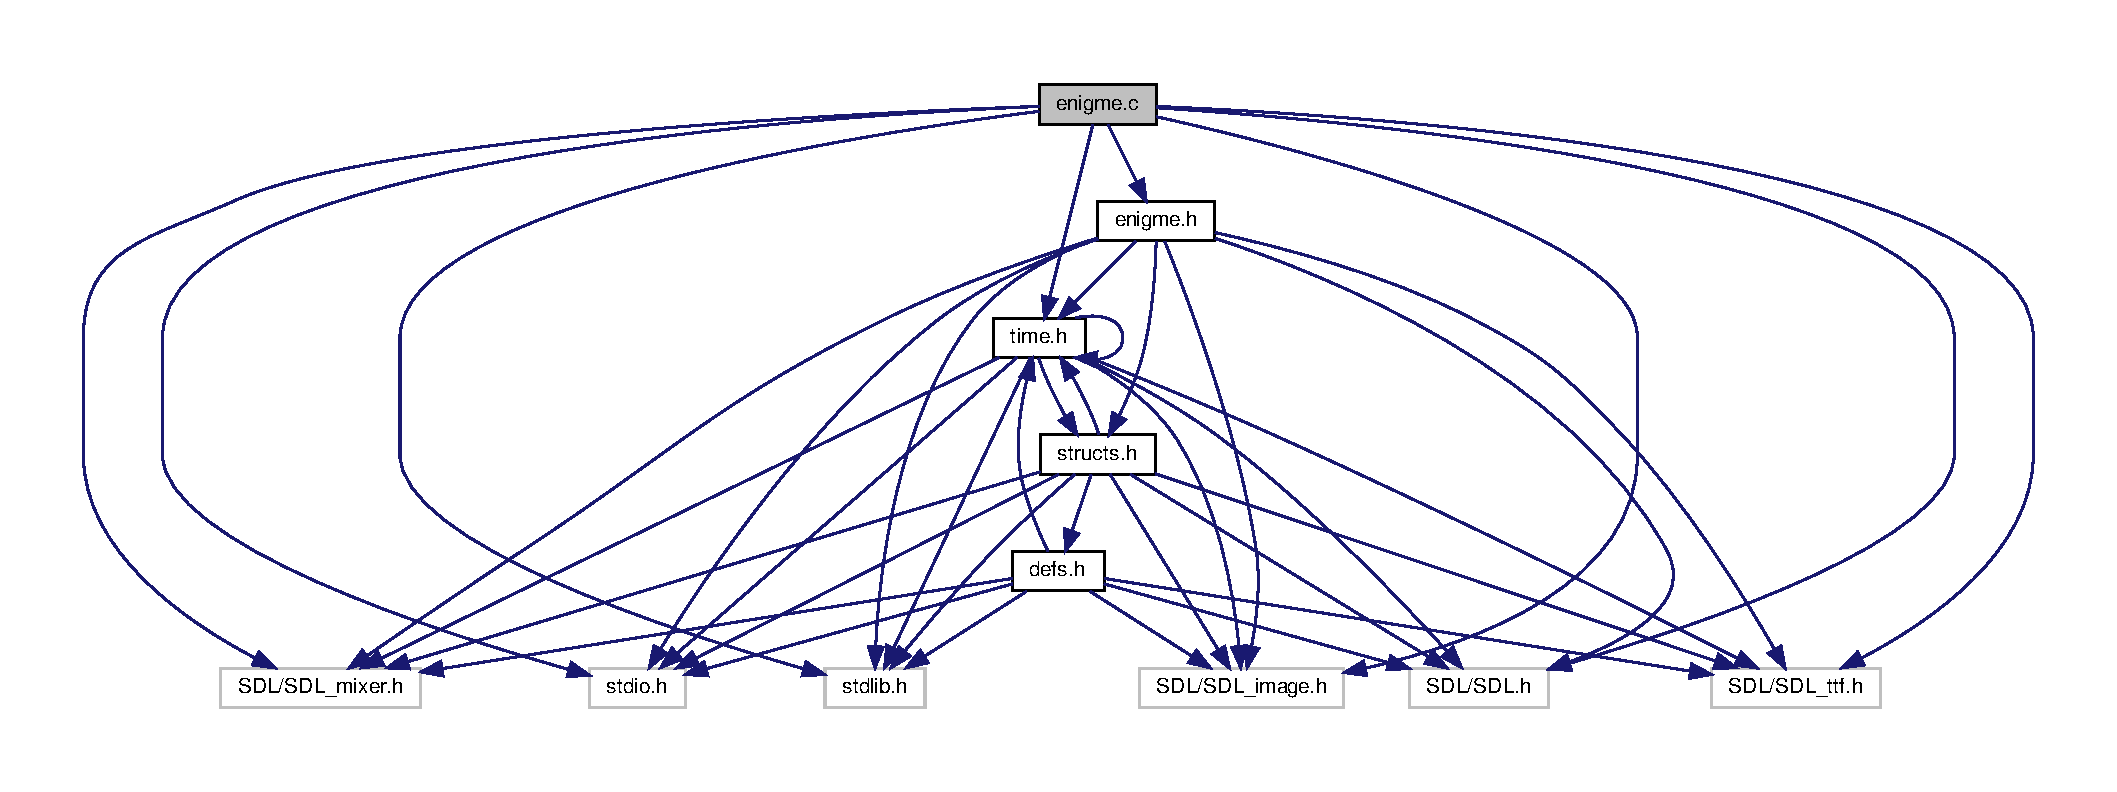
\includegraphics[width=350pt]{enigme_8c__incl}
\end{center}
\end{figure}
\subsection*{Functions}
\begin{DoxyCompactItemize}
\item 
\mbox{\Hypertarget{enigme_8c_a194546ea4fa1a0eaa63aacbac96f33bb}\label{enigme_8c_a194546ea4fa1a0eaa63aacbac96f33bb}} 
void {\bfseries init\+\_\+enigme} (\hyperlink{structenigme}{enigme} $\ast$e)
\item 
\mbox{\Hypertarget{enigme_8c_a345b17b765ec6a985fb162957d6e900c}\label{enigme_8c_a345b17b765ec6a985fb162957d6e900c}} 
void {\bfseries generate\+\_\+afficher} (S\+D\+L\+\_\+\+Surface $\ast$screen, char image \mbox{[}$\,$\mbox{]}, \hyperlink{structenigme}{enigme} $\ast$e, int $\ast$alea)
\item 
\mbox{\Hypertarget{enigme_8c_a6754b2ea5ab28613588b0286e5b0ce4c}\label{enigme_8c_a6754b2ea5ab28613588b0286e5b0ce4c}} 
int {\bfseries solution} (char image \mbox{[}$\,$\mbox{]})
\item 
\mbox{\Hypertarget{enigme_8c_ae855a03b9d7f7619bac3843306965df9}\label{enigme_8c_ae855a03b9d7f7619bac3843306965df9}} 
int {\bfseries resolution} (int $\ast$running, int $\ast$run)
\item 
\mbox{\Hypertarget{enigme_8c_a4000acf4af9607e9d50a33b70643a99a}\label{enigme_8c_a4000acf4af9607e9d50a33b70643a99a}} 
void {\bfseries afficher\+\_\+resultat} (S\+D\+L\+\_\+\+Surface $\ast$screen, int s, int r, \hyperlink{structenigme}{enigme} $\ast$en)
\item 
\mbox{\Hypertarget{enigme_8c_aa9512b1a048248682d54ec6f4c38e505}\label{enigme_8c_aa9512b1a048248682d54ec6f4c38e505}} 
void {\bfseries afficherenigme} ()
\end{DoxyCompactItemize}


\subsection{Detailed Description}
enigme libs 

\begin{DoxyAuthor}{Author}
Raed+\+Youssef 
\end{DoxyAuthor}
\begin{DoxyVersion}{Version}
1.\+0 
\end{DoxyVersion}
\begin{DoxyDate}{Date}
07/06/2020 
\end{DoxyDate}

\hypertarget{enigme_8h}{}\section{enigme.\+h File Reference}
\label{enigme_8h}\index{enigme.\+h@{enigme.\+h}}


enigme libs  


{\ttfamily \#include $<$stdlib.\+h$>$}\newline
{\ttfamily \#include $<$stdio.\+h$>$}\newline
{\ttfamily \#include $<$S\+D\+L/\+S\+D\+L.\+h$>$}\newline
{\ttfamily \#include $<$S\+D\+L/\+S\+D\+L\+\_\+image.\+h$>$}\newline
{\ttfamily \#include $<$S\+D\+L/\+S\+D\+L\+\_\+mixer.\+h$>$}\newline
{\ttfamily \#include $<$S\+D\+L/\+S\+D\+L\+\_\+ttf.\+h$>$}\newline
{\ttfamily \#include $<$time.\+h$>$}\newline
{\ttfamily \#include \char`\"{}structs.\+h\char`\"{}}\newline
Include dependency graph for enigme.\+h\+:
\nopagebreak
\begin{figure}[H]
\begin{center}
\leavevmode
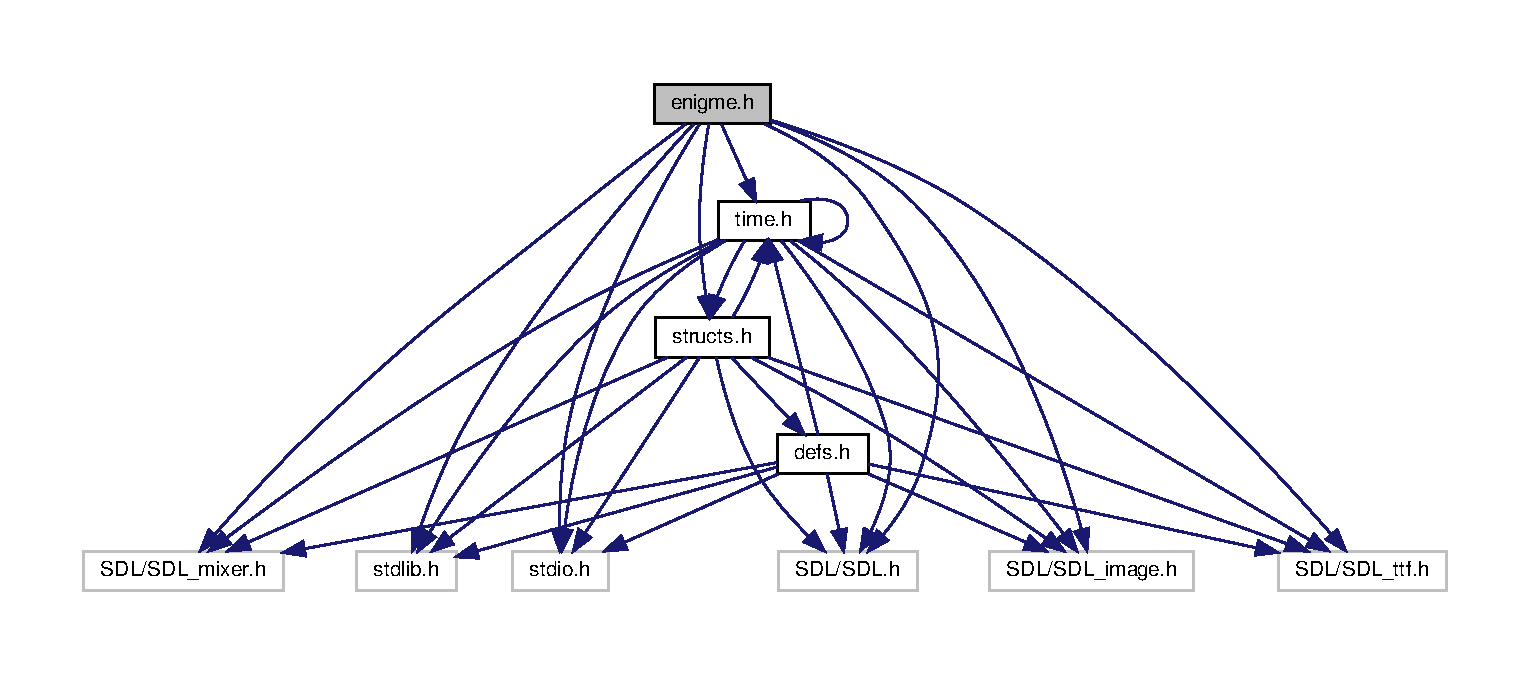
\includegraphics[width=350pt]{enigme_8h__incl}
\end{center}
\end{figure}
This graph shows which files directly or indirectly include this file\+:
\nopagebreak
\begin{figure}[H]
\begin{center}
\leavevmode
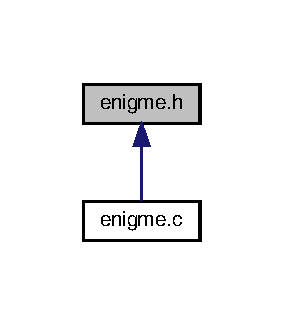
\includegraphics[width=136pt]{enigme_8h__dep__incl}
\end{center}
\end{figure}
\subsection*{Data Structures}
\begin{DoxyCompactItemize}
\item 
struct \hyperlink{structenigme}{enigme}
\end{DoxyCompactItemize}
\subsection*{Functions}
\begin{DoxyCompactItemize}
\item 
\mbox{\Hypertarget{enigme_8h_a194546ea4fa1a0eaa63aacbac96f33bb}\label{enigme_8h_a194546ea4fa1a0eaa63aacbac96f33bb}} 
void {\bfseries init\+\_\+enigme} (\hyperlink{structenigme}{enigme} $\ast$e)
\item 
\mbox{\Hypertarget{enigme_8h_a345b17b765ec6a985fb162957d6e900c}\label{enigme_8h_a345b17b765ec6a985fb162957d6e900c}} 
void {\bfseries generate\+\_\+afficher} (S\+D\+L\+\_\+\+Surface $\ast$screen, char image \mbox{[}$\,$\mbox{]}, \hyperlink{structenigme}{enigme} $\ast$e, int $\ast$alea)
\item 
\mbox{\Hypertarget{enigme_8h_a6754b2ea5ab28613588b0286e5b0ce4c}\label{enigme_8h_a6754b2ea5ab28613588b0286e5b0ce4c}} 
int {\bfseries solution} (char image \mbox{[}$\,$\mbox{]})
\item 
\mbox{\Hypertarget{enigme_8h_ae855a03b9d7f7619bac3843306965df9}\label{enigme_8h_ae855a03b9d7f7619bac3843306965df9}} 
int {\bfseries resolution} (int $\ast$running, int $\ast$run)
\item 
\mbox{\Hypertarget{enigme_8h_a4000acf4af9607e9d50a33b70643a99a}\label{enigme_8h_a4000acf4af9607e9d50a33b70643a99a}} 
void {\bfseries afficher\+\_\+resultat} (S\+D\+L\+\_\+\+Surface $\ast$screen, int s, int r, \hyperlink{structenigme}{enigme} $\ast$en)
\end{DoxyCompactItemize}
\subsection*{Variables}
\begin{DoxyCompactItemize}
\item 
\mbox{\Hypertarget{enigme_8h_abbeff4ee7b328d6b61b563ecded5bf83}\label{enigme_8h_abbeff4ee7b328d6b61b563ecded5bf83}} 
\hyperlink{structGestion}{Gestion} {\bfseries jeu}
\item 
\mbox{\Hypertarget{enigme_8h_a7a56ddcc26459f1d1b0391d1a2025448}\label{enigme_8h_a7a56ddcc26459f1d1b0391d1a2025448}} 
\hyperlink{structHero}{Hero} {\bfseries player}
\end{DoxyCompactItemize}


\subsection{Detailed Description}
enigme libs 

\begin{DoxyAuthor}{Author}
Raed+\+Youssef 
\end{DoxyAuthor}
\begin{DoxyVersion}{Version}
1.\+0 
\end{DoxyVersion}
\begin{DoxyDate}{Date}
07/06/2020 
\end{DoxyDate}

\hypertarget{font_8c}{}\section{font.\+c File Reference}
\label{font_8c}\index{font.\+c@{font.\+c}}


font libs  


{\ttfamily \#include $<$stdlib.\+h$>$}\newline
{\ttfamily \#include $<$stdio.\+h$>$}\newline
{\ttfamily \#include $<$S\+D\+L/\+S\+D\+L.\+h$>$}\newline
{\ttfamily \#include $<$S\+D\+L/\+S\+D\+L\+\_\+image.\+h$>$}\newline
{\ttfamily \#include $<$S\+D\+L/\+S\+D\+L\+\_\+mixer.\+h$>$}\newline
{\ttfamily \#include $<$S\+D\+L/\+S\+D\+L\+\_\+ttf.\+h$>$}\newline
{\ttfamily \#include $<$time.\+h$>$}\newline
{\ttfamily \#include \char`\"{}font.\+h\char`\"{}}\newline
Include dependency graph for font.\+c\+:
\nopagebreak
\begin{figure}[H]
\begin{center}
\leavevmode
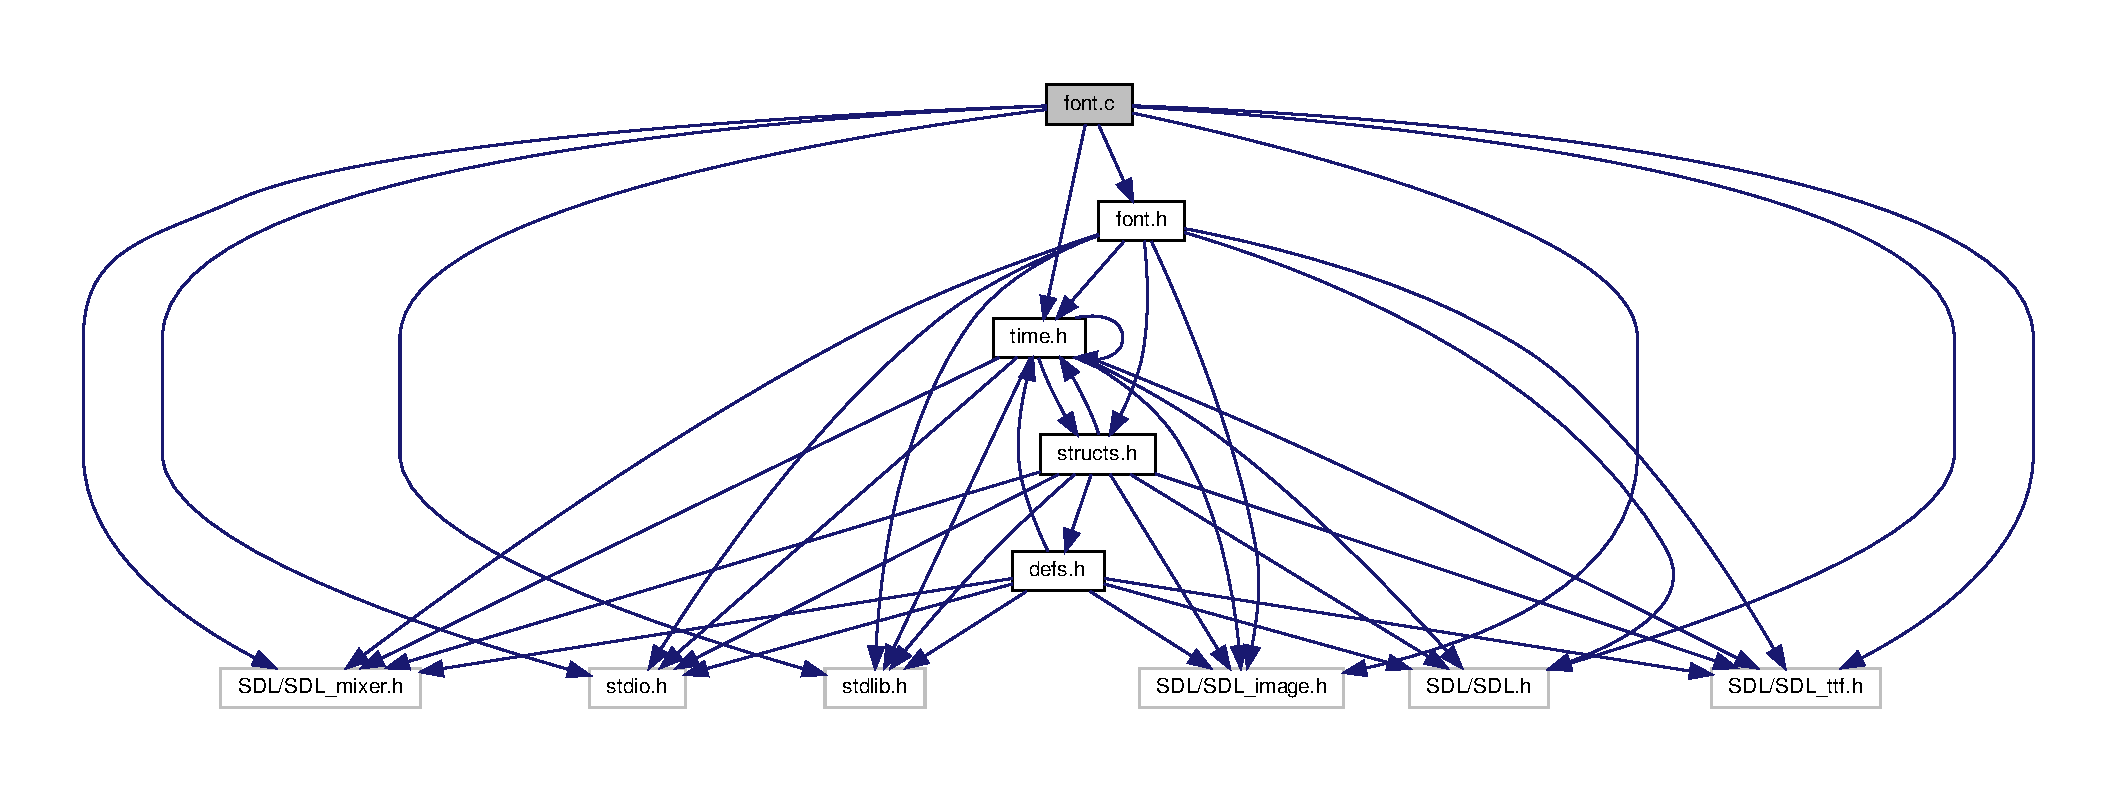
\includegraphics[width=350pt]{font_8c__incl}
\end{center}
\end{figure}
\subsection*{Functions}
\begin{DoxyCompactItemize}
\item 
\mbox{\Hypertarget{font_8c_afb80fbb72b2b7fd6a194084b64887074}\label{font_8c_afb80fbb72b2b7fd6a194084b64887074}} 
T\+T\+F\+\_\+\+Font $\ast$ {\bfseries load\+Font} (char $\ast$name, int size)
\item 
\mbox{\Hypertarget{font_8c_ad5586264a42819b567898cff66287f6e}\label{font_8c_ad5586264a42819b567898cff66287f6e}} 
void {\bfseries close\+Font} (T\+T\+F\+\_\+\+Font $\ast$font)
\item 
\mbox{\Hypertarget{font_8c_a83d0894aca32e4162ff85241c123286c}\label{font_8c_a83d0894aca32e4162ff85241c123286c}} 
void {\bfseries draw\+String} (char $\ast$text, int x, int y, T\+T\+F\+\_\+\+Font $\ast$font)
\item 
\mbox{\Hypertarget{font_8c_af646d273a1348946bb843f25e39a58bb}\label{font_8c_af646d273a1348946bb843f25e39a58bb}} 
void {\bfseries draw\+\_\+\+String} (char $\ast$text, int x, int y, T\+T\+F\+\_\+\+Font $\ast$font)
\end{DoxyCompactItemize}


\subsection{Detailed Description}
font libs 

\begin{DoxyAuthor}{Author}
Youssef 
\end{DoxyAuthor}
\begin{DoxyVersion}{Version}
1.\+0 
\end{DoxyVersion}
\begin{DoxyDate}{Date}
07/06/2020 
\end{DoxyDate}

\hypertarget{font_8h}{}\section{font.\+h File Reference}
\label{font_8h}\index{font.\+h@{font.\+h}}


font libs  


{\ttfamily \#include $<$stdlib.\+h$>$}\newline
{\ttfamily \#include $<$stdio.\+h$>$}\newline
{\ttfamily \#include $<$S\+D\+L/\+S\+D\+L.\+h$>$}\newline
{\ttfamily \#include $<$S\+D\+L/\+S\+D\+L\+\_\+image.\+h$>$}\newline
{\ttfamily \#include $<$S\+D\+L/\+S\+D\+L\+\_\+mixer.\+h$>$}\newline
{\ttfamily \#include $<$S\+D\+L/\+S\+D\+L\+\_\+ttf.\+h$>$}\newline
{\ttfamily \#include $<$time.\+h$>$}\newline
{\ttfamily \#include \char`\"{}structs.\+h\char`\"{}}\newline
Include dependency graph for font.\+h\+:
\nopagebreak
\begin{figure}[H]
\begin{center}
\leavevmode
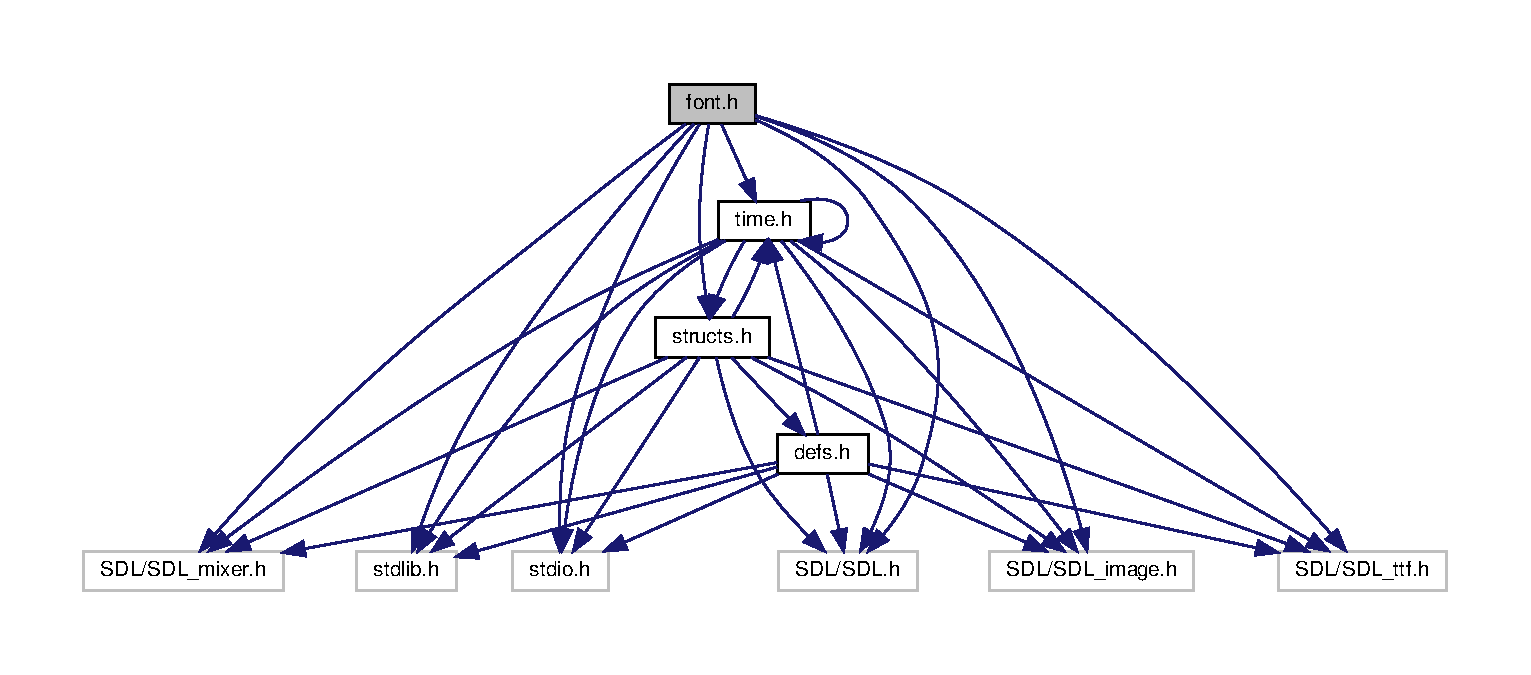
\includegraphics[width=350pt]{font_8h__incl}
\end{center}
\end{figure}
This graph shows which files directly or indirectly include this file\+:
\nopagebreak
\begin{figure}[H]
\begin{center}
\leavevmode
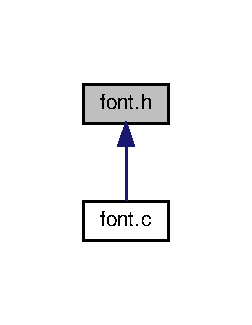
\includegraphics[width=121pt]{font_8h__dep__incl}
\end{center}
\end{figure}
\subsection*{Variables}
\begin{DoxyCompactItemize}
\item 
\mbox{\Hypertarget{font_8h_abbeff4ee7b328d6b61b563ecded5bf83}\label{font_8h_abbeff4ee7b328d6b61b563ecded5bf83}} 
\hyperlink{structGestion}{Gestion} {\bfseries jeu}
\item 
\mbox{\Hypertarget{font_8h_abf5bfa705e66ffc1ddaa6ce46c960873}\label{font_8h_abf5bfa705e66ffc1ddaa6ce46c960873}} 
T\+T\+F\+\_\+\+Font $\ast$ {\bfseries font}
\end{DoxyCompactItemize}


\subsection{Detailed Description}
font libs 

\begin{DoxyAuthor}{Author}
Youssef 
\end{DoxyAuthor}
\begin{DoxyVersion}{Version}
1.\+0 
\end{DoxyVersion}
\begin{DoxyDate}{Date}
07/06/2020 
\end{DoxyDate}

\hypertarget{init_8c}{}\section{init.\+c File Reference}
\label{init_8c}\index{init.\+c@{init.\+c}}


init libs  


{\ttfamily \#include $<$stdlib.\+h$>$}\newline
{\ttfamily \#include $<$stdio.\+h$>$}\newline
{\ttfamily \#include $<$S\+D\+L/\+S\+D\+L.\+h$>$}\newline
{\ttfamily \#include $<$S\+D\+L/\+S\+D\+L\+\_\+image.\+h$>$}\newline
{\ttfamily \#include $<$S\+D\+L/\+S\+D\+L\+\_\+mixer.\+h$>$}\newline
{\ttfamily \#include $<$S\+D\+L/\+S\+D\+L\+\_\+ttf.\+h$>$}\newline
{\ttfamily \#include $<$time.\+h$>$}\newline
{\ttfamily \#include \char`\"{}init.\+h\char`\"{}}\newline
Include dependency graph for init.\+c\+:
\nopagebreak
\begin{figure}[H]
\begin{center}
\leavevmode
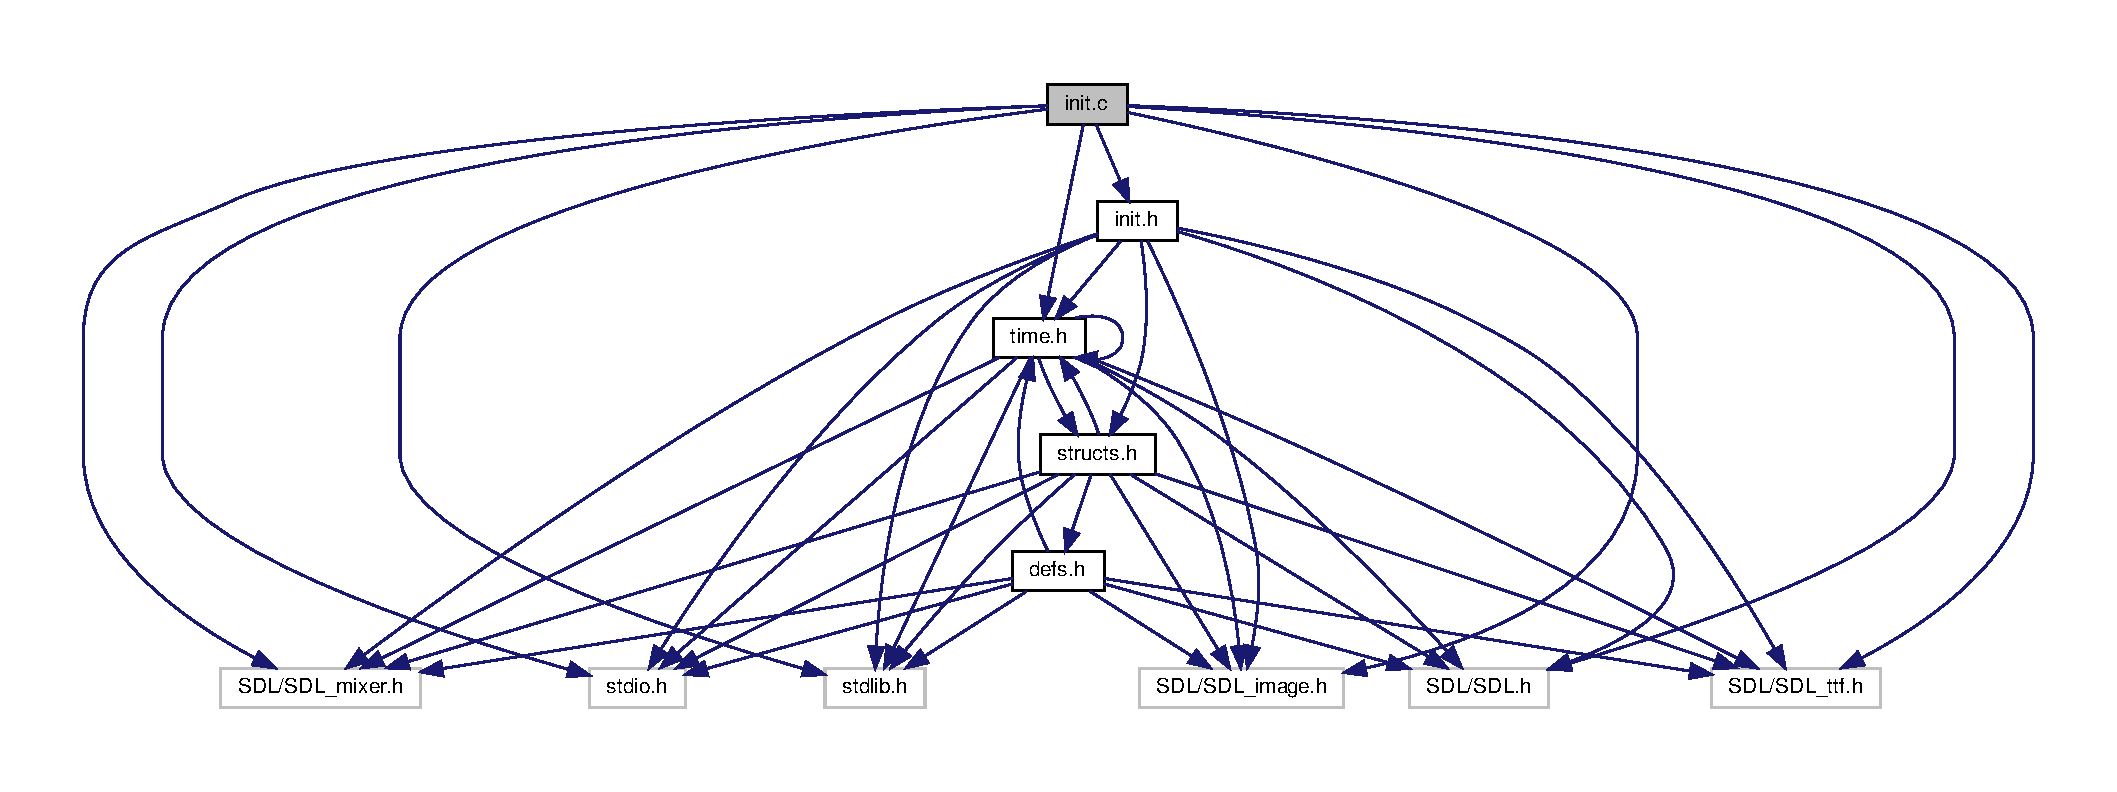
\includegraphics[width=350pt]{init_8c__incl}
\end{center}
\end{figure}
\subsection*{Functions}
\begin{DoxyCompactItemize}
\item 
\mbox{\Hypertarget{init_8c_a4625abbd174dfbdfec9f4cf9124217a8}\label{init_8c_a4625abbd174dfbdfec9f4cf9124217a8}} 
void {\bfseries init} (char $\ast$title)
\item 
\mbox{\Hypertarget{init_8c_a793872fec0a901ff46e527d3811fc6b9}\label{init_8c_a793872fec0a901ff46e527d3811fc6b9}} 
void {\bfseries load\+Game} (void)
\item 
\mbox{\Hypertarget{init_8c_a4b66d5e31b5dc18b314c8a68163263bd}\label{init_8c_a4b66d5e31b5dc18b314c8a68163263bd}} 
void {\bfseries cleanup} ()
\end{DoxyCompactItemize}


\subsection{Detailed Description}
init libs 

\begin{DoxyAuthor}{Author}
Youssef+\+Cyrine 
\end{DoxyAuthor}
\begin{DoxyVersion}{Version}
1.\+0 
\end{DoxyVersion}
\begin{DoxyDate}{Date}
07/06/2020 
\end{DoxyDate}

\hypertarget{init_8h}{}\section{init.\+h File Reference}
\label{init_8h}\index{init.\+h@{init.\+h}}


init libs  


{\ttfamily \#include $<$stdlib.\+h$>$}\newline
{\ttfamily \#include $<$stdio.\+h$>$}\newline
{\ttfamily \#include $<$S\+D\+L/\+S\+D\+L.\+h$>$}\newline
{\ttfamily \#include $<$S\+D\+L/\+S\+D\+L\+\_\+image.\+h$>$}\newline
{\ttfamily \#include $<$S\+D\+L/\+S\+D\+L\+\_\+mixer.\+h$>$}\newline
{\ttfamily \#include $<$S\+D\+L/\+S\+D\+L\+\_\+ttf.\+h$>$}\newline
{\ttfamily \#include $<$time.\+h$>$}\newline
{\ttfamily \#include \char`\"{}structs.\+h\char`\"{}}\newline
Include dependency graph for init.\+h\+:
\nopagebreak
\begin{figure}[H]
\begin{center}
\leavevmode
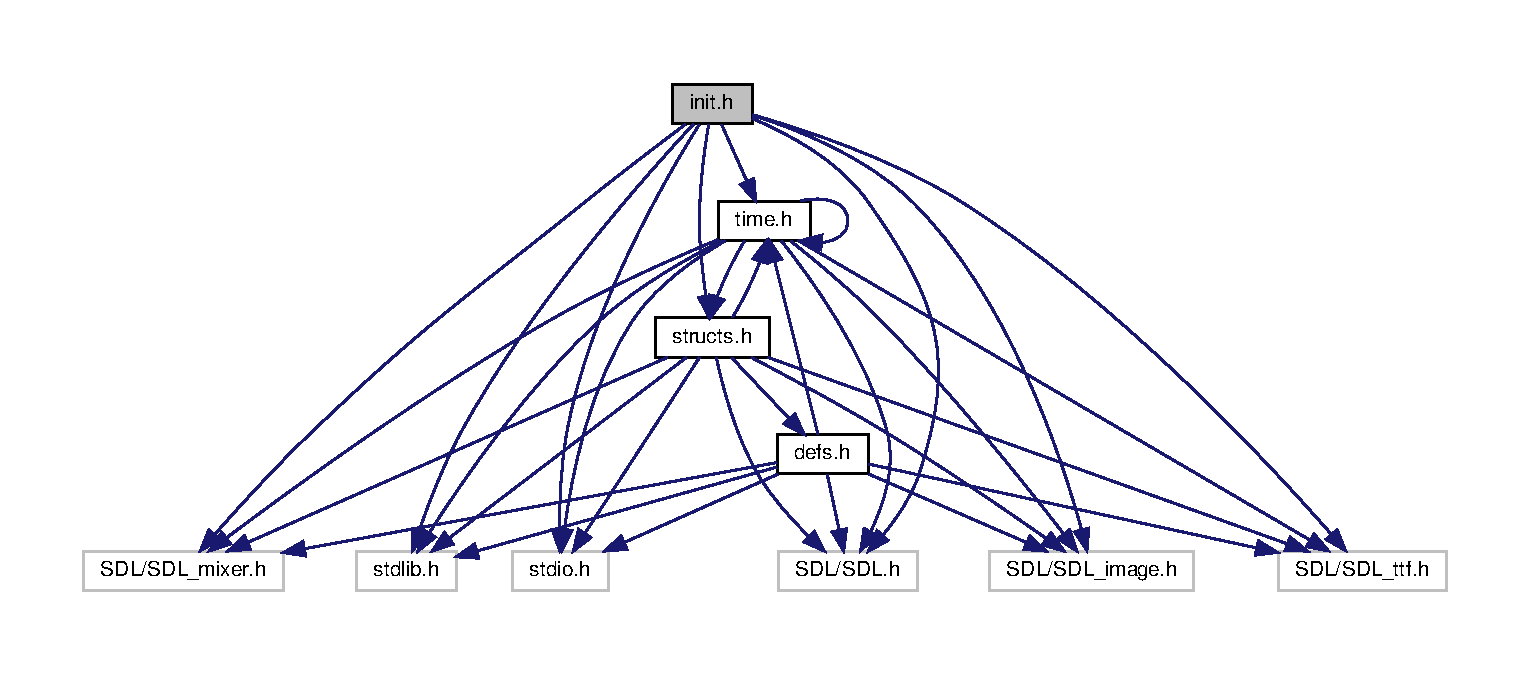
\includegraphics[width=350pt]{init_8h__incl}
\end{center}
\end{figure}
This graph shows which files directly or indirectly include this file\+:
\nopagebreak
\begin{figure}[H]
\begin{center}
\leavevmode
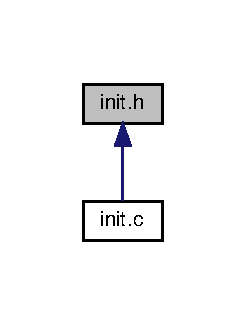
\includegraphics[width=118pt]{init_8h__dep__incl}
\end{center}
\end{figure}
\subsection*{Functions}
\begin{DoxyCompactItemize}
\item 
\mbox{\Hypertarget{init_8h_a12b9f50e1f51a4019b2b5cb8c8ed04b8}\label{init_8h_a12b9f50e1f51a4019b2b5cb8c8ed04b8}} 
S\+D\+L\+\_\+\+Surface $\ast$ {\bfseries load\+Image} (char $\ast$name)
\item 
\mbox{\Hypertarget{init_8h_ad5586264a42819b567898cff66287f6e}\label{init_8h_ad5586264a42819b567898cff66287f6e}} 
void {\bfseries close\+Font} (T\+T\+F\+\_\+\+Font $\ast$font)
\item 
\mbox{\Hypertarget{init_8h_af3ccec8743c190a3fbf6b83d1b3b65c8}\label{init_8h_af3ccec8743c190a3fbf6b83d1b3b65c8}} 
T\+T\+F\+\_\+\+Font $\ast$ {\bfseries load\+Font} (char $\ast$, int)
\item 
\mbox{\Hypertarget{init_8h_a1c001a82cba133dd3beb5ff6a014a537}\label{init_8h_a1c001a82cba133dd3beb5ff6a014a537}} 
void {\bfseries load\+Song} (char filename\mbox{[}200\mbox{]})
\item 
\mbox{\Hypertarget{init_8h_a86eb94e3b6f2b5b7c798dc02b0935500}\label{init_8h_a86eb94e3b6f2b5b7c798dc02b0935500}} 
void {\bfseries load\+Sound} (void)
\item 
\mbox{\Hypertarget{init_8h_afed923638f1c2eebd978b79bf62c5919}\label{init_8h_afed923638f1c2eebd978b79bf62c5919}} 
void {\bfseries free\+Sound} (void)
\end{DoxyCompactItemize}
\subsection*{Variables}
\begin{DoxyCompactItemize}
\item 
\mbox{\Hypertarget{init_8h_abbeff4ee7b328d6b61b563ecded5bf83}\label{init_8h_abbeff4ee7b328d6b61b563ecded5bf83}} 
\hyperlink{structGestion}{Gestion} {\bfseries jeu}
\item 
\mbox{\Hypertarget{init_8h_a32175bc9c482ed465d43f3e1d31f72a4}\label{init_8h_a32175bc9c482ed465d43f3e1d31f72a4}} 
\hyperlink{structGameobject}{Gameobject} {\bfseries star}
\item 
\mbox{\Hypertarget{init_8h_a7a56ddcc26459f1d1b0391d1a2025448}\label{init_8h_a7a56ddcc26459f1d1b0391d1a2025448}} 
\hyperlink{structHero}{Hero} {\bfseries player}
\item 
\mbox{\Hypertarget{init_8h_a2737dcd286631af70eac9ebd6de78a07}\label{init_8h_a2737dcd286631af70eac9ebd6de78a07}} 
\hyperlink{structHero}{Hero} {\bfseries monster}
\item 
\mbox{\Hypertarget{init_8h_ac9becb8e2f80125547c8cc8f9d56b7ab}\label{init_8h_ac9becb8e2f80125547c8cc8f9d56b7ab}} 
\hyperlink{structMap}{Map} {\bfseries map}
\item 
\mbox{\Hypertarget{init_8h_abf5bfa705e66ffc1ddaa6ce46c960873}\label{init_8h_abf5bfa705e66ffc1ddaa6ce46c960873}} 
T\+T\+F\+\_\+\+Font $\ast$ {\bfseries font}
\end{DoxyCompactItemize}


\subsection{Detailed Description}
init libs 

\begin{DoxyAuthor}{Author}
Youssef+\+Cyrine 
\end{DoxyAuthor}
\begin{DoxyVersion}{Version}
1.\+0 
\end{DoxyVersion}
\begin{DoxyDate}{Date}
07/06/2020 
\end{DoxyDate}

\hypertarget{input_8c}{}\section{input.\+c File Reference}
\label{input_8c}\index{input.\+c@{input.\+c}}


input libs  


{\ttfamily \#include $<$stdlib.\+h$>$}\newline
{\ttfamily \#include $<$stdio.\+h$>$}\newline
{\ttfamily \#include $<$S\+D\+L/\+S\+D\+L.\+h$>$}\newline
{\ttfamily \#include $<$S\+D\+L/\+S\+D\+L\+\_\+image.\+h$>$}\newline
{\ttfamily \#include $<$S\+D\+L/\+S\+D\+L\+\_\+mixer.\+h$>$}\newline
{\ttfamily \#include $<$S\+D\+L/\+S\+D\+L\+\_\+ttf.\+h$>$}\newline
{\ttfamily \#include $<$time.\+h$>$}\newline
{\ttfamily \#include \char`\"{}input.\+h\char`\"{}}\newline
Include dependency graph for input.\+c\+:
\nopagebreak
\begin{figure}[H]
\begin{center}
\leavevmode
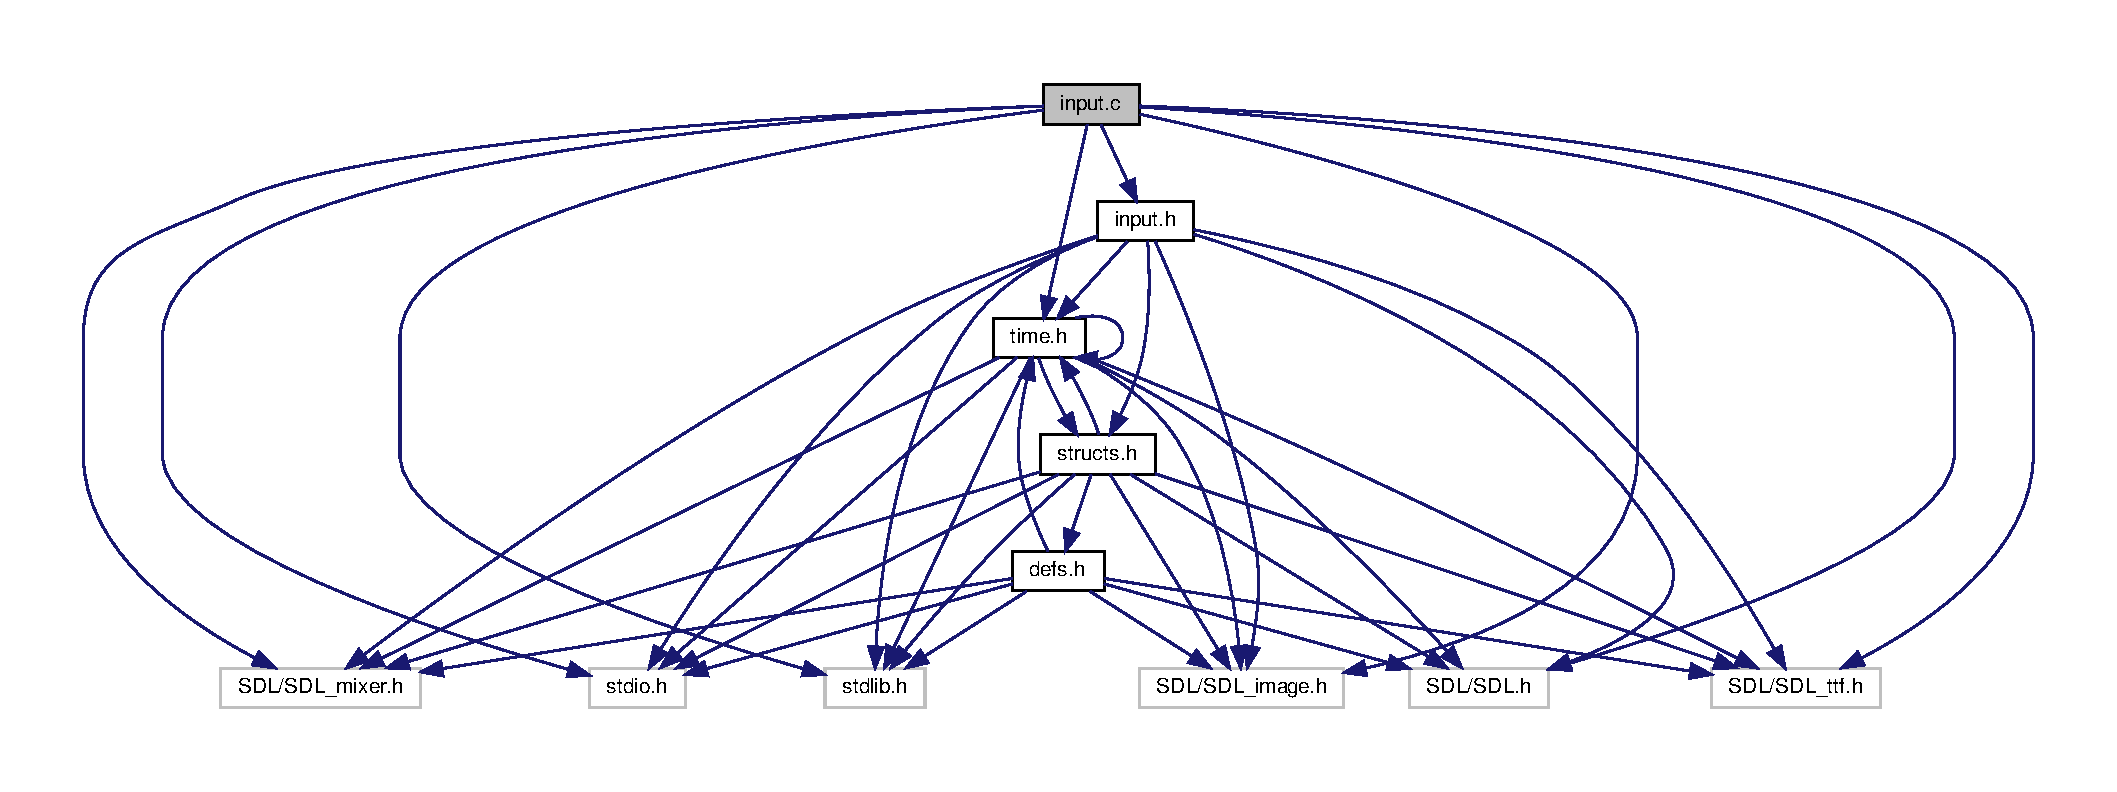
\includegraphics[width=350pt]{input_8c__incl}
\end{center}
\end{figure}
\subsection*{Functions}
\begin{DoxyCompactItemize}
\item 
\mbox{\Hypertarget{input_8c_a46d47190cb20b54826fb665f1859968f}\label{input_8c_a46d47190cb20b54826fb665f1859968f}} 
void {\bfseries get\+Input} ()
\item 
\mbox{\Hypertarget{input_8c_a0281b2ab36f3128172d50fabec311fe6}\label{input_8c_a0281b2ab36f3128172d50fabec311fe6}} 
void {\bfseries get\+Joystick} ()
\end{DoxyCompactItemize}


\subsection{Detailed Description}
input libs 

\begin{DoxyAuthor}{Author}
Youssef+\+Cyrine 
\end{DoxyAuthor}
\begin{DoxyVersion}{Version}
1.\+0 
\end{DoxyVersion}
\begin{DoxyDate}{Date}
07/06/2020 
\end{DoxyDate}

\hypertarget{input_8h}{}\section{input.\+h File Reference}
\label{input_8h}\index{input.\+h@{input.\+h}}


input libs  


{\ttfamily \#include $<$stdlib.\+h$>$}\newline
{\ttfamily \#include $<$stdio.\+h$>$}\newline
{\ttfamily \#include $<$S\+D\+L/\+S\+D\+L.\+h$>$}\newline
{\ttfamily \#include $<$S\+D\+L/\+S\+D\+L\+\_\+image.\+h$>$}\newline
{\ttfamily \#include $<$S\+D\+L/\+S\+D\+L\+\_\+mixer.\+h$>$}\newline
{\ttfamily \#include $<$S\+D\+L/\+S\+D\+L\+\_\+ttf.\+h$>$}\newline
{\ttfamily \#include $<$time.\+h$>$}\newline
{\ttfamily \#include \char`\"{}structs.\+h\char`\"{}}\newline
Include dependency graph for input.\+h\+:
\nopagebreak
\begin{figure}[H]
\begin{center}
\leavevmode
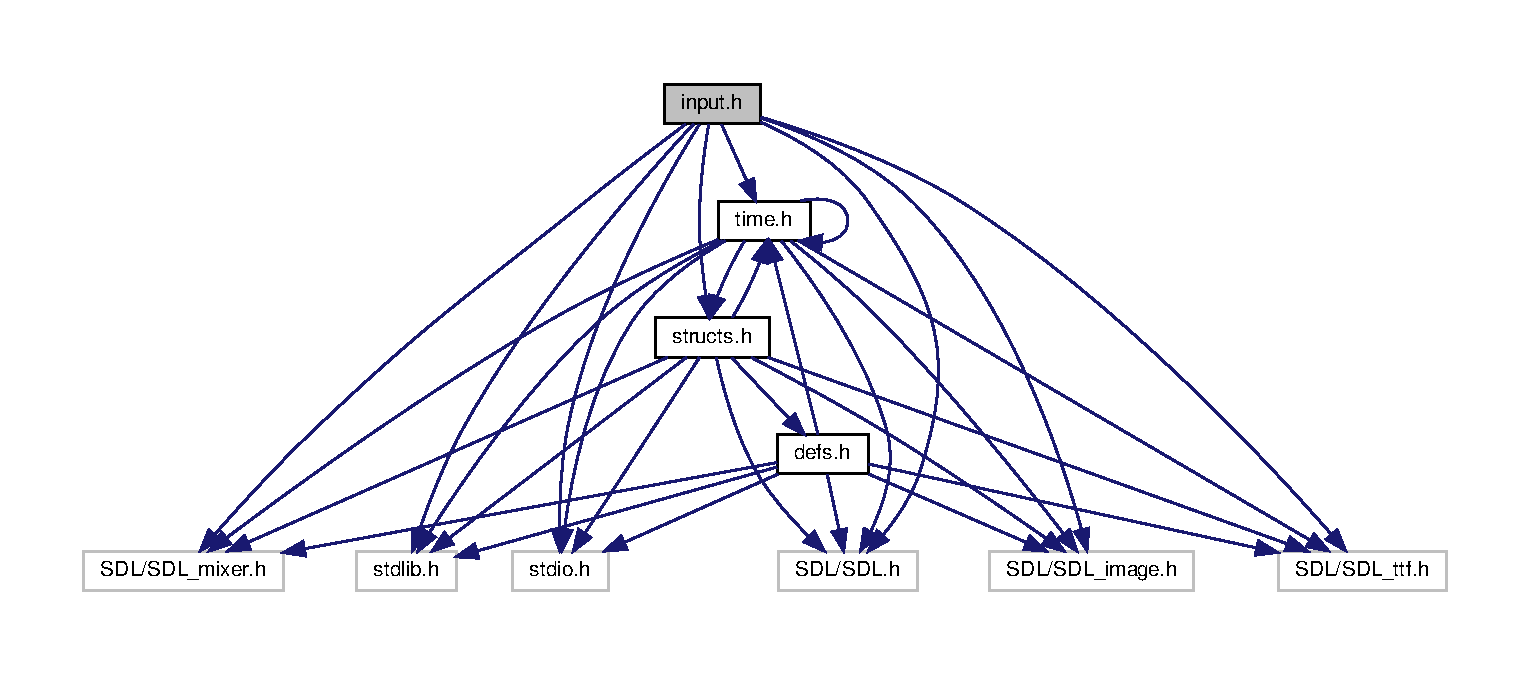
\includegraphics[width=350pt]{input_8h__incl}
\end{center}
\end{figure}
This graph shows which files directly or indirectly include this file\+:
\nopagebreak
\begin{figure}[H]
\begin{center}
\leavevmode
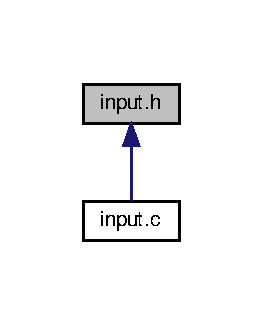
\includegraphics[width=126pt]{input_8h__dep__incl}
\end{center}
\end{figure}
\subsection*{Variables}
\begin{DoxyCompactItemize}
\item 
\mbox{\Hypertarget{input_8h_ad4db59ccea8946af2bb70f8269e99eeb}\label{input_8h_ad4db59ccea8946af2bb70f8269e99eeb}} 
\hyperlink{structInput}{Input} {\bfseries input}
\item 
\mbox{\Hypertarget{input_8h_abbeff4ee7b328d6b61b563ecded5bf83}\label{input_8h_abbeff4ee7b328d6b61b563ecded5bf83}} 
\hyperlink{structGestion}{Gestion} {\bfseries jeu}
\item 
\mbox{\Hypertarget{input_8h_a7e63f9e6912e012279f8c1c5bd884bb2}\label{input_8h_a7e63f9e6912e012279f8c1c5bd884bb2}} 
int {\bfseries D\+P\+A\+Din\+Use} = 0
\end{DoxyCompactItemize}


\subsection{Detailed Description}
input libs 

\begin{DoxyAuthor}{Author}
Youssef+\+Cyrine 
\end{DoxyAuthor}
\begin{DoxyVersion}{Version}
1.\+0 
\end{DoxyVersion}
\begin{DoxyDate}{Date}
07/06/2020 
\end{DoxyDate}

\hypertarget{jump_8c}{}\section{jump.\+c File Reference}
\label{jump_8c}\index{jump.\+c@{jump.\+c}}


jump libs  


{\ttfamily \#include $<$stdlib.\+h$>$}\newline
{\ttfamily \#include $<$stdio.\+h$>$}\newline
{\ttfamily \#include $<$S\+D\+L/\+S\+D\+L.\+h$>$}\newline
{\ttfamily \#include $<$S\+D\+L/\+S\+D\+L\+\_\+image.\+h$>$}\newline
{\ttfamily \#include $<$S\+D\+L/\+S\+D\+L\+\_\+mixer.\+h$>$}\newline
{\ttfamily \#include $<$S\+D\+L/\+S\+D\+L\+\_\+ttf.\+h$>$}\newline
{\ttfamily \#include $<$time.\+h$>$}\newline
{\ttfamily \#include \char`\"{}jump.\+h\char`\"{}}\newline
Include dependency graph for jump.\+c\+:
\nopagebreak
\begin{figure}[H]
\begin{center}
\leavevmode
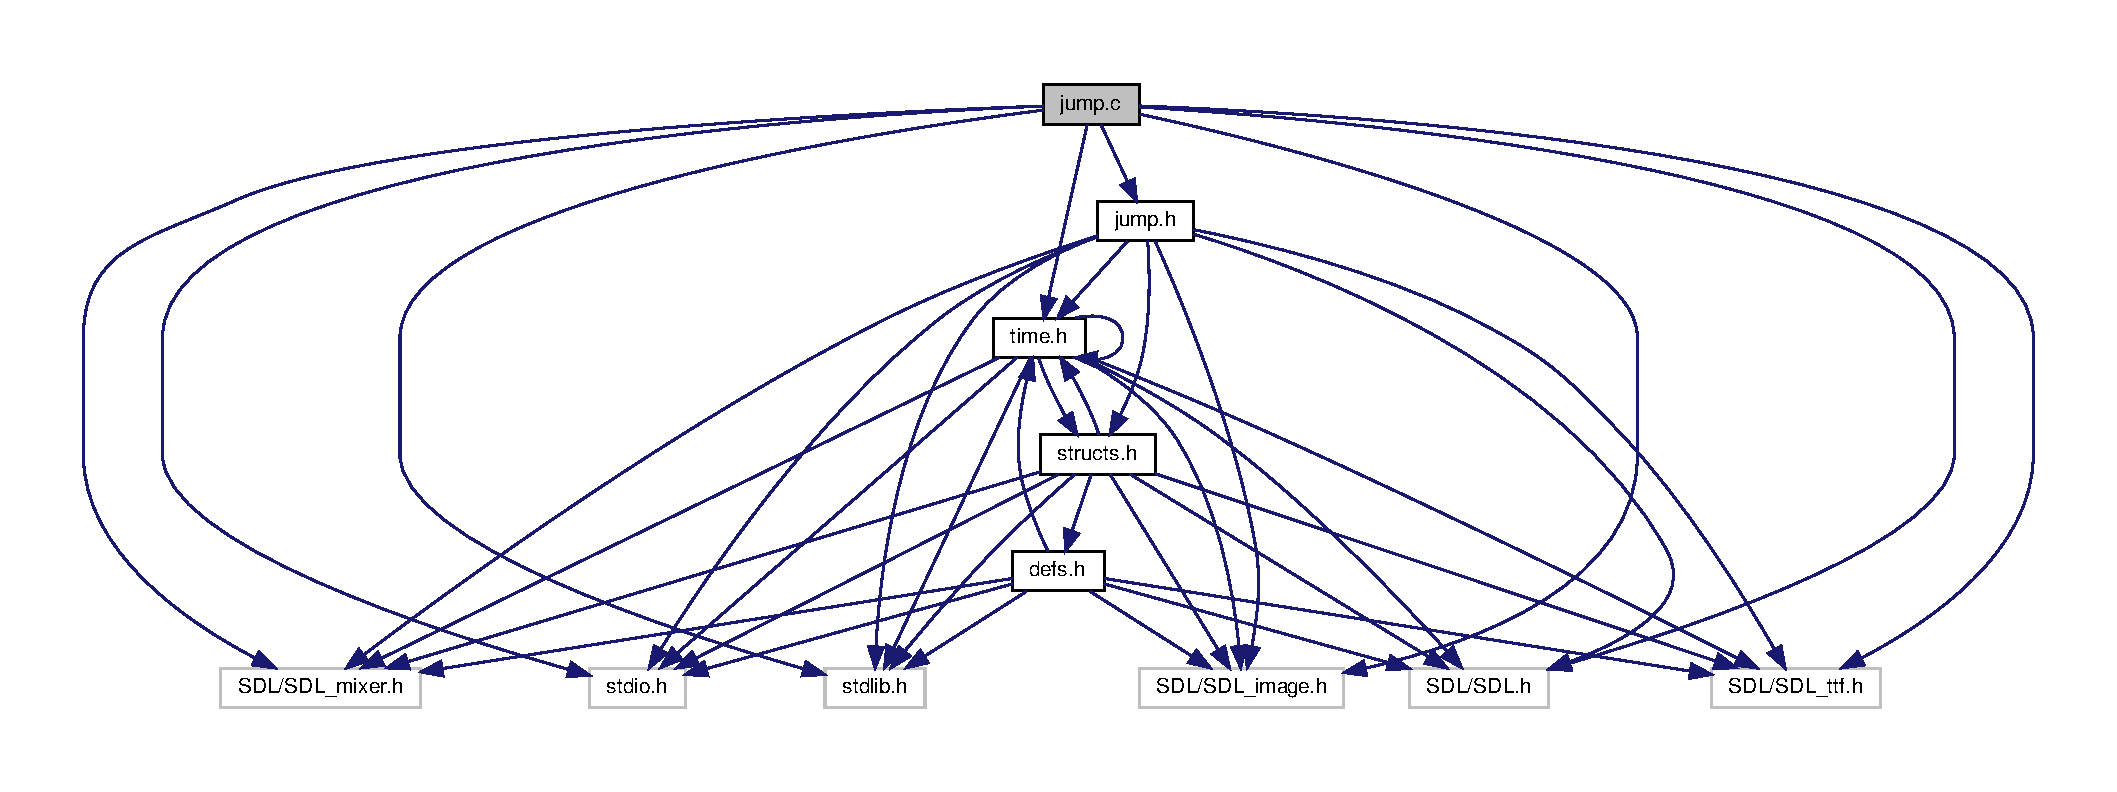
\includegraphics[width=350pt]{jump_8c__incl}
\end{center}
\end{figure}
\subsection*{Functions}
\begin{DoxyCompactItemize}
\item 
\mbox{\Hypertarget{jump_8c_aa9dab8db76b8b6eb581de87b277e142a}\label{jump_8c_aa9dab8db76b8b6eb581de87b277e142a}} 
void {\bfseries jump} (void)
\end{DoxyCompactItemize}


\subsection{Detailed Description}
jump libs 

\begin{DoxyAuthor}{Author}
Yasmine 
\end{DoxyAuthor}
\begin{DoxyVersion}{Version}
1.\+0 
\end{DoxyVersion}
\begin{DoxyDate}{Date}
07/06/2020 
\end{DoxyDate}

\hypertarget{jump_8h}{}\section{jump.\+h File Reference}
\label{jump_8h}\index{jump.\+h@{jump.\+h}}


jump libs  


{\ttfamily \#include $<$stdlib.\+h$>$}\newline
{\ttfamily \#include $<$stdio.\+h$>$}\newline
{\ttfamily \#include $<$S\+D\+L/\+S\+D\+L.\+h$>$}\newline
{\ttfamily \#include $<$S\+D\+L/\+S\+D\+L\+\_\+image.\+h$>$}\newline
{\ttfamily \#include $<$S\+D\+L/\+S\+D\+L\+\_\+mixer.\+h$>$}\newline
{\ttfamily \#include $<$S\+D\+L/\+S\+D\+L\+\_\+ttf.\+h$>$}\newline
{\ttfamily \#include $<$time.\+h$>$}\newline
{\ttfamily \#include \char`\"{}structs.\+h\char`\"{}}\newline
Include dependency graph for jump.\+h\+:
\nopagebreak
\begin{figure}[H]
\begin{center}
\leavevmode
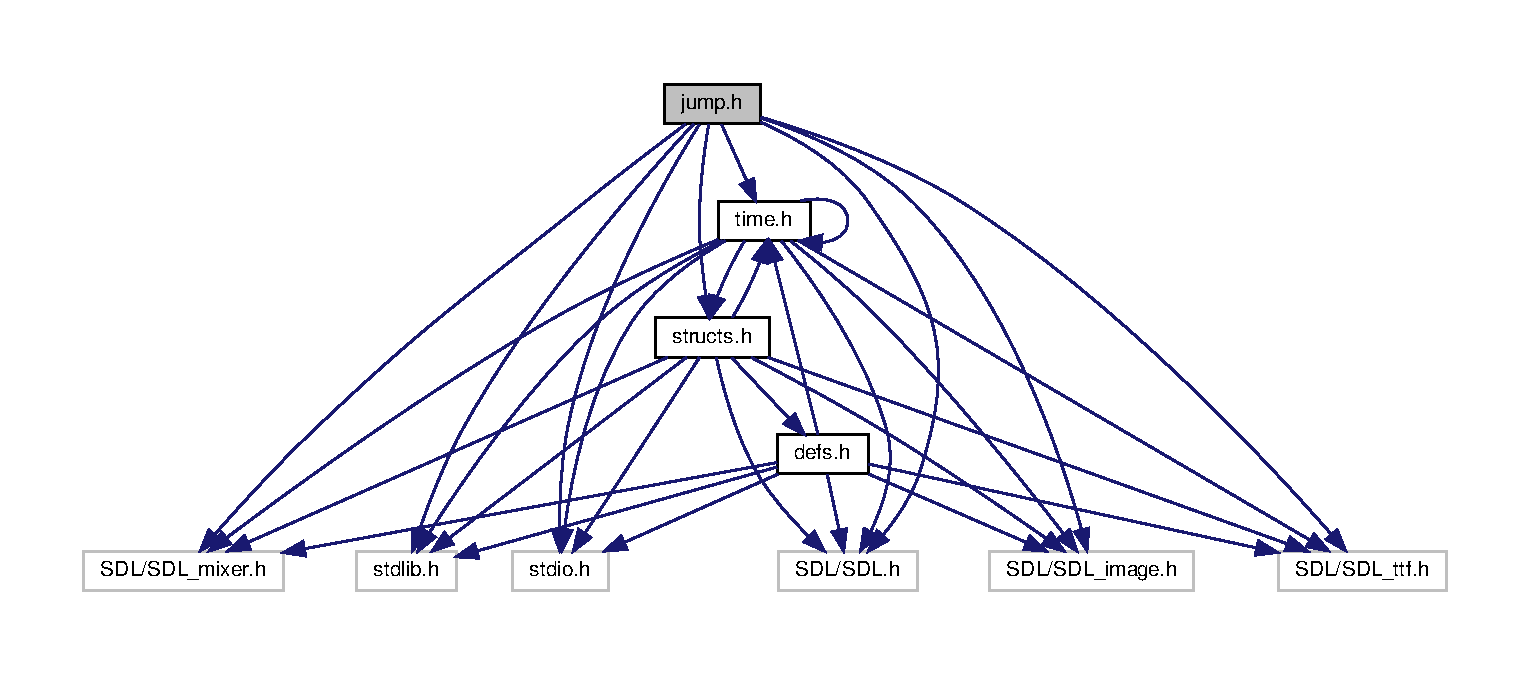
\includegraphics[width=350pt]{jump_8h__incl}
\end{center}
\end{figure}
This graph shows which files directly or indirectly include this file\+:
\nopagebreak
\begin{figure}[H]
\begin{center}
\leavevmode
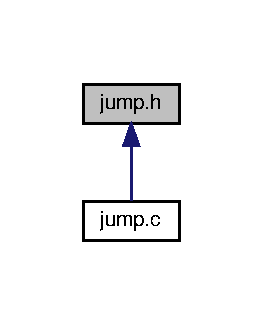
\includegraphics[width=126pt]{jump_8h__dep__incl}
\end{center}
\end{figure}
\subsection*{Functions}
\begin{DoxyCompactItemize}
\item 
\mbox{\Hypertarget{jump_8h_aa9dab8db76b8b6eb581de87b277e142a}\label{jump_8h_aa9dab8db76b8b6eb581de87b277e142a}} 
void {\bfseries jump} (void)
\end{DoxyCompactItemize}
\subsection*{Variables}
\begin{DoxyCompactItemize}
\item 
\mbox{\Hypertarget{jump_8h_a7a56ddcc26459f1d1b0391d1a2025448}\label{jump_8h_a7a56ddcc26459f1d1b0391d1a2025448}} 
\hyperlink{structHero}{Hero} {\bfseries player}
\item 
\mbox{\Hypertarget{jump_8h_ad4db59ccea8946af2bb70f8269e99eeb}\label{jump_8h_ad4db59ccea8946af2bb70f8269e99eeb}} 
\hyperlink{structInput}{Input} {\bfseries input}
\item 
\mbox{\Hypertarget{jump_8h_abbeff4ee7b328d6b61b563ecded5bf83}\label{jump_8h_abbeff4ee7b328d6b61b563ecded5bf83}} 
\hyperlink{structGestion}{Gestion} {\bfseries jeu}
\end{DoxyCompactItemize}


\subsection{Detailed Description}
jump libs 

\begin{DoxyAuthor}{Author}
Yasmine 
\end{DoxyAuthor}
\begin{DoxyVersion}{Version}
1.\+0 
\end{DoxyVersion}
\begin{DoxyDate}{Date}
07/06/2020 
\end{DoxyDate}

\hypertarget{main_8c}{}\section{main.\+c File Reference}
\label{main_8c}\index{main.\+c@{main.\+c}}


main libs  


{\ttfamily \#include $<$stdlib.\+h$>$}\newline
{\ttfamily \#include $<$stdio.\+h$>$}\newline
{\ttfamily \#include $<$S\+D\+L/\+S\+D\+L.\+h$>$}\newline
{\ttfamily \#include $<$S\+D\+L/\+S\+D\+L\+\_\+image.\+h$>$}\newline
{\ttfamily \#include $<$S\+D\+L/\+S\+D\+L\+\_\+mixer.\+h$>$}\newline
{\ttfamily \#include $<$S\+D\+L/\+S\+D\+L\+\_\+ttf.\+h$>$}\newline
{\ttfamily \#include $<$time.\+h$>$}\newline
{\ttfamily \#include \char`\"{}main.\+h\char`\"{}}\newline
Include dependency graph for main.\+c\+:
\nopagebreak
\begin{figure}[H]
\begin{center}
\leavevmode
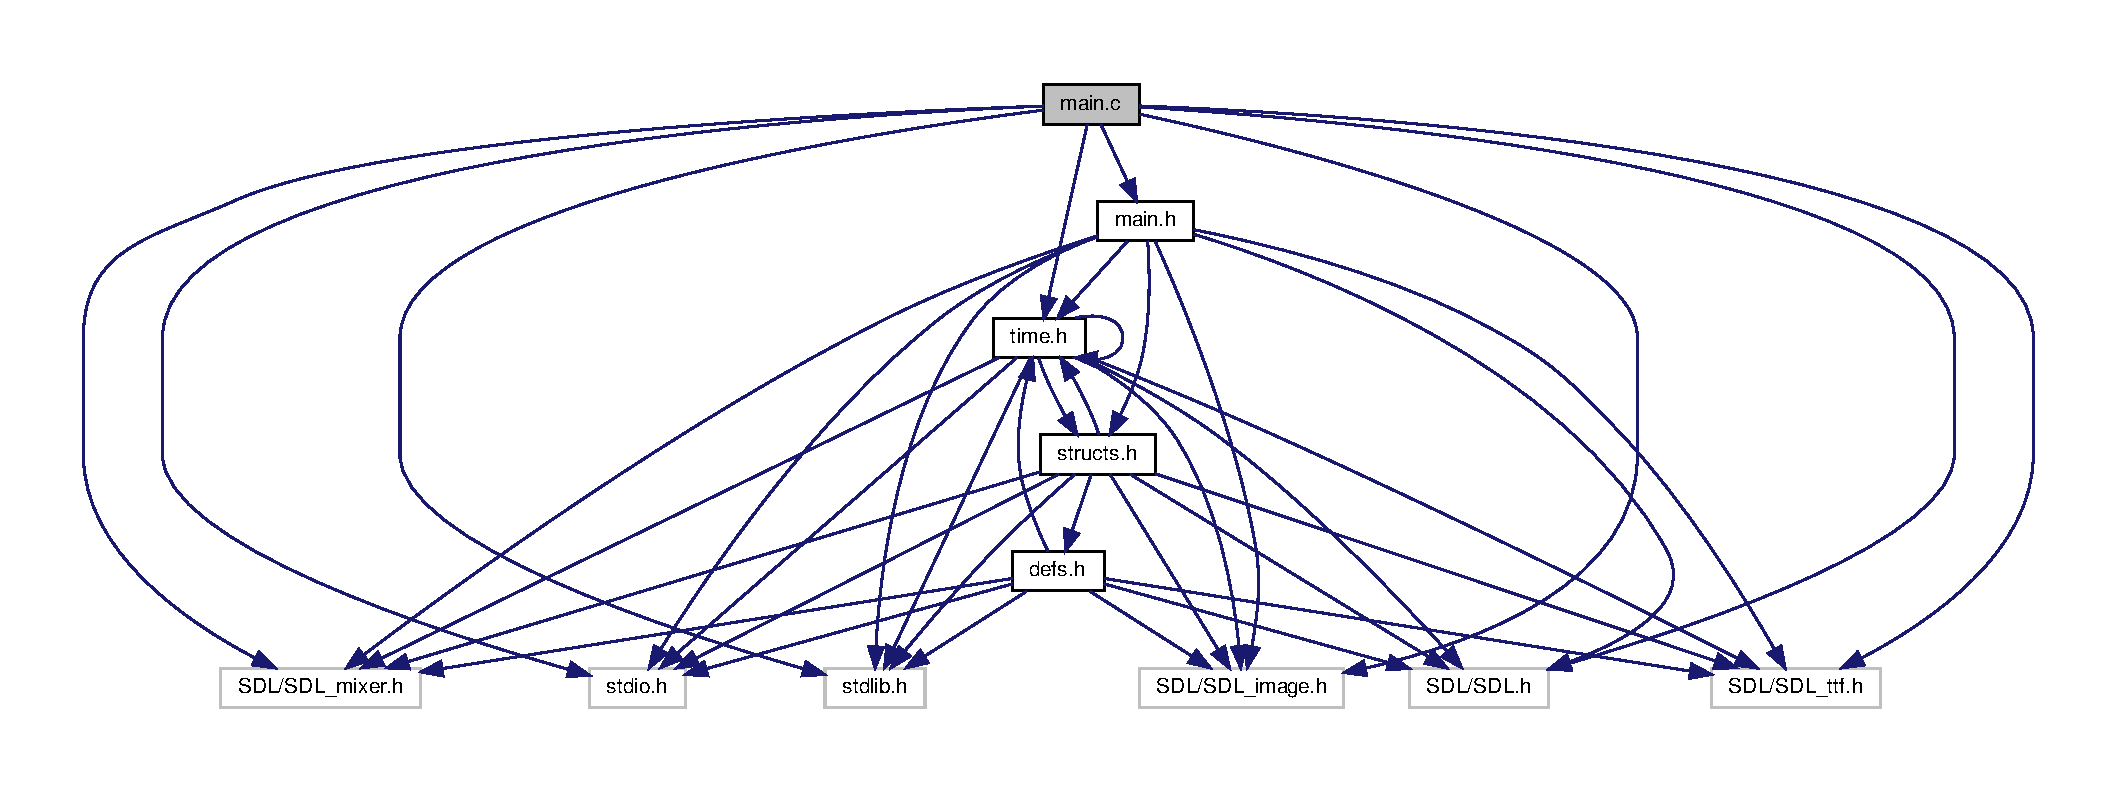
\includegraphics[width=350pt]{main_8c__incl}
\end{center}
\end{figure}
\subsection*{Functions}
\begin{DoxyCompactItemize}
\item 
\mbox{\Hypertarget{main_8c_a0ddf1224851353fc92bfbff6f499fa97}\label{main_8c_a0ddf1224851353fc92bfbff6f499fa97}} 
int {\bfseries main} (int argc, char $\ast$argv\mbox{[}$\,$\mbox{]})
\end{DoxyCompactItemize}


\subsection{Detailed Description}
main libs 

\begin{DoxyAuthor}{Author}
Dynamic 
\end{DoxyAuthor}
\begin{DoxyVersion}{Version}
1.\+0 
\end{DoxyVersion}
\begin{DoxyDate}{Date}
07/06/2020 
\end{DoxyDate}

\hypertarget{main_8h}{}\section{main.\+h File Reference}
\label{main_8h}\index{main.\+h@{main.\+h}}


main libs  


{\ttfamily \#include $<$stdlib.\+h$>$}\newline
{\ttfamily \#include $<$stdio.\+h$>$}\newline
{\ttfamily \#include $<$S\+D\+L/\+S\+D\+L.\+h$>$}\newline
{\ttfamily \#include $<$S\+D\+L/\+S\+D\+L\+\_\+image.\+h$>$}\newline
{\ttfamily \#include $<$S\+D\+L/\+S\+D\+L\+\_\+mixer.\+h$>$}\newline
{\ttfamily \#include $<$S\+D\+L/\+S\+D\+L\+\_\+ttf.\+h$>$}\newline
{\ttfamily \#include $<$time.\+h$>$}\newline
{\ttfamily \#include \char`\"{}structs.\+h\char`\"{}}\newline
Include dependency graph for main.\+h\+:
\nopagebreak
\begin{figure}[H]
\begin{center}
\leavevmode
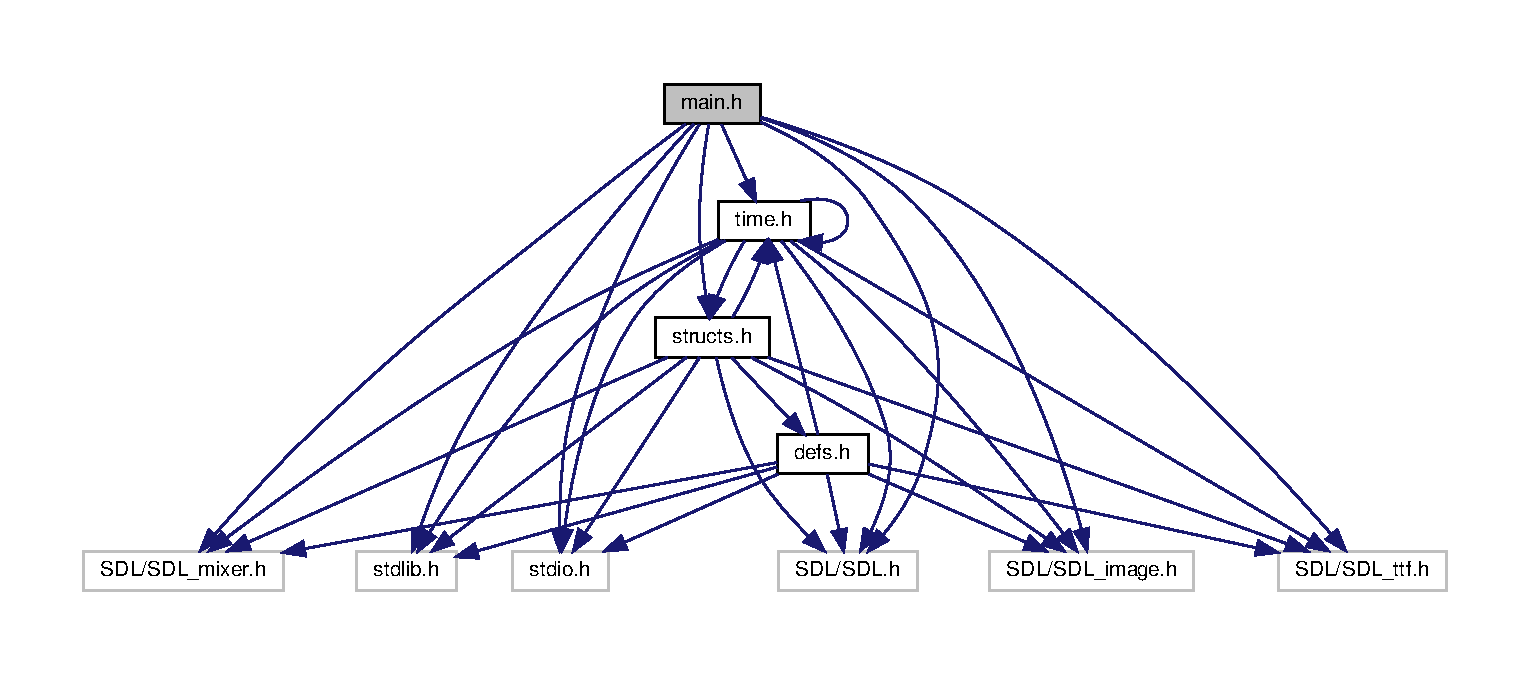
\includegraphics[width=350pt]{main_8h__incl}
\end{center}
\end{figure}
This graph shows which files directly or indirectly include this file\+:
\nopagebreak
\begin{figure}[H]
\begin{center}
\leavevmode
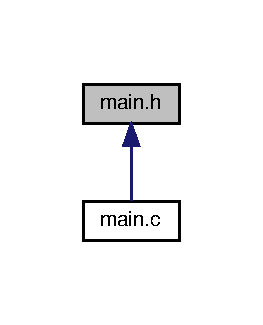
\includegraphics[width=126pt]{main_8h__dep__incl}
\end{center}
\end{figure}
\subsection*{Functions}
\begin{DoxyCompactItemize}
\item 
\mbox{\Hypertarget{main_8h_a8c3ce793e9c1aa17f38ac897502e5a3a}\label{main_8h_a8c3ce793e9c1aa17f38ac897502e5a3a}} 
void {\bfseries init} (char $\ast$)
\item 
\mbox{\Hypertarget{main_8h_aeb94fbd457627182ceee7e505f432541}\label{main_8h_aeb94fbd457627182ceee7e505f432541}} 
void {\bfseries cleanup} (void)
\item 
\mbox{\Hypertarget{main_8h_ada0e95826da8610f77df918d7c782cf0}\label{main_8h_ada0e95826da8610f77df918d7c782cf0}} 
void {\bfseries get\+Input} (void)
\item 
\mbox{\Hypertarget{main_8h_a2b2add8c7e75f279cebe69b80c08629a}\label{main_8h_a2b2add8c7e75f279cebe69b80c08629a}} 
void {\bfseries afficher} (void)
\item 
\mbox{\Hypertarget{main_8h_a793872fec0a901ff46e527d3811fc6b9}\label{main_8h_a793872fec0a901ff46e527d3811fc6b9}} 
void {\bfseries load\+Game} (void)
\item 
\mbox{\Hypertarget{main_8h_a278a2ffbb995f7837d4970a4d7435b63}\label{main_8h_a278a2ffbb995f7837d4970a4d7435b63}} 
void {\bfseries delay} (unsigned int frame\+Limit)
\item 
\mbox{\Hypertarget{main_8h_a644062856718cc167784b35256ef6132}\label{main_8h_a644062856718cc167784b35256ef6132}} 
void {\bfseries initialize\+Player} (void)
\item 
\mbox{\Hypertarget{main_8h_a1ef3f5345244e012b588b9865263afcd}\label{main_8h_a1ef3f5345244e012b588b9865263afcd}} 
void {\bfseries initialize\+Monster} (void)
\item 
\mbox{\Hypertarget{main_8h_ad44e5b8d4868cdc3857581f99524b8b2}\label{main_8h_ad44e5b8d4868cdc3857581f99524b8b2}} 
void {\bfseries update\+Player} (void)
\item 
\mbox{\Hypertarget{main_8h_a2adf3d6df9899ef24364a58289874ec9}\label{main_8h_a2adf3d6df9899ef24364a58289874ec9}} 
void {\bfseries update\+Monster} (void)
\item 
\mbox{\Hypertarget{main_8h_ac794b5c7c2fd5087e5268f49f39b4114}\label{main_8h_ac794b5c7c2fd5087e5268f49f39b4114}} 
int {\bfseries collision} (void)
\item 
\mbox{\Hypertarget{main_8h_a52d485b82855e73eb22cc2a77b643ed5}\label{main_8h_a52d485b82855e73eb22cc2a77b643ed5}} 
void {\bfseries afficherenigme} (void)
\item 
\mbox{\Hypertarget{main_8h_a26264b41bc80c31676cc5e96eec1c1ea}\label{main_8h_a26264b41bc80c31676cc5e96eec1c1ea}} 
void {\bfseries afficher\+Menu} (void)
\item 
\mbox{\Hypertarget{main_8h_a97972c57bf2531c18f2ed559e1b2e7b1}\label{main_8h_a97972c57bf2531c18f2ed559e1b2e7b1}} 
void {\bfseries affichermenu2} (void)
\item 
\mbox{\Hypertarget{main_8h_a21e3832738b06825a629ec3ecaaf1b2b}\label{main_8h_a21e3832738b06825a629ec3ecaaf1b2b}} 
void {\bfseries affichersettings} (void)
\item 
\mbox{\Hypertarget{main_8h_a9c6df7f3612b4b7bd6997c90adac79b6}\label{main_8h_a9c6df7f3612b4b7bd6997c90adac79b6}} 
void {\bfseries afficherexit} (void)
\item 
\mbox{\Hypertarget{main_8h_aae463d1e116e9f197e8ef3b57921b9ef}\label{main_8h_aae463d1e116e9f197e8ef3b57921b9ef}} 
void {\bfseries update\+Start\+Menu} (void)
\item 
\mbox{\Hypertarget{main_8h_a1b74701ddf3945435e0bb81ee57a3925}\label{main_8h_a1b74701ddf3945435e0bb81ee57a3925}} 
void {\bfseries draw\+Image} (S\+D\+L\+\_\+\+Surface $\ast$image, int x, int y)
\item 
\mbox{\Hypertarget{main_8h_af6b3bf14e76f3d6bbda542457e8066a3}\label{main_8h_af6b3bf14e76f3d6bbda542457e8066a3}} 
void {\bfseries Sound} (int type)
\item 
\mbox{\Hypertarget{main_8h_a1618af7bc7312d65af6af527c4cc113f}\label{main_8h_a1618af7bc7312d65af6af527c4cc113f}} 
void {\bfseries afficherpause} (void)
\item 
\mbox{\Hypertarget{main_8h_af5af767f3a960d64d3b7d8b0b5fafe44}\label{main_8h_af5af767f3a960d64d3b7d8b0b5fafe44}} 
void {\bfseries update\+Pause\+Menu} (void)
\item 
\mbox{\Hypertarget{main_8h_aefe0329fc4ae1f1d6821550137433477}\label{main_8h_aefe0329fc4ae1f1d6821550137433477}} 
void {\bfseries draw\+Map} (void)
\item 
\mbox{\Hypertarget{main_8h_a892dff0e9ccf5c01d1a4a5a4958310a8}\label{main_8h_a892dff0e9ccf5c01d1a4a5a4958310a8}} 
void {\bfseries animationplayer} (void)
\item 
\mbox{\Hypertarget{main_8h_ada0ea8cc9045ddf00fad03ae738f10ea}\label{main_8h_ada0ea8cc9045ddf00fad03ae738f10ea}} 
void {\bfseries animation\+Monster} (void)
\item 
\mbox{\Hypertarget{main_8h_aa76da22e7509758d8e452d6fd6fb924a}\label{main_8h_aa76da22e7509758d8e452d6fd6fb924a}} 
void {\bfseries draw\+Hud} (void)
\item 
\mbox{\Hypertarget{main_8h_aa356e54ed750cd5c16690126b111bc4a}\label{main_8h_aa356e54ed750cd5c16690126b111bc4a}} 
void {\bfseries get\+Joystick} (void)
\end{DoxyCompactItemize}
\subsection*{Variables}
\begin{DoxyCompactItemize}
\item 
\mbox{\Hypertarget{main_8h_ad4db59ccea8946af2bb70f8269e99eeb}\label{main_8h_ad4db59ccea8946af2bb70f8269e99eeb}} 
\hyperlink{structInput}{Input} {\bfseries input}
\item 
\mbox{\Hypertarget{main_8h_abbeff4ee7b328d6b61b563ecded5bf83}\label{main_8h_abbeff4ee7b328d6b61b563ecded5bf83}} 
\hyperlink{structGestion}{Gestion} {\bfseries jeu}
\item 
\mbox{\Hypertarget{main_8h_ac9becb8e2f80125547c8cc8f9d56b7ab}\label{main_8h_ac9becb8e2f80125547c8cc8f9d56b7ab}} 
\hyperlink{structMap}{Map} {\bfseries map}
\item 
\mbox{\Hypertarget{main_8h_a7a56ddcc26459f1d1b0391d1a2025448}\label{main_8h_a7a56ddcc26459f1d1b0391d1a2025448}} 
\hyperlink{structHero}{Hero} {\bfseries player}
\item 
\mbox{\Hypertarget{main_8h_a2737dcd286631af70eac9ebd6de78a07}\label{main_8h_a2737dcd286631af70eac9ebd6de78a07}} 
\hyperlink{structHero}{Hero} {\bfseries monster}
\item 
\mbox{\Hypertarget{main_8h_a46bbb8f0ca78423455fee2bbf4549165}\label{main_8h_a46bbb8f0ca78423455fee2bbf4549165}} 
\hyperlink{structGameobject}{Gameobject} {\bfseries objet}
\item 
\mbox{\Hypertarget{main_8h_a32175bc9c482ed465d43f3e1d31f72a4}\label{main_8h_a32175bc9c482ed465d43f3e1d31f72a4}} 
\hyperlink{structGameobject}{Gameobject} {\bfseries star}
\item 
\mbox{\Hypertarget{main_8h_abf5bfa705e66ffc1ddaa6ce46c960873}\label{main_8h_abf5bfa705e66ffc1ddaa6ce46c960873}} 
T\+T\+F\+\_\+\+Font $\ast$ {\bfseries font}
\end{DoxyCompactItemize}


\subsection{Detailed Description}
main libs 

\begin{DoxyAuthor}{Author}
Dynamic 
\end{DoxyAuthor}
\begin{DoxyVersion}{Version}
1.\+0 
\end{DoxyVersion}
\begin{DoxyDate}{Date}
07/06/2020 
\end{DoxyDate}

\hypertarget{menu_8c}{}\section{menu.\+c File Reference}
\label{menu_8c}\index{menu.\+c@{menu.\+c}}


menu libs  


{\ttfamily \#include $<$stdlib.\+h$>$}\newline
{\ttfamily \#include $<$stdio.\+h$>$}\newline
{\ttfamily \#include $<$S\+D\+L/\+S\+D\+L.\+h$>$}\newline
{\ttfamily \#include $<$S\+D\+L/\+S\+D\+L\+\_\+image.\+h$>$}\newline
{\ttfamily \#include $<$S\+D\+L/\+S\+D\+L\+\_\+mixer.\+h$>$}\newline
{\ttfamily \#include $<$S\+D\+L/\+S\+D\+L\+\_\+ttf.\+h$>$}\newline
{\ttfamily \#include $<$time.\+h$>$}\newline
{\ttfamily \#include \char`\"{}menu.\+h\char`\"{}}\newline
Include dependency graph for menu.\+c\+:
\nopagebreak
\begin{figure}[H]
\begin{center}
\leavevmode
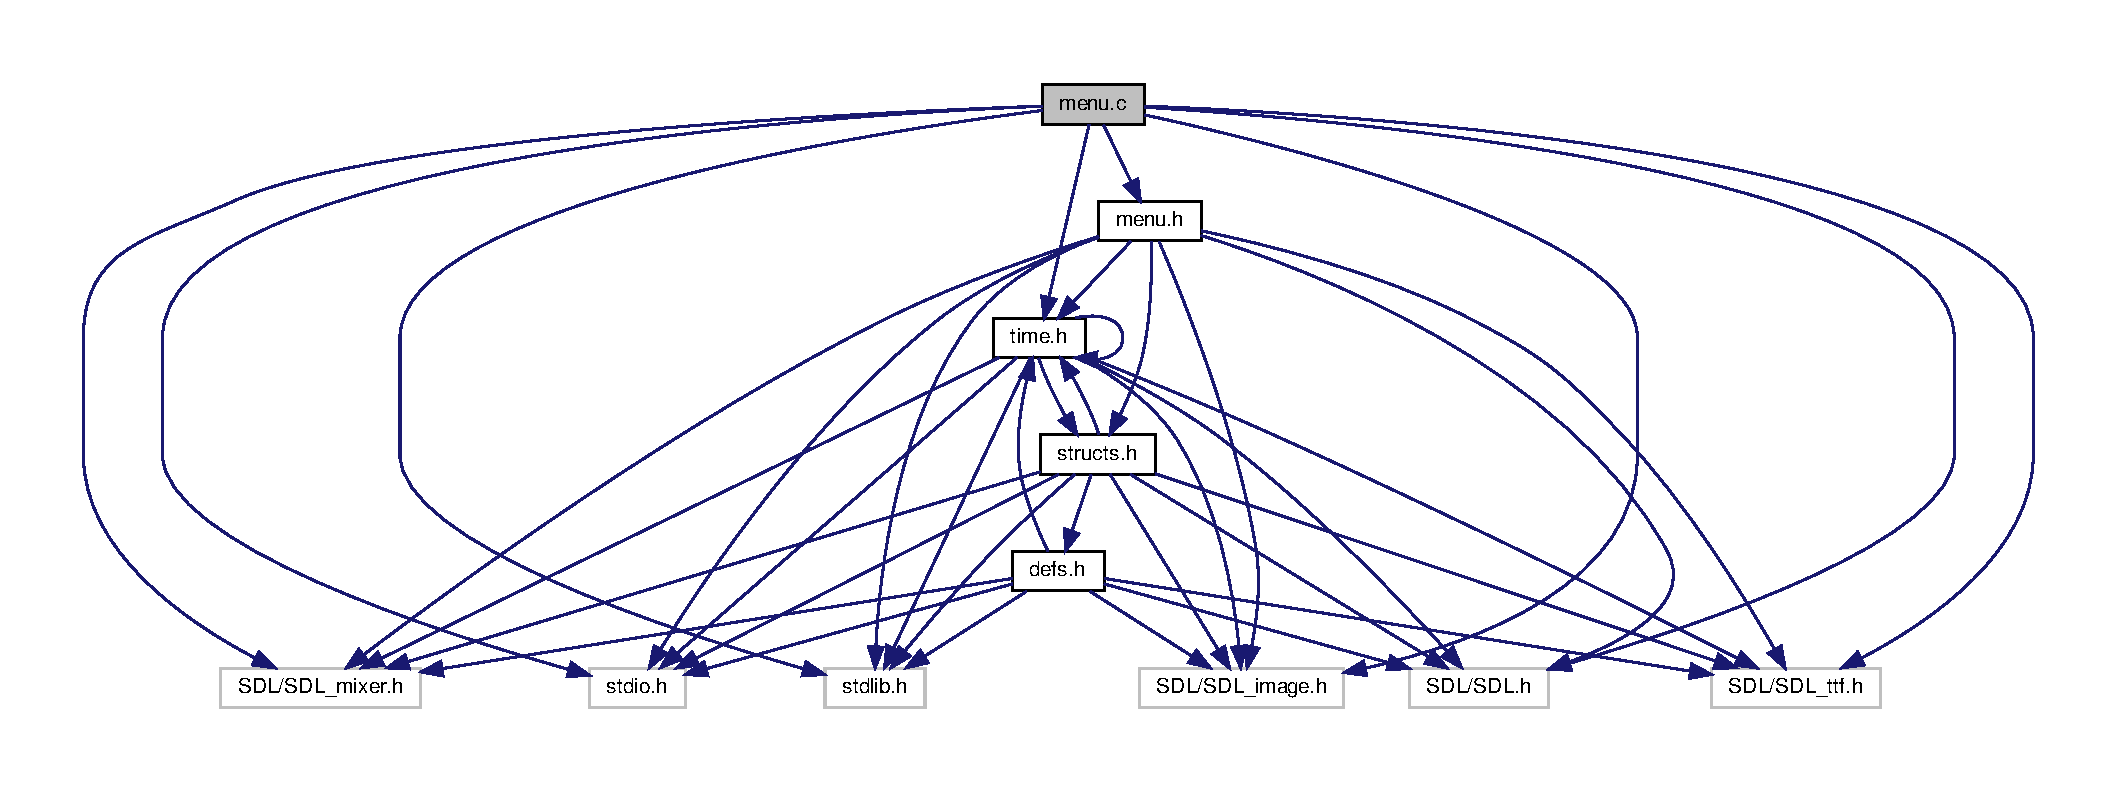
\includegraphics[width=350pt]{menu_8c__incl}
\end{center}
\end{figure}
\subsection*{Functions}
\begin{DoxyCompactItemize}
\item 
\mbox{\Hypertarget{menu_8c_aae463d1e116e9f197e8ef3b57921b9ef}\label{menu_8c_aae463d1e116e9f197e8ef3b57921b9ef}} 
void {\bfseries update\+Start\+Menu} (void)
\item 
\mbox{\Hypertarget{menu_8c_a26264b41bc80c31676cc5e96eec1c1ea}\label{menu_8c_a26264b41bc80c31676cc5e96eec1c1ea}} 
void {\bfseries afficher\+Menu} (void)
\item 
\mbox{\Hypertarget{menu_8c_a21e3832738b06825a629ec3ecaaf1b2b}\label{menu_8c_a21e3832738b06825a629ec3ecaaf1b2b}} 
void {\bfseries affichersettings} (void)
\item 
\mbox{\Hypertarget{menu_8c_af5af767f3a960d64d3b7d8b0b5fafe44}\label{menu_8c_af5af767f3a960d64d3b7d8b0b5fafe44}} 
void {\bfseries update\+Pause\+Menu} (void)
\item 
\mbox{\Hypertarget{menu_8c_a1618af7bc7312d65af6af527c4cc113f}\label{menu_8c_a1618af7bc7312d65af6af527c4cc113f}} 
void {\bfseries afficherpause} (void)
\item 
\mbox{\Hypertarget{menu_8c_a97972c57bf2531c18f2ed559e1b2e7b1}\label{menu_8c_a97972c57bf2531c18f2ed559e1b2e7b1}} 
void {\bfseries affichermenu2} (void)
\item 
\mbox{\Hypertarget{menu_8c_a9c6df7f3612b4b7bd6997c90adac79b6}\label{menu_8c_a9c6df7f3612b4b7bd6997c90adac79b6}} 
void {\bfseries afficherexit} (void)
\end{DoxyCompactItemize}


\subsection{Detailed Description}
menu libs 

\begin{DoxyAuthor}{Author}
Dynamic 
\end{DoxyAuthor}
\begin{DoxyVersion}{Version}
1.\+0 
\end{DoxyVersion}
\begin{DoxyDate}{Date}
07/06/2020 
\end{DoxyDate}

\hypertarget{menu_8h}{}\section{menu.\+h File Reference}
\label{menu_8h}\index{menu.\+h@{menu.\+h}}


menu libs  


{\ttfamily \#include $<$stdlib.\+h$>$}\newline
{\ttfamily \#include $<$stdio.\+h$>$}\newline
{\ttfamily \#include $<$S\+D\+L/\+S\+D\+L.\+h$>$}\newline
{\ttfamily \#include $<$S\+D\+L/\+S\+D\+L\+\_\+image.\+h$>$}\newline
{\ttfamily \#include $<$S\+D\+L/\+S\+D\+L\+\_\+mixer.\+h$>$}\newline
{\ttfamily \#include $<$S\+D\+L/\+S\+D\+L\+\_\+ttf.\+h$>$}\newline
{\ttfamily \#include $<$time.\+h$>$}\newline
{\ttfamily \#include \char`\"{}structs.\+h\char`\"{}}\newline
Include dependency graph for menu.\+h\+:
\nopagebreak
\begin{figure}[H]
\begin{center}
\leavevmode
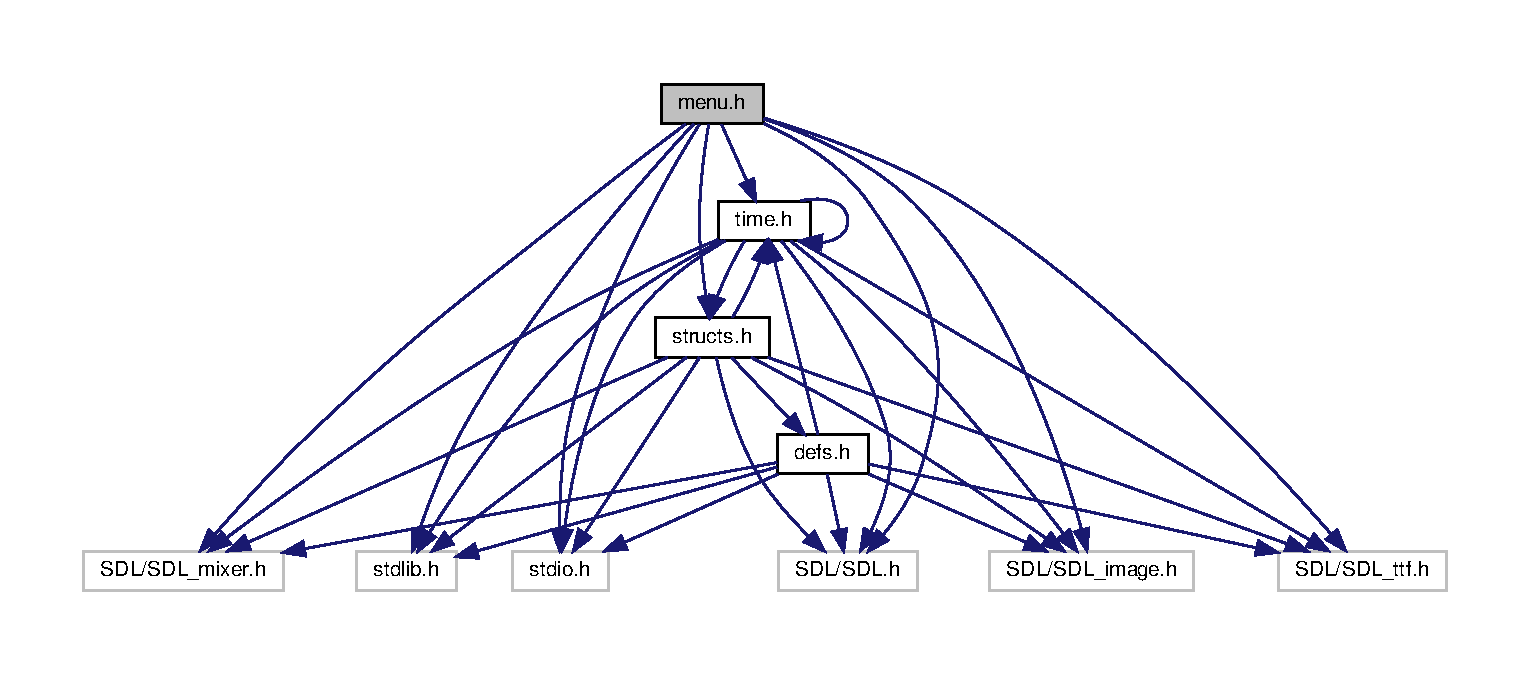
\includegraphics[width=350pt]{menu_8h__incl}
\end{center}
\end{figure}
This graph shows which files directly or indirectly include this file\+:
\nopagebreak
\begin{figure}[H]
\begin{center}
\leavevmode
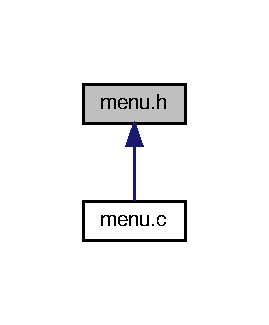
\includegraphics[width=129pt]{menu_8h__dep__incl}
\end{center}
\end{figure}
\subsection*{Functions}
\begin{DoxyCompactItemize}
\item 
\mbox{\Hypertarget{menu_8h_a83d0894aca32e4162ff85241c123286c}\label{menu_8h_a83d0894aca32e4162ff85241c123286c}} 
void {\bfseries draw\+String} (char $\ast$text, int x, int y, T\+T\+F\+\_\+\+Font $\ast$font)
\item 
\mbox{\Hypertarget{menu_8h_a0878703c44d068d3bddfa7f6705affb7}\label{menu_8h_a0878703c44d068d3bddfa7f6705affb7}} 
void {\bfseries change\+Level} (void)
\item 
\mbox{\Hypertarget{menu_8h_a644062856718cc167784b35256ef6132}\label{menu_8h_a644062856718cc167784b35256ef6132}} 
void {\bfseries initialize\+Player} (void)
\item 
\mbox{\Hypertarget{menu_8h_af646d273a1348946bb843f25e39a58bb}\label{menu_8h_af646d273a1348946bb843f25e39a58bb}} 
void {\bfseries draw\+\_\+\+String} (char $\ast$text, int x, int y, T\+T\+F\+\_\+\+Font $\ast$font)
\item 
\mbox{\Hypertarget{menu_8h_adadba7f4b031f83e75a7a3b1c6422e51}\label{menu_8h_adadba7f4b031f83e75a7a3b1c6422e51}} 
void {\bfseries save} (\hyperlink{structHero}{Hero} player, \hyperlink{structGestion}{Gestion} jeu, \hyperlink{structMap}{Map} map, char nom\+Fich\mbox{[}$\,$\mbox{]})
\item 
\mbox{\Hypertarget{menu_8h_a229189c8cd63f8858a396ac7d374202e}\label{menu_8h_a229189c8cd63f8858a396ac7d374202e}} 
void {\bfseries load} (\hyperlink{structHero}{Hero} $\ast$player, \hyperlink{structGestion}{Gestion} $\ast$jeu, \hyperlink{structMap}{Map} $\ast$map, char nom\+Fich\mbox{[}$\,$\mbox{]})
\item 
\mbox{\Hypertarget{menu_8h_af6b3bf14e76f3d6bbda542457e8066a3}\label{menu_8h_af6b3bf14e76f3d6bbda542457e8066a3}} 
void {\bfseries Sound} (int type)
\item 
\mbox{\Hypertarget{menu_8h_aa0cca3ec336bfaa20ec2bfc23c68d126}\label{menu_8h_aa0cca3ec336bfaa20ec2bfc23c68d126}} 
void {\bfseries initialize\+Monster} ()
\item 
\mbox{\Hypertarget{menu_8h_ae79e00c8c17b1a8ba7cf841be6cd0ffd}\label{menu_8h_ae79e00c8c17b1a8ba7cf841be6cd0ffd}} 
void {\bfseries change\+Animation} (\hyperlink{structHero}{Hero} $\ast$entity, char $\ast$name)
\item 
\mbox{\Hypertarget{menu_8h_a12b9f50e1f51a4019b2b5cb8c8ed04b8}\label{menu_8h_a12b9f50e1f51a4019b2b5cb8c8ed04b8}} 
S\+D\+L\+\_\+\+Surface $\ast$ {\bfseries load\+Image} (char $\ast$name)
\end{DoxyCompactItemize}
\subsection*{Variables}
\begin{DoxyCompactItemize}
\item 
\mbox{\Hypertarget{menu_8h_abbeff4ee7b328d6b61b563ecded5bf83}\label{menu_8h_abbeff4ee7b328d6b61b563ecded5bf83}} 
\hyperlink{structGestion}{Gestion} {\bfseries jeu}
\item 
\mbox{\Hypertarget{menu_8h_abf5bfa705e66ffc1ddaa6ce46c960873}\label{menu_8h_abf5bfa705e66ffc1ddaa6ce46c960873}} 
T\+T\+F\+\_\+\+Font $\ast$ {\bfseries font}
\item 
\mbox{\Hypertarget{menu_8h_ad4db59ccea8946af2bb70f8269e99eeb}\label{menu_8h_ad4db59ccea8946af2bb70f8269e99eeb}} 
\hyperlink{structInput}{Input} {\bfseries input}
\item 
\mbox{\Hypertarget{menu_8h_a7a56ddcc26459f1d1b0391d1a2025448}\label{menu_8h_a7a56ddcc26459f1d1b0391d1a2025448}} 
\hyperlink{structHero}{Hero} {\bfseries player}
\item 
\mbox{\Hypertarget{menu_8h_a2737dcd286631af70eac9ebd6de78a07}\label{menu_8h_a2737dcd286631af70eac9ebd6de78a07}} 
\hyperlink{structHero}{Hero} {\bfseries monster}
\item 
\mbox{\Hypertarget{menu_8h_ac9becb8e2f80125547c8cc8f9d56b7ab}\label{menu_8h_ac9becb8e2f80125547c8cc8f9d56b7ab}} 
\hyperlink{structMap}{Map} {\bfseries map}
\item 
\mbox{\Hypertarget{menu_8h_a32175bc9c482ed465d43f3e1d31f72a4}\label{menu_8h_a32175bc9c482ed465d43f3e1d31f72a4}} 
\hyperlink{structGameobject}{Gameobject} {\bfseries star}
\end{DoxyCompactItemize}


\subsection{Detailed Description}
menu libs 

\begin{DoxyAuthor}{Author}
Dynamic 
\end{DoxyAuthor}
\begin{DoxyVersion}{Version}
1.\+0 
\end{DoxyVersion}
\begin{DoxyDate}{Date}
07/06/2020 
\end{DoxyDate}

\hypertarget{minimap_8c}{}\section{minimap.\+c File Reference}
\label{minimap_8c}\index{minimap.\+c@{minimap.\+c}}


minimap libs  


{\ttfamily \#include $<$stdlib.\+h$>$}\newline
{\ttfamily \#include $<$stdio.\+h$>$}\newline
{\ttfamily \#include $<$S\+D\+L/\+S\+D\+L.\+h$>$}\newline
{\ttfamily \#include $<$S\+D\+L/\+S\+D\+L\+\_\+image.\+h$>$}\newline
{\ttfamily \#include $<$S\+D\+L/\+S\+D\+L\+\_\+mixer.\+h$>$}\newline
{\ttfamily \#include $<$S\+D\+L/\+S\+D\+L\+\_\+ttf.\+h$>$}\newline
{\ttfamily \#include $<$time.\+h$>$}\newline
{\ttfamily \#include $<$string.\+h$>$}\newline
{\ttfamily \#include $<$unistd.\+h$>$}\newline
{\ttfamily \#include \char`\"{}minimap.\+h\char`\"{}}\newline
Include dependency graph for minimap.\+c\+:
\nopagebreak
\begin{figure}[H]
\begin{center}
\leavevmode
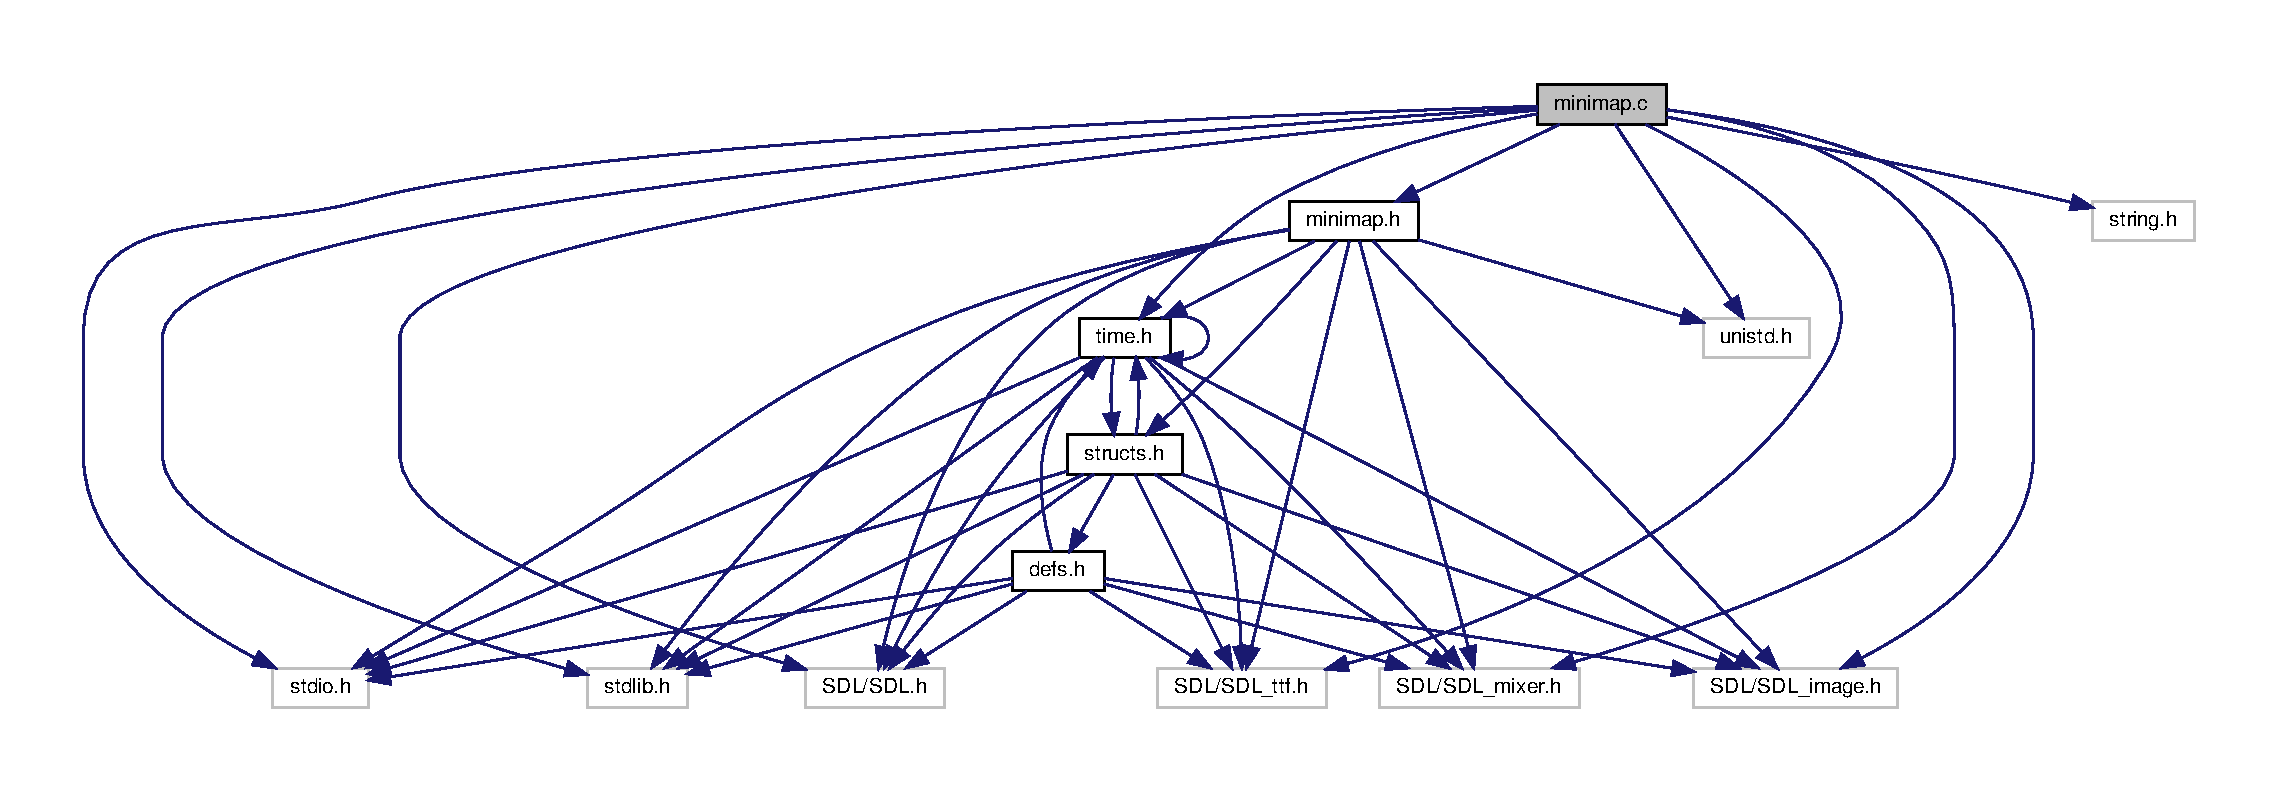
\includegraphics[width=350pt]{minimap_8c__incl}
\end{center}
\end{figure}
\subsection*{Functions}
\begin{DoxyCompactItemize}
\item 
\mbox{\Hypertarget{minimap_8c_ac1dd451bf94ab9d190866bf42aad3dbd}\label{minimap_8c_ac1dd451bf94ab9d190866bf42aad3dbd}} 
void {\bfseries Afficher\+\_\+\+Minimap} (S\+D\+L\+\_\+\+Surface $\ast$screen, S\+D\+L\+\_\+\+Rect posplayer, S\+D\+L\+\_\+\+Rect posmonster, S\+D\+L\+\_\+\+Rect posstar)
\item 
\mbox{\Hypertarget{minimap_8c_a71b27710c1dad331f8c84e5a9be05f1c}\label{minimap_8c_a71b27710c1dad331f8c84e5a9be05f1c}} 
S\+D\+L\+\_\+\+Rect {\bfseries make\+It\+Small} (S\+D\+L\+\_\+\+Rect minimap, S\+D\+L\+\_\+\+Rect position)
\end{DoxyCompactItemize}


\subsection{Detailed Description}
minimap libs 

\begin{DoxyAuthor}{Author}
Raed 
\end{DoxyAuthor}
\begin{DoxyVersion}{Version}
1.\+0 
\end{DoxyVersion}
\begin{DoxyDate}{Date}
07/06/2020 
\end{DoxyDate}

\hypertarget{minimap_8h}{}\section{minimap.\+h File Reference}
\label{minimap_8h}\index{minimap.\+h@{minimap.\+h}}


minimap libs  


{\ttfamily \#include $<$stdlib.\+h$>$}\newline
{\ttfamily \#include $<$stdio.\+h$>$}\newline
{\ttfamily \#include $<$S\+D\+L/\+S\+D\+L.\+h$>$}\newline
{\ttfamily \#include $<$S\+D\+L/\+S\+D\+L\+\_\+image.\+h$>$}\newline
{\ttfamily \#include $<$S\+D\+L/\+S\+D\+L\+\_\+mixer.\+h$>$}\newline
{\ttfamily \#include $<$S\+D\+L/\+S\+D\+L\+\_\+ttf.\+h$>$}\newline
{\ttfamily \#include $<$time.\+h$>$}\newline
{\ttfamily \#include $<$unistd.\+h$>$}\newline
{\ttfamily \#include \char`\"{}structs.\+h\char`\"{}}\newline
Include dependency graph for minimap.\+h\+:
\nopagebreak
\begin{figure}[H]
\begin{center}
\leavevmode
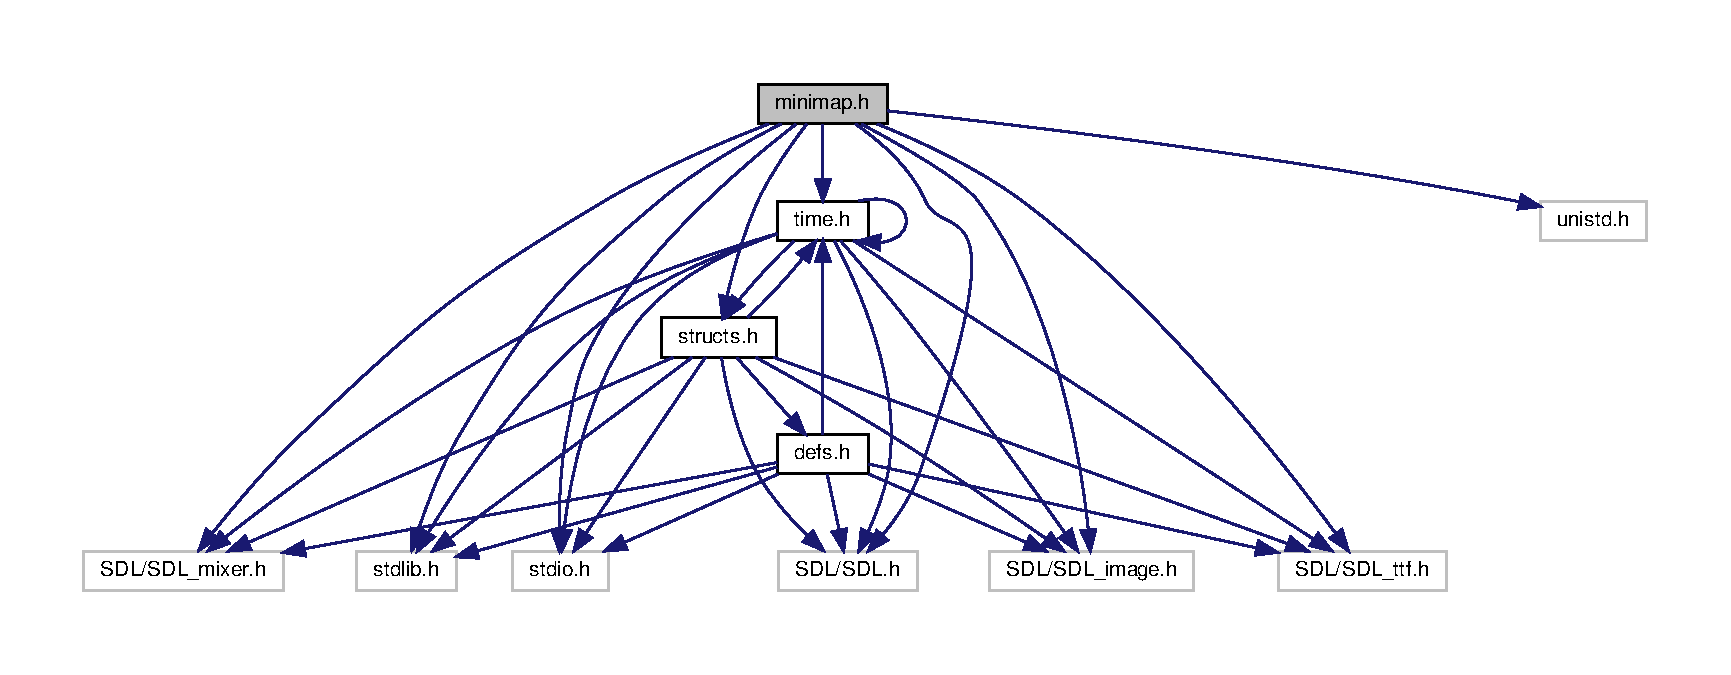
\includegraphics[width=350pt]{minimap_8h__incl}
\end{center}
\end{figure}
This graph shows which files directly or indirectly include this file\+:
\nopagebreak
\begin{figure}[H]
\begin{center}
\leavevmode
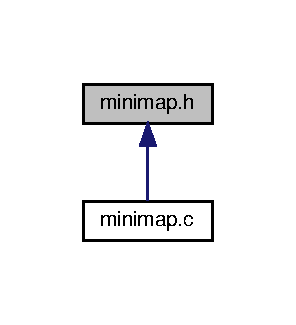
\includegraphics[width=142pt]{minimap_8h__dep__incl}
\end{center}
\end{figure}
\subsection*{Functions}
\begin{DoxyCompactItemize}
\item 
\mbox{\Hypertarget{minimap_8h_ac1dd451bf94ab9d190866bf42aad3dbd}\label{minimap_8h_ac1dd451bf94ab9d190866bf42aad3dbd}} 
void {\bfseries Afficher\+\_\+\+Minimap} (S\+D\+L\+\_\+\+Surface $\ast$screen, S\+D\+L\+\_\+\+Rect posplayer, S\+D\+L\+\_\+\+Rect posmonster, S\+D\+L\+\_\+\+Rect posstar)
\item 
\mbox{\Hypertarget{minimap_8h_a71b27710c1dad331f8c84e5a9be05f1c}\label{minimap_8h_a71b27710c1dad331f8c84e5a9be05f1c}} 
S\+D\+L\+\_\+\+Rect {\bfseries make\+It\+Small} (S\+D\+L\+\_\+\+Rect minimap, S\+D\+L\+\_\+\+Rect position)
\end{DoxyCompactItemize}
\subsection*{Variables}
\begin{DoxyCompactItemize}
\item 
\mbox{\Hypertarget{minimap_8h_abbeff4ee7b328d6b61b563ecded5bf83}\label{minimap_8h_abbeff4ee7b328d6b61b563ecded5bf83}} 
\hyperlink{structGestion}{Gestion} {\bfseries jeu}
\item 
\mbox{\Hypertarget{minimap_8h_ac9becb8e2f80125547c8cc8f9d56b7ab}\label{minimap_8h_ac9becb8e2f80125547c8cc8f9d56b7ab}} 
\hyperlink{structMap}{Map} {\bfseries map}
\item 
\mbox{\Hypertarget{minimap_8h_a7a56ddcc26459f1d1b0391d1a2025448}\label{minimap_8h_a7a56ddcc26459f1d1b0391d1a2025448}} 
\hyperlink{structHero}{Hero} {\bfseries player}
\item 
\mbox{\Hypertarget{minimap_8h_a2737dcd286631af70eac9ebd6de78a07}\label{minimap_8h_a2737dcd286631af70eac9ebd6de78a07}} 
\hyperlink{structHero}{Hero} {\bfseries monster}
\item 
\mbox{\Hypertarget{minimap_8h_a32175bc9c482ed465d43f3e1d31f72a4}\label{minimap_8h_a32175bc9c482ed465d43f3e1d31f72a4}} 
\hyperlink{structGameobject}{Gameobject} {\bfseries star}
\end{DoxyCompactItemize}


\subsection{Detailed Description}
minimap libs 

\begin{DoxyAuthor}{Author}
Raed 
\end{DoxyAuthor}
\begin{DoxyVersion}{Version}
1.\+0 
\end{DoxyVersion}
\begin{DoxyDate}{Date}
07/06/2020 
\end{DoxyDate}

\hypertarget{monster_8c}{}\section{monster.\+c File Reference}
\label{monster_8c}\index{monster.\+c@{monster.\+c}}


monster libs  


{\ttfamily \#include $<$stdlib.\+h$>$}\newline
{\ttfamily \#include $<$stdio.\+h$>$}\newline
{\ttfamily \#include $<$S\+D\+L/\+S\+D\+L.\+h$>$}\newline
{\ttfamily \#include $<$S\+D\+L/\+S\+D\+L\+\_\+image.\+h$>$}\newline
{\ttfamily \#include $<$S\+D\+L/\+S\+D\+L\+\_\+mixer.\+h$>$}\newline
{\ttfamily \#include $<$S\+D\+L/\+S\+D\+L\+\_\+ttf.\+h$>$}\newline
{\ttfamily \#include $<$time.\+h$>$}\newline
{\ttfamily \#include \char`\"{}monster.\+h\char`\"{}}\newline
Include dependency graph for monster.\+c\+:
\nopagebreak
\begin{figure}[H]
\begin{center}
\leavevmode
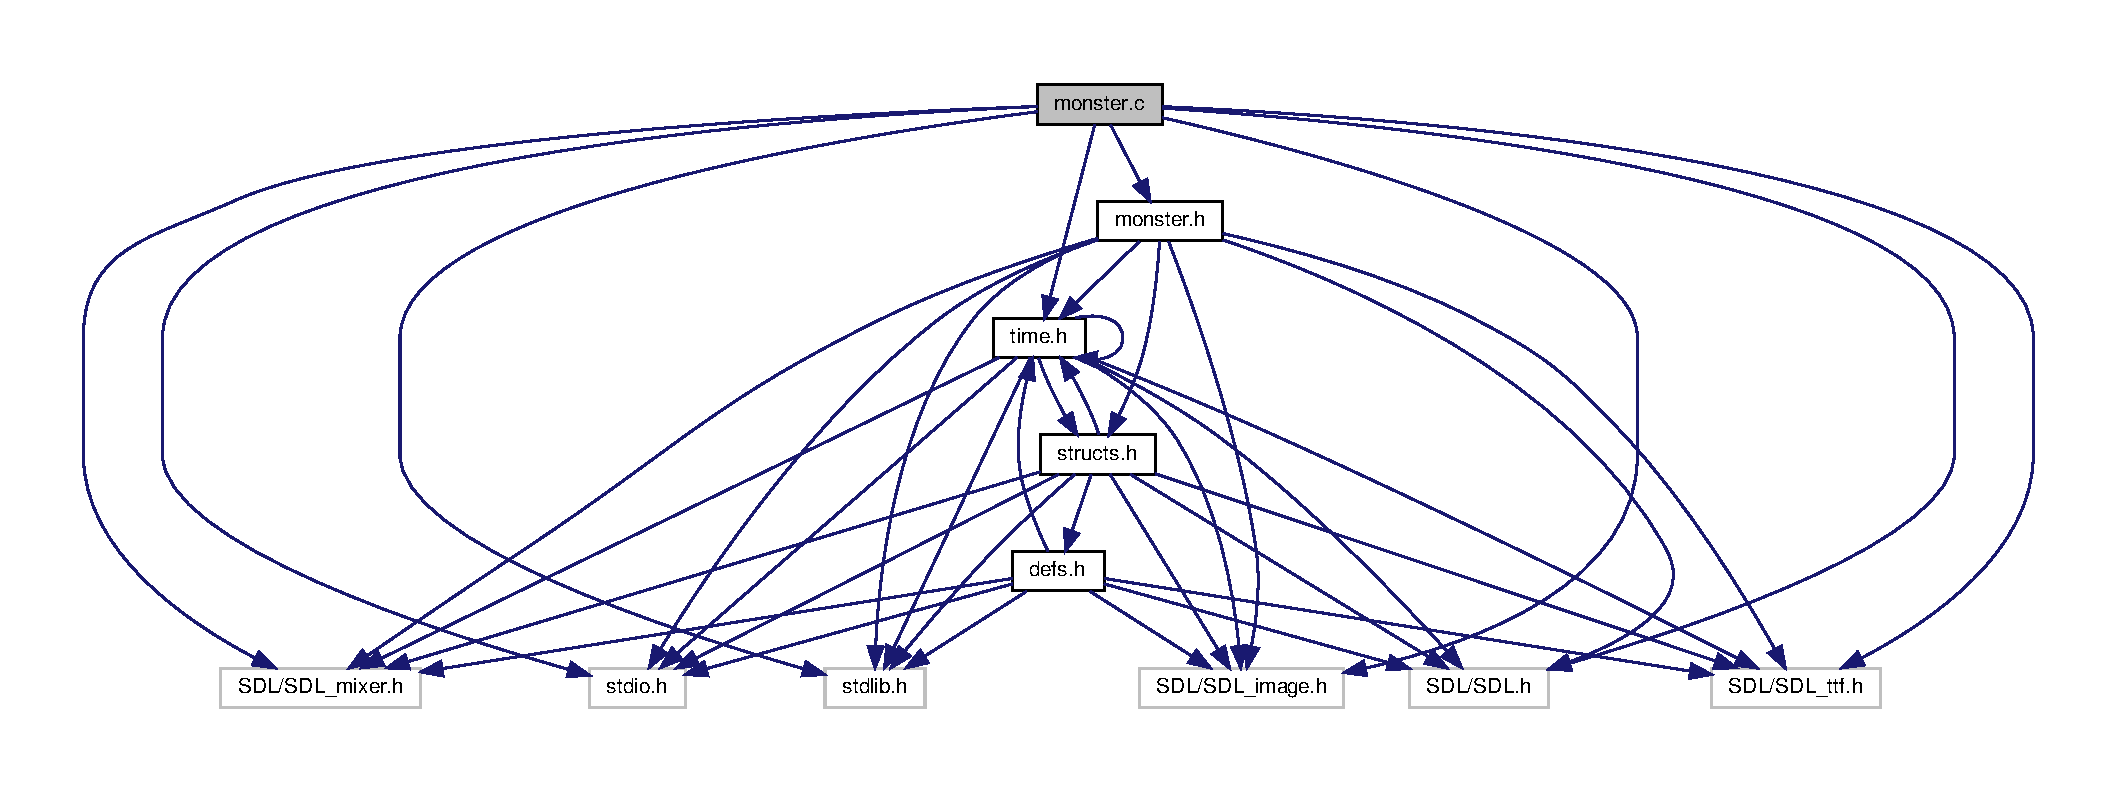
\includegraphics[width=350pt]{monster_8c__incl}
\end{center}
\end{figure}
\subsection*{Functions}
\begin{DoxyCompactItemize}
\item 
\mbox{\Hypertarget{monster_8c_a1ef3f5345244e012b588b9865263afcd}\label{monster_8c_a1ef3f5345244e012b588b9865263afcd}} 
void {\bfseries initialize\+Monster} (void)
\item 
\mbox{\Hypertarget{monster_8c_a9f6a40109157219079a70db323cf777a}\label{monster_8c_a9f6a40109157219079a70db323cf777a}} 
void {\bfseries afficher\+Monster} ()
\item 
\mbox{\Hypertarget{monster_8c_a2adf3d6df9899ef24364a58289874ec9}\label{monster_8c_a2adf3d6df9899ef24364a58289874ec9}} 
void {\bfseries update\+Monster} (void)
\end{DoxyCompactItemize}


\subsection{Detailed Description}
monster libs 

\begin{DoxyAuthor}{Author}
skander+cyrine 
\end{DoxyAuthor}
\begin{DoxyVersion}{Version}
1.\+0 
\end{DoxyVersion}
\begin{DoxyDate}{Date}
07/06/2020 
\end{DoxyDate}

\hypertarget{monster_8h}{}\section{monster.\+h File Reference}
\label{monster_8h}\index{monster.\+h@{monster.\+h}}


monster libs  


{\ttfamily \#include $<$stdlib.\+h$>$}\newline
{\ttfamily \#include $<$stdio.\+h$>$}\newline
{\ttfamily \#include $<$S\+D\+L/\+S\+D\+L.\+h$>$}\newline
{\ttfamily \#include $<$S\+D\+L/\+S\+D\+L\+\_\+image.\+h$>$}\newline
{\ttfamily \#include $<$S\+D\+L/\+S\+D\+L\+\_\+mixer.\+h$>$}\newline
{\ttfamily \#include $<$S\+D\+L/\+S\+D\+L\+\_\+ttf.\+h$>$}\newline
{\ttfamily \#include $<$time.\+h$>$}\newline
{\ttfamily \#include \char`\"{}structs.\+h\char`\"{}}\newline
Include dependency graph for monster.\+h\+:
\nopagebreak
\begin{figure}[H]
\begin{center}
\leavevmode
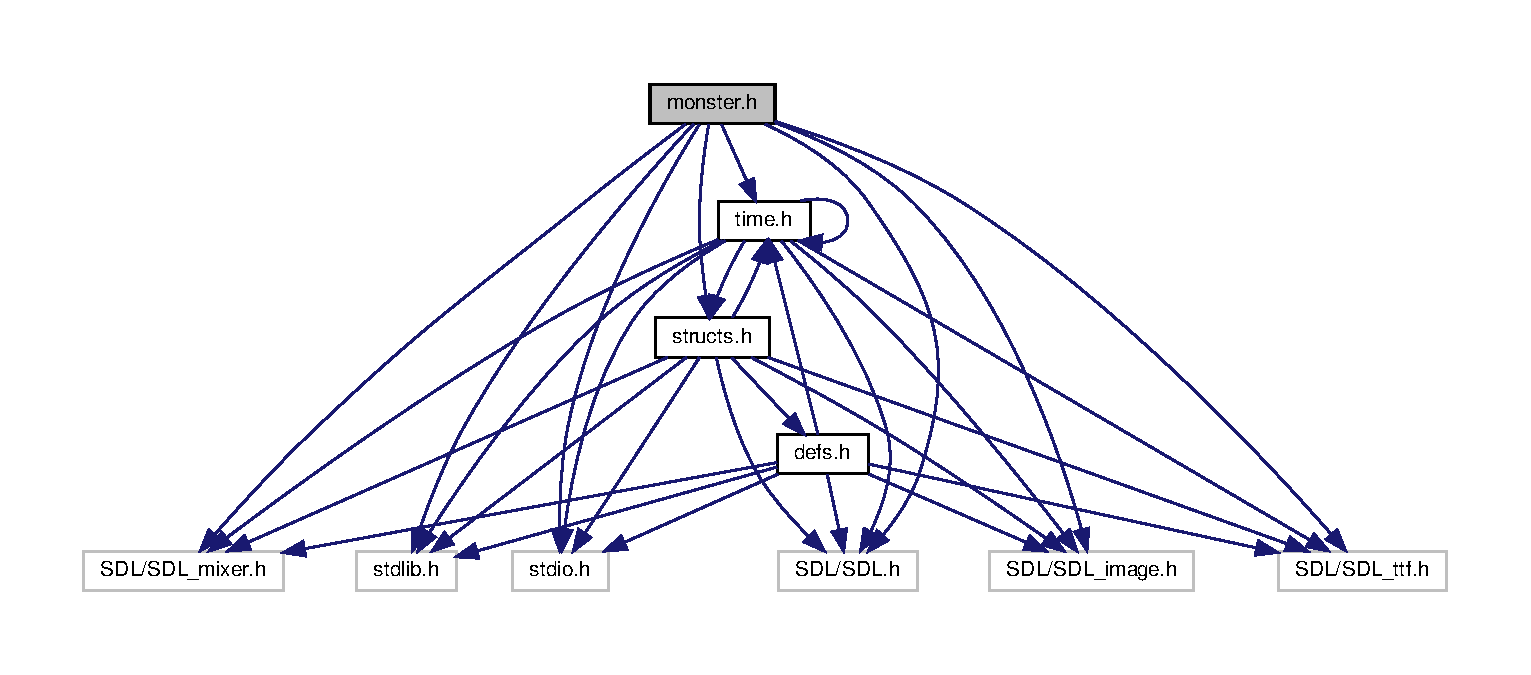
\includegraphics[width=350pt]{monster_8h__incl}
\end{center}
\end{figure}
This graph shows which files directly or indirectly include this file\+:
\nopagebreak
\begin{figure}[H]
\begin{center}
\leavevmode
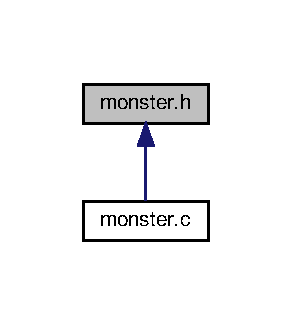
\includegraphics[width=140pt]{monster_8h__dep__incl}
\end{center}
\end{figure}
\subsection*{Functions}
\begin{DoxyCompactItemize}
\item 
\mbox{\Hypertarget{monster_8h_a12b9f50e1f51a4019b2b5cb8c8ed04b8}\label{monster_8h_a12b9f50e1f51a4019b2b5cb8c8ed04b8}} 
S\+D\+L\+\_\+\+Surface $\ast$ {\bfseries load\+Image} (char $\ast$name)
\item 
\mbox{\Hypertarget{monster_8h_af6b3bf14e76f3d6bbda542457e8066a3}\label{monster_8h_af6b3bf14e76f3d6bbda542457e8066a3}} 
void {\bfseries Sound} (int type)
\item 
\mbox{\Hypertarget{monster_8h_ae79e00c8c17b1a8ba7cf841be6cd0ffd}\label{monster_8h_ae79e00c8c17b1a8ba7cf841be6cd0ffd}} 
void {\bfseries change\+Animation} (\hyperlink{structHero}{Hero} $\ast$entity, char $\ast$name)
\end{DoxyCompactItemize}
\subsection*{Variables}
\begin{DoxyCompactItemize}
\item 
\mbox{\Hypertarget{monster_8h_abbeff4ee7b328d6b61b563ecded5bf83}\label{monster_8h_abbeff4ee7b328d6b61b563ecded5bf83}} 
\hyperlink{structGestion}{Gestion} {\bfseries jeu}
\item 
\mbox{\Hypertarget{monster_8h_a2737dcd286631af70eac9ebd6de78a07}\label{monster_8h_a2737dcd286631af70eac9ebd6de78a07}} 
\hyperlink{structHero}{Hero} {\bfseries monster}
\item 
\mbox{\Hypertarget{monster_8h_ad4db59ccea8946af2bb70f8269e99eeb}\label{monster_8h_ad4db59ccea8946af2bb70f8269e99eeb}} 
\hyperlink{structInput}{Input} {\bfseries input}
\item 
\mbox{\Hypertarget{monster_8h_ac9becb8e2f80125547c8cc8f9d56b7ab}\label{monster_8h_ac9becb8e2f80125547c8cc8f9d56b7ab}} 
\hyperlink{structMap}{Map} {\bfseries map}
\item 
\mbox{\Hypertarget{monster_8h_a46bbb8f0ca78423455fee2bbf4549165}\label{monster_8h_a46bbb8f0ca78423455fee2bbf4549165}} 
\hyperlink{structGameobject}{Gameobject} {\bfseries objet}
\end{DoxyCompactItemize}


\subsection{Detailed Description}
monster libs 

\begin{DoxyAuthor}{Author}
skander+cyrine 
\end{DoxyAuthor}
\begin{DoxyVersion}{Version}
1.\+0 
\end{DoxyVersion}
\begin{DoxyDate}{Date}
07/06/2020 
\end{DoxyDate}

\hypertarget{musique_8c}{}\section{musique.\+c File Reference}
\label{musique_8c}\index{musique.\+c@{musique.\+c}}


musique libs  


{\ttfamily \#include $<$stdlib.\+h$>$}\newline
{\ttfamily \#include $<$stdio.\+h$>$}\newline
{\ttfamily \#include $<$S\+D\+L/\+S\+D\+L.\+h$>$}\newline
{\ttfamily \#include $<$S\+D\+L/\+S\+D\+L\+\_\+image.\+h$>$}\newline
{\ttfamily \#include $<$S\+D\+L/\+S\+D\+L\+\_\+mixer.\+h$>$}\newline
{\ttfamily \#include $<$S\+D\+L/\+S\+D\+L\+\_\+ttf.\+h$>$}\newline
{\ttfamily \#include $<$time.\+h$>$}\newline
{\ttfamily \#include \char`\"{}musique.\+h\char`\"{}}\newline
Include dependency graph for musique.\+c\+:
\nopagebreak
\begin{figure}[H]
\begin{center}
\leavevmode
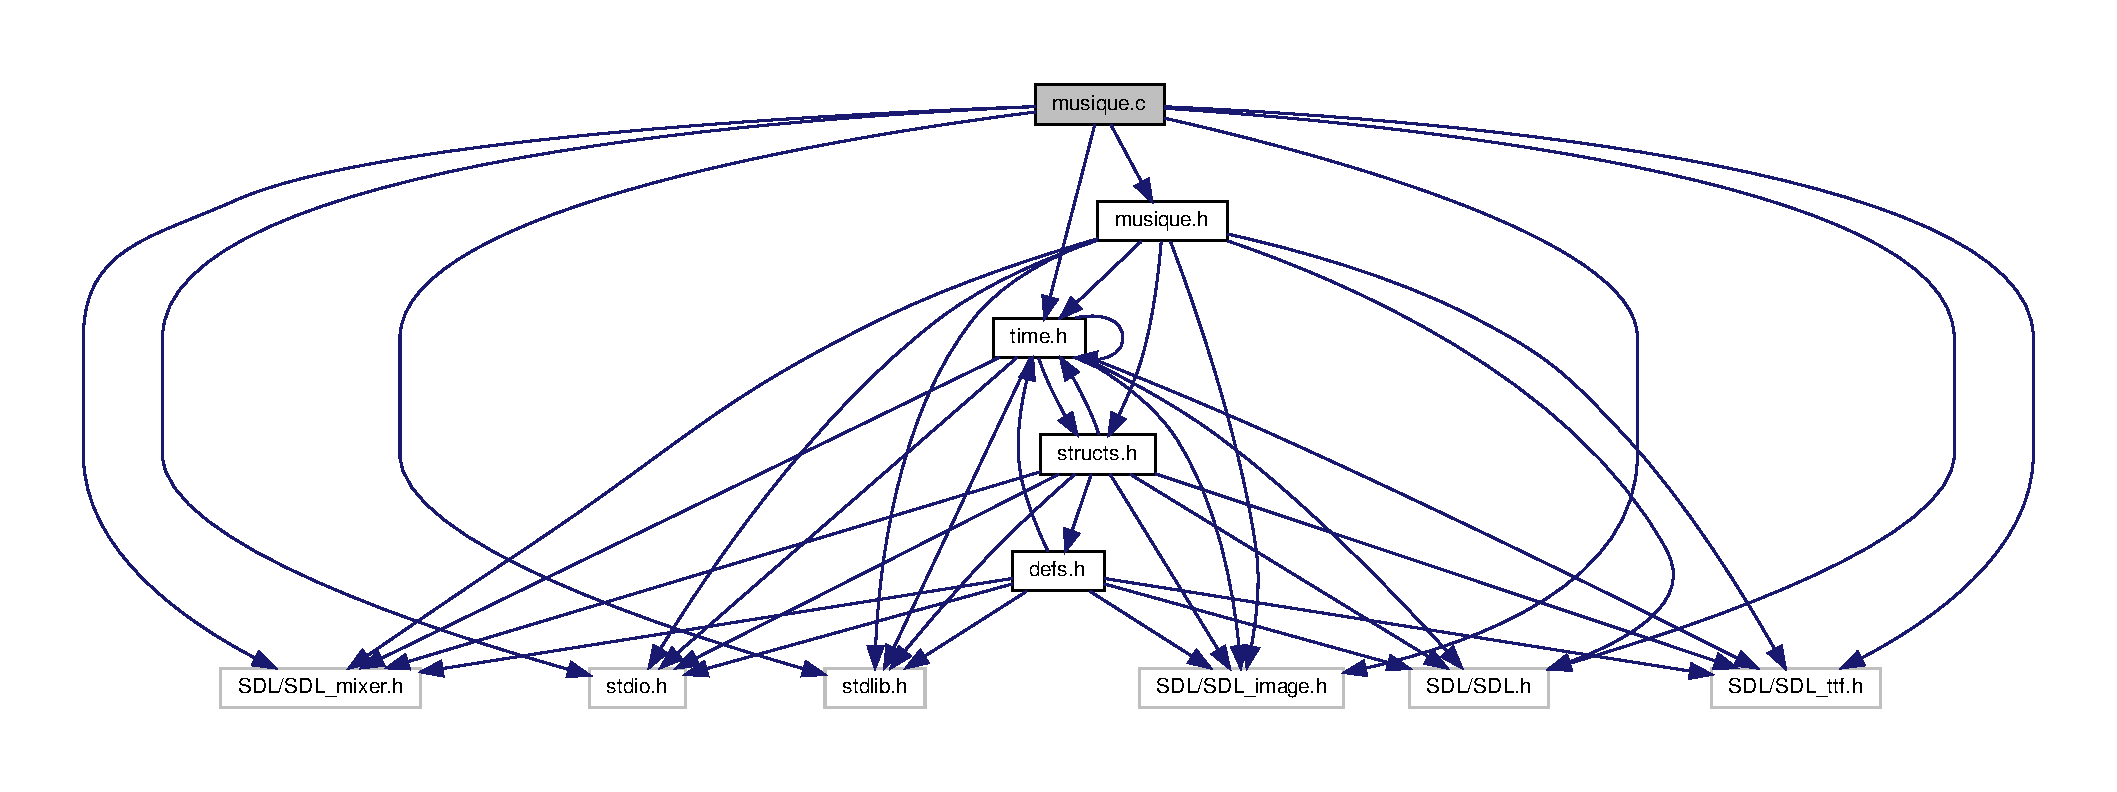
\includegraphics[width=350pt]{musique_8c__incl}
\end{center}
\end{figure}
\subsection*{Functions}
\begin{DoxyCompactItemize}
\item 
\mbox{\Hypertarget{musique_8c_a1c001a82cba133dd3beb5ff6a014a537}\label{musique_8c_a1c001a82cba133dd3beb5ff6a014a537}} 
void {\bfseries load\+Song} (char filename\mbox{[}200\mbox{]})
\item 
\mbox{\Hypertarget{musique_8c_a86eb94e3b6f2b5b7c798dc02b0935500}\label{musique_8c_a86eb94e3b6f2b5b7c798dc02b0935500}} 
void {\bfseries load\+Sound} (void)
\item 
\mbox{\Hypertarget{musique_8c_afed923638f1c2eebd978b79bf62c5919}\label{musique_8c_afed923638f1c2eebd978b79bf62c5919}} 
void {\bfseries free\+Sound} (void)
\item 
\mbox{\Hypertarget{musique_8c_af6b3bf14e76f3d6bbda542457e8066a3}\label{musique_8c_af6b3bf14e76f3d6bbda542457e8066a3}} 
void {\bfseries Sound} (int type)
\end{DoxyCompactItemize}


\subsection{Detailed Description}
musique libs 

\begin{DoxyAuthor}{Author}
Youssef 
\end{DoxyAuthor}
\begin{DoxyVersion}{Version}
1.\+0 
\end{DoxyVersion}
\begin{DoxyDate}{Date}
07/06/2020 
\end{DoxyDate}

\hypertarget{musique_8h}{}\section{musique.\+h File Reference}
\label{musique_8h}\index{musique.\+h@{musique.\+h}}


musique libs  


{\ttfamily \#include $<$stdlib.\+h$>$}\newline
{\ttfamily \#include $<$stdio.\+h$>$}\newline
{\ttfamily \#include $<$S\+D\+L/\+S\+D\+L.\+h$>$}\newline
{\ttfamily \#include $<$S\+D\+L/\+S\+D\+L\+\_\+image.\+h$>$}\newline
{\ttfamily \#include $<$S\+D\+L/\+S\+D\+L\+\_\+mixer.\+h$>$}\newline
{\ttfamily \#include $<$S\+D\+L/\+S\+D\+L\+\_\+ttf.\+h$>$}\newline
{\ttfamily \#include $<$time.\+h$>$}\newline
{\ttfamily \#include \char`\"{}structs.\+h\char`\"{}}\newline
Include dependency graph for musique.\+h\+:
\nopagebreak
\begin{figure}[H]
\begin{center}
\leavevmode
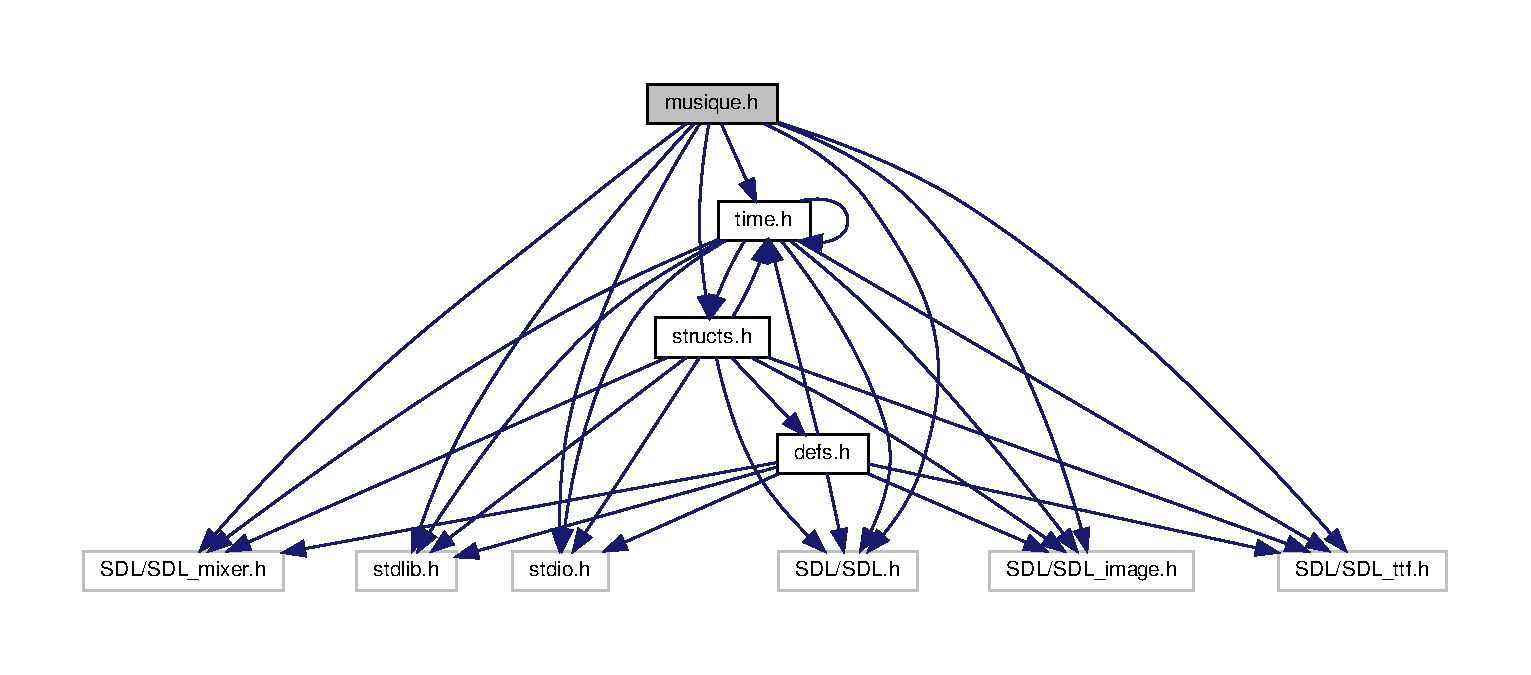
\includegraphics[width=350pt]{musique_8h__incl}
\end{center}
\end{figure}
This graph shows which files directly or indirectly include this file\+:
\nopagebreak
\begin{figure}[H]
\begin{center}
\leavevmode
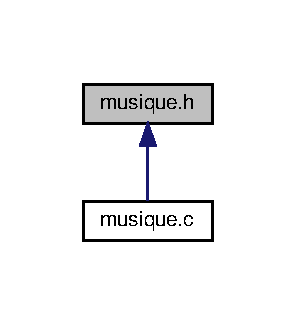
\includegraphics[width=142pt]{musique_8h__dep__incl}
\end{center}
\end{figure}
\subsection*{Variables}
\begin{DoxyCompactItemize}
\item 
\mbox{\Hypertarget{musique_8h_abbeff4ee7b328d6b61b563ecded5bf83}\label{musique_8h_abbeff4ee7b328d6b61b563ecded5bf83}} 
\hyperlink{structGestion}{Gestion} {\bfseries jeu}
\end{DoxyCompactItemize}


\subsection{Detailed Description}
musique libs 

\begin{DoxyAuthor}{Author}
Youssef 
\end{DoxyAuthor}
\begin{DoxyVersion}{Version}
1.\+0 
\end{DoxyVersion}
\begin{DoxyDate}{Date}
07/06/2020 
\end{DoxyDate}

\hypertarget{player_8c}{}\section{player.\+c File Reference}
\label{player_8c}\index{player.\+c@{player.\+c}}


player libs  


{\ttfamily \#include $<$stdlib.\+h$>$}\newline
{\ttfamily \#include $<$stdio.\+h$>$}\newline
{\ttfamily \#include $<$S\+D\+L/\+S\+D\+L.\+h$>$}\newline
{\ttfamily \#include $<$S\+D\+L/\+S\+D\+L\+\_\+image.\+h$>$}\newline
{\ttfamily \#include $<$S\+D\+L/\+S\+D\+L\+\_\+mixer.\+h$>$}\newline
{\ttfamily \#include $<$S\+D\+L/\+S\+D\+L\+\_\+ttf.\+h$>$}\newline
{\ttfamily \#include $<$time.\+h$>$}\newline
{\ttfamily \#include \char`\"{}player.\+h\char`\"{}}\newline
Include dependency graph for player.\+c\+:
\nopagebreak
\begin{figure}[H]
\begin{center}
\leavevmode
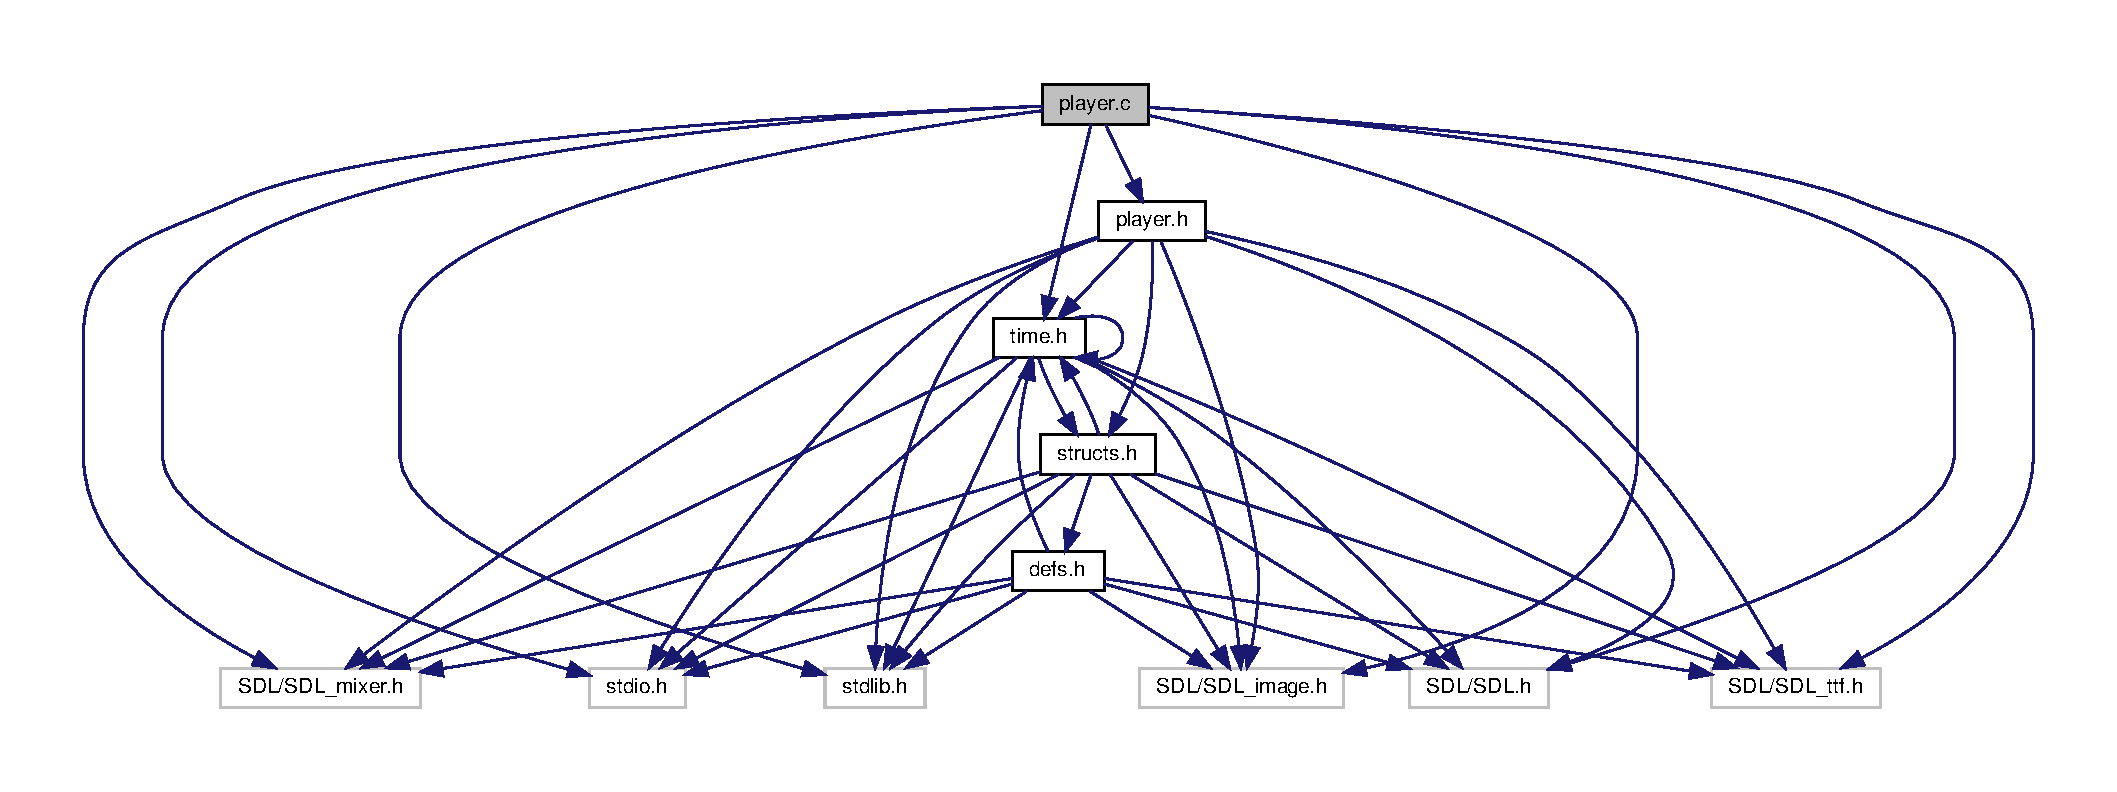
\includegraphics[width=350pt]{player_8c__incl}
\end{center}
\end{figure}
\subsection*{Functions}
\begin{DoxyCompactItemize}
\item 
\mbox{\Hypertarget{player_8c_a644062856718cc167784b35256ef6132}\label{player_8c_a644062856718cc167784b35256ef6132}} 
void {\bfseries initialize\+Player} (void)
\item 
\mbox{\Hypertarget{player_8c_a25c91551bdff9d6ce45d350ce93ab62c}\label{player_8c_a25c91551bdff9d6ce45d350ce93ab62c}} 
void {\bfseries afficherplayer} ()
\item 
\mbox{\Hypertarget{player_8c_a9e55dbb80a29480351146c3dbb1fa6b2}\label{player_8c_a9e55dbb80a29480351146c3dbb1fa6b2}} 
void {\bfseries update\+Player} ()
\end{DoxyCompactItemize}


\subsection{Detailed Description}
player libs 

\begin{DoxyAuthor}{Author}
Yasmine+\+Cyrine 
\end{DoxyAuthor}
\begin{DoxyVersion}{Version}
1.\+0 
\end{DoxyVersion}
\begin{DoxyDate}{Date}
07/06/2020 
\end{DoxyDate}

\hypertarget{player_8h}{}\section{player.\+h File Reference}
\label{player_8h}\index{player.\+h@{player.\+h}}


player libs  


{\ttfamily \#include $<$stdlib.\+h$>$}\newline
{\ttfamily \#include $<$stdio.\+h$>$}\newline
{\ttfamily \#include $<$S\+D\+L/\+S\+D\+L.\+h$>$}\newline
{\ttfamily \#include $<$S\+D\+L/\+S\+D\+L\+\_\+image.\+h$>$}\newline
{\ttfamily \#include $<$S\+D\+L/\+S\+D\+L\+\_\+mixer.\+h$>$}\newline
{\ttfamily \#include $<$S\+D\+L/\+S\+D\+L\+\_\+ttf.\+h$>$}\newline
{\ttfamily \#include $<$time.\+h$>$}\newline
{\ttfamily \#include \char`\"{}structs.\+h\char`\"{}}\newline
Include dependency graph for player.\+h\+:
\nopagebreak
\begin{figure}[H]
\begin{center}
\leavevmode
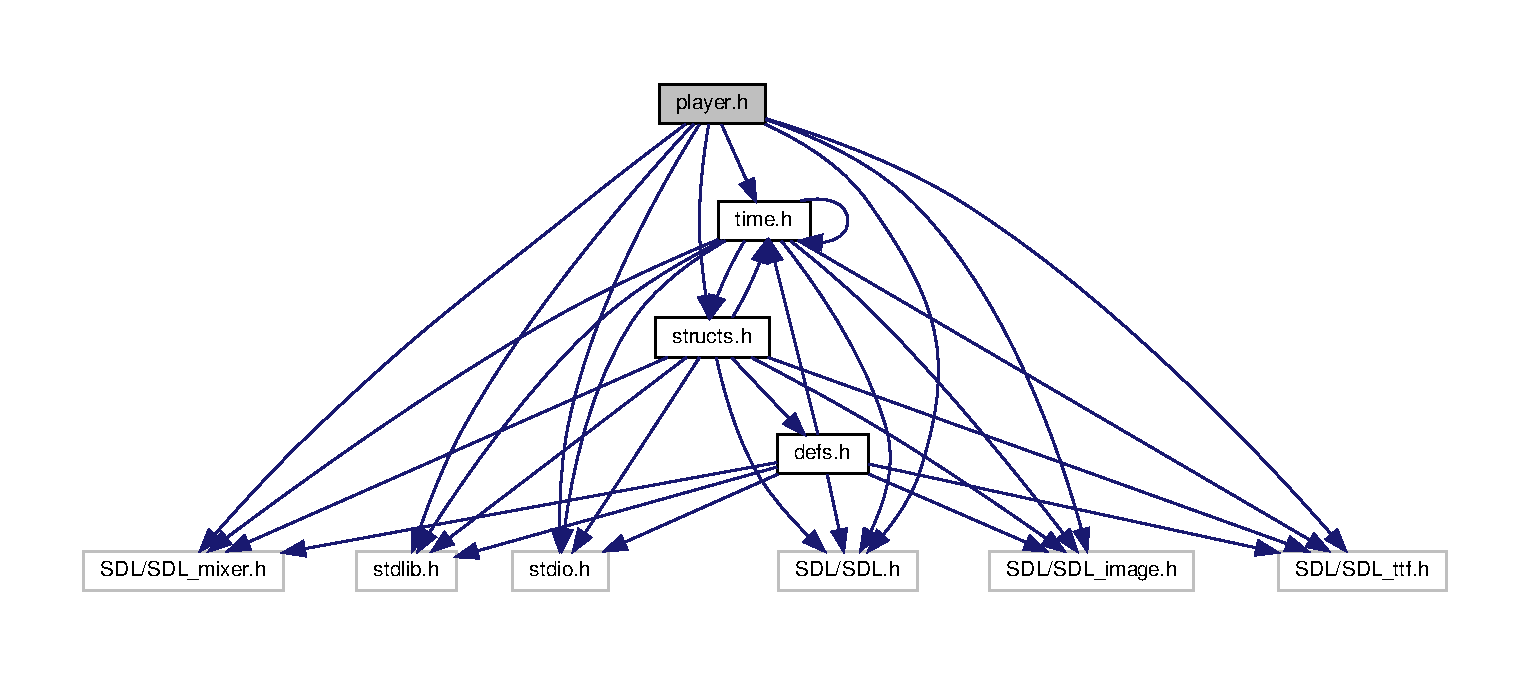
\includegraphics[width=350pt]{player_8h__incl}
\end{center}
\end{figure}
This graph shows which files directly or indirectly include this file\+:
\nopagebreak
\begin{figure}[H]
\begin{center}
\leavevmode
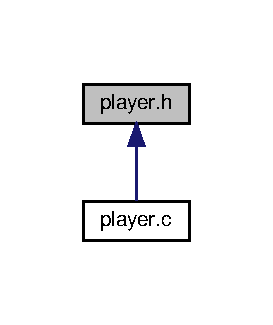
\includegraphics[width=131pt]{player_8h__dep__incl}
\end{center}
\end{figure}
\subsection*{Functions}
\begin{DoxyCompactItemize}
\item 
\mbox{\Hypertarget{player_8h_a12b9f50e1f51a4019b2b5cb8c8ed04b8}\label{player_8h_a12b9f50e1f51a4019b2b5cb8c8ed04b8}} 
S\+D\+L\+\_\+\+Surface $\ast$ {\bfseries load\+Image} (char $\ast$name)
\item 
\mbox{\Hypertarget{player_8h_af6b3bf14e76f3d6bbda542457e8066a3}\label{player_8h_af6b3bf14e76f3d6bbda542457e8066a3}} 
void {\bfseries Sound} (int type)
\item 
\mbox{\Hypertarget{player_8h_ae79e00c8c17b1a8ba7cf841be6cd0ffd}\label{player_8h_ae79e00c8c17b1a8ba7cf841be6cd0ffd}} 
void {\bfseries change\+Animation} (\hyperlink{structHero}{Hero} $\ast$entity, char $\ast$name)
\item 
\mbox{\Hypertarget{player_8h_a1ef3f5345244e012b588b9865263afcd}\label{player_8h_a1ef3f5345244e012b588b9865263afcd}} 
void {\bfseries initialize\+Monster} (void)
\item 
\mbox{\Hypertarget{player_8h_ab31643a884d56d21baa151f155d93b26}\label{player_8h_ab31643a884d56d21baa151f155d93b26}} 
void {\bfseries load\+Game} ()
\end{DoxyCompactItemize}
\subsection*{Variables}
\begin{DoxyCompactItemize}
\item 
\mbox{\Hypertarget{player_8h_abbeff4ee7b328d6b61b563ecded5bf83}\label{player_8h_abbeff4ee7b328d6b61b563ecded5bf83}} 
\hyperlink{structGestion}{Gestion} {\bfseries jeu}
\item 
\mbox{\Hypertarget{player_8h_a7a56ddcc26459f1d1b0391d1a2025448}\label{player_8h_a7a56ddcc26459f1d1b0391d1a2025448}} 
\hyperlink{structHero}{Hero} {\bfseries player}
\item 
\mbox{\Hypertarget{player_8h_a2737dcd286631af70eac9ebd6de78a07}\label{player_8h_a2737dcd286631af70eac9ebd6de78a07}} 
\hyperlink{structHero}{Hero} {\bfseries monster}
\item 
\mbox{\Hypertarget{player_8h_ad4db59ccea8946af2bb70f8269e99eeb}\label{player_8h_ad4db59ccea8946af2bb70f8269e99eeb}} 
\hyperlink{structInput}{Input} {\bfseries input}
\item 
\mbox{\Hypertarget{player_8h_ac9becb8e2f80125547c8cc8f9d56b7ab}\label{player_8h_ac9becb8e2f80125547c8cc8f9d56b7ab}} 
\hyperlink{structMap}{Map} {\bfseries map}
\item 
\mbox{\Hypertarget{player_8h_a46bbb8f0ca78423455fee2bbf4549165}\label{player_8h_a46bbb8f0ca78423455fee2bbf4549165}} 
\hyperlink{structGameobject}{Gameobject} {\bfseries objet}
\item 
\mbox{\Hypertarget{player_8h_a32175bc9c482ed465d43f3e1d31f72a4}\label{player_8h_a32175bc9c482ed465d43f3e1d31f72a4}} 
\hyperlink{structGameobject}{Gameobject} {\bfseries star}
\end{DoxyCompactItemize}


\subsection{Detailed Description}
player libs 

\begin{DoxyAuthor}{Author}
Yasmine+\+Cyrine 
\end{DoxyAuthor}
\begin{DoxyVersion}{Version}
1.\+0 
\end{DoxyVersion}
\begin{DoxyDate}{Date}
07/06/2020 
\end{DoxyDate}

\hypertarget{save_8c}{}\section{save.\+c File Reference}
\label{save_8c}\index{save.\+c@{save.\+c}}


save libs  


{\ttfamily \#include $<$stdlib.\+h$>$}\newline
{\ttfamily \#include $<$stdio.\+h$>$}\newline
{\ttfamily \#include $<$S\+D\+L/\+S\+D\+L.\+h$>$}\newline
{\ttfamily \#include $<$S\+D\+L/\+S\+D\+L\+\_\+image.\+h$>$}\newline
{\ttfamily \#include $<$S\+D\+L/\+S\+D\+L\+\_\+mixer.\+h$>$}\newline
{\ttfamily \#include $<$S\+D\+L/\+S\+D\+L\+\_\+ttf.\+h$>$}\newline
{\ttfamily \#include $<$time.\+h$>$}\newline
{\ttfamily \#include \char`\"{}save.\+h\char`\"{}}\newline
Include dependency graph for save.\+c\+:
\nopagebreak
\begin{figure}[H]
\begin{center}
\leavevmode
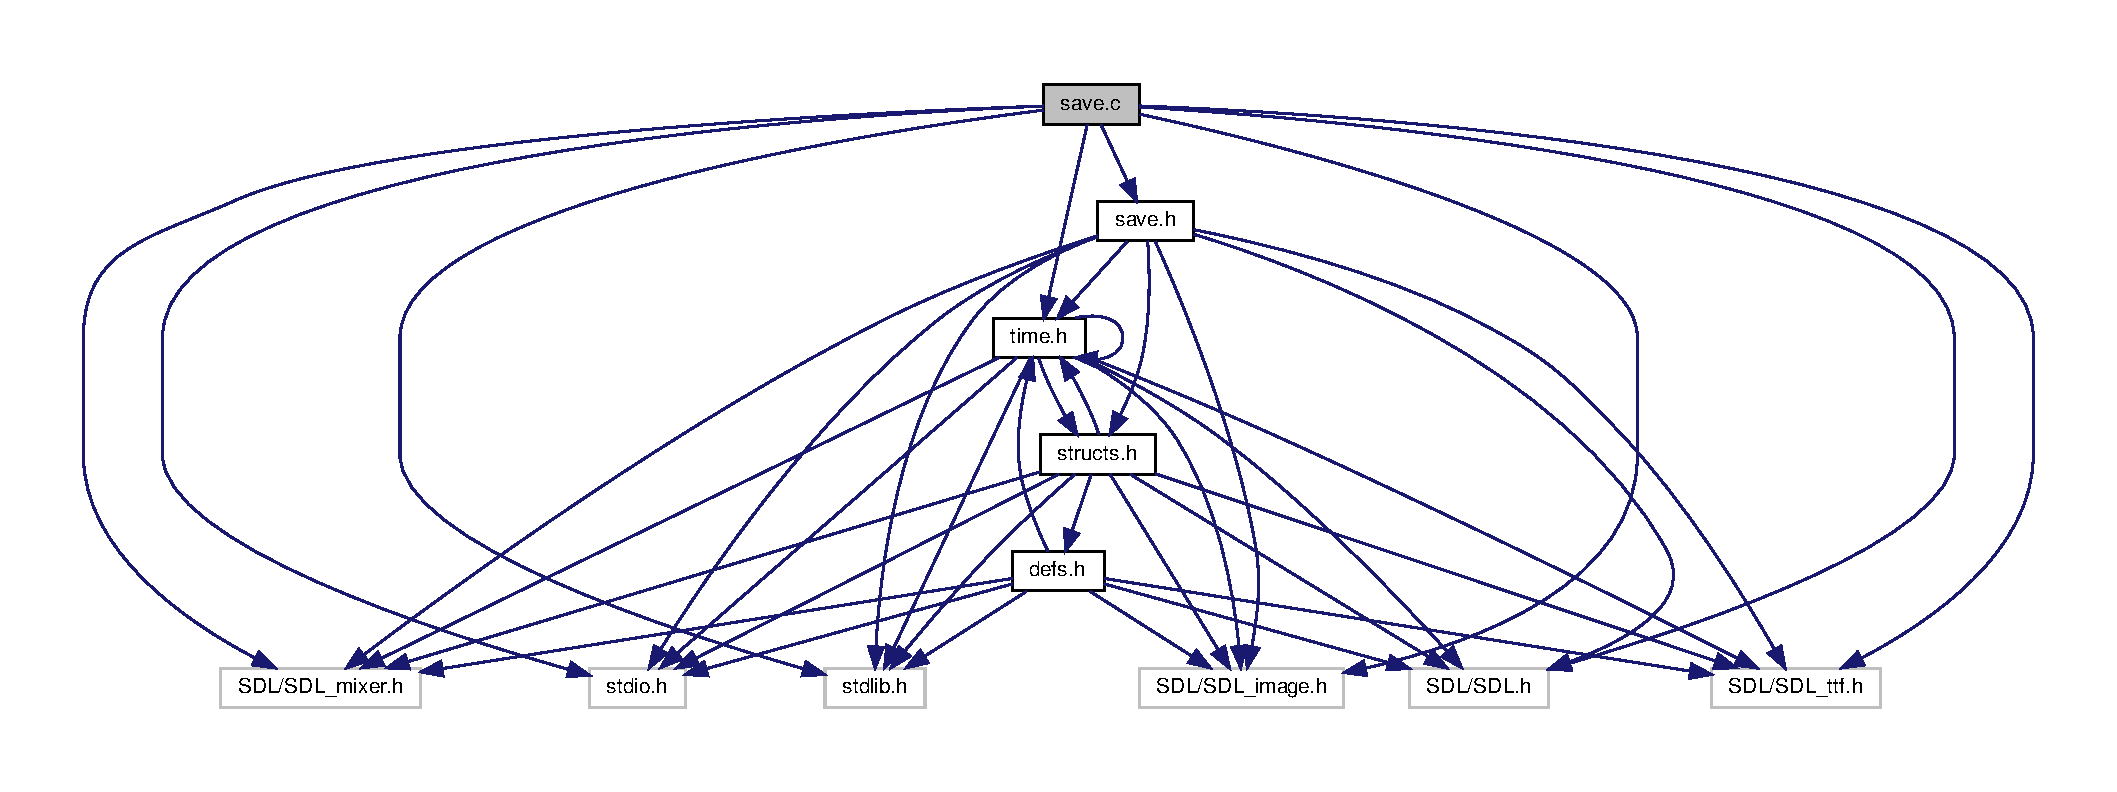
\includegraphics[width=350pt]{save_8c__incl}
\end{center}
\end{figure}
\subsection*{Functions}
\begin{DoxyCompactItemize}
\item 
\mbox{\Hypertarget{save_8c_adadba7f4b031f83e75a7a3b1c6422e51}\label{save_8c_adadba7f4b031f83e75a7a3b1c6422e51}} 
void {\bfseries save} (\hyperlink{structHero}{Hero} player, \hyperlink{structGestion}{Gestion} jeu, \hyperlink{structMap}{Map} map, char nom\+Fich\mbox{[}$\,$\mbox{]})
\item 
\mbox{\Hypertarget{save_8c_a229189c8cd63f8858a396ac7d374202e}\label{save_8c_a229189c8cd63f8858a396ac7d374202e}} 
void {\bfseries load} (\hyperlink{structHero}{Hero} $\ast$player, \hyperlink{structGestion}{Gestion} $\ast$jeu, \hyperlink{structMap}{Map} $\ast$map, char nom\+Fich\mbox{[}$\,$\mbox{]})
\end{DoxyCompactItemize}


\subsection{Detailed Description}
save libs 

\begin{DoxyAuthor}{Author}
Raed 
\end{DoxyAuthor}
\begin{DoxyVersion}{Version}
1.\+0 
\end{DoxyVersion}
\begin{DoxyDate}{Date}
07/06/2020 
\end{DoxyDate}

\hypertarget{save_8h}{}\section{save.\+h File Reference}
\label{save_8h}\index{save.\+h@{save.\+h}}


save libs  


{\ttfamily \#include $<$stdlib.\+h$>$}\newline
{\ttfamily \#include $<$stdio.\+h$>$}\newline
{\ttfamily \#include $<$S\+D\+L/\+S\+D\+L.\+h$>$}\newline
{\ttfamily \#include $<$S\+D\+L/\+S\+D\+L\+\_\+image.\+h$>$}\newline
{\ttfamily \#include $<$S\+D\+L/\+S\+D\+L\+\_\+mixer.\+h$>$}\newline
{\ttfamily \#include $<$S\+D\+L/\+S\+D\+L\+\_\+ttf.\+h$>$}\newline
{\ttfamily \#include $<$time.\+h$>$}\newline
{\ttfamily \#include \char`\"{}structs.\+h\char`\"{}}\newline
Include dependency graph for save.\+h\+:
\nopagebreak
\begin{figure}[H]
\begin{center}
\leavevmode
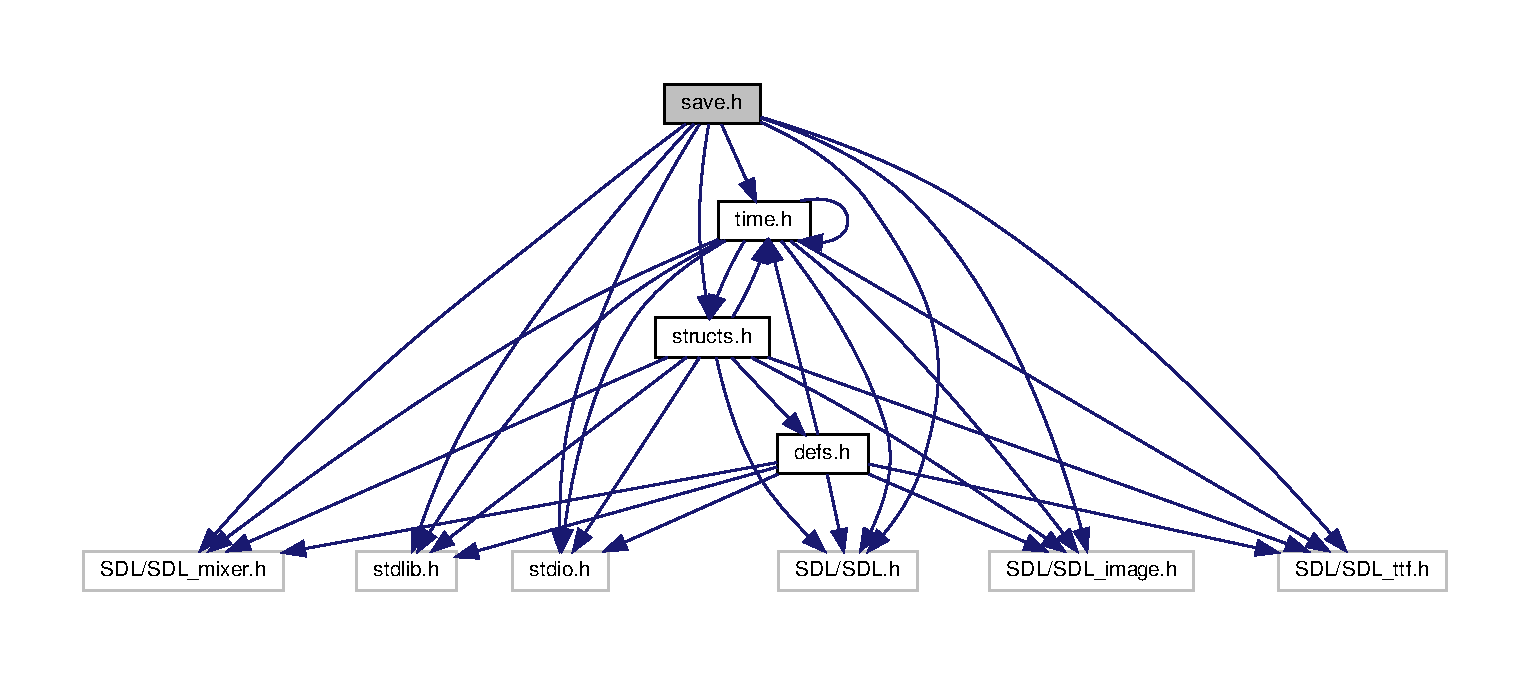
\includegraphics[width=350pt]{save_8h__incl}
\end{center}
\end{figure}
This graph shows which files directly or indirectly include this file\+:
\nopagebreak
\begin{figure}[H]
\begin{center}
\leavevmode
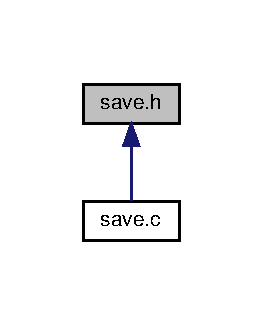
\includegraphics[width=126pt]{save_8h__dep__incl}
\end{center}
\end{figure}
\subsection*{Functions}
\begin{DoxyCompactItemize}
\item 
\mbox{\Hypertarget{save_8h_adadba7f4b031f83e75a7a3b1c6422e51}\label{save_8h_adadba7f4b031f83e75a7a3b1c6422e51}} 
void {\bfseries save} (\hyperlink{structHero}{Hero} player, \hyperlink{structGestion}{Gestion} jeu, \hyperlink{structMap}{Map} map, char nom\+Fich\mbox{[}$\,$\mbox{]})
\item 
\mbox{\Hypertarget{save_8h_a229189c8cd63f8858a396ac7d374202e}\label{save_8h_a229189c8cd63f8858a396ac7d374202e}} 
void {\bfseries load} (\hyperlink{structHero}{Hero} $\ast$player, \hyperlink{structGestion}{Gestion} $\ast$jeu, \hyperlink{structMap}{Map} $\ast$map, char nom\+Fich\mbox{[}$\,$\mbox{]})
\end{DoxyCompactItemize}
\subsection*{Variables}
\begin{DoxyCompactItemize}
\item 
\mbox{\Hypertarget{save_8h_abbeff4ee7b328d6b61b563ecded5bf83}\label{save_8h_abbeff4ee7b328d6b61b563ecded5bf83}} 
\hyperlink{structGestion}{Gestion} {\bfseries jeu}
\item 
\mbox{\Hypertarget{save_8h_a2737dcd286631af70eac9ebd6de78a07}\label{save_8h_a2737dcd286631af70eac9ebd6de78a07}} 
\hyperlink{structHero}{Hero} {\bfseries monster}
\item 
\mbox{\Hypertarget{save_8h_ac9becb8e2f80125547c8cc8f9d56b7ab}\label{save_8h_ac9becb8e2f80125547c8cc8f9d56b7ab}} 
\hyperlink{structMap}{Map} {\bfseries map}
\end{DoxyCompactItemize}


\subsection{Detailed Description}
save libs 

\begin{DoxyAuthor}{Author}
Raed 
\end{DoxyAuthor}
\begin{DoxyVersion}{Version}
1.\+0 
\end{DoxyVersion}
\begin{DoxyDate}{Date}
07/06/2020 
\end{DoxyDate}

\hypertarget{structs_8h}{}\section{structs.\+h File Reference}
\label{structs_8h}\index{structs.\+h@{structs.\+h}}


structs libs  


{\ttfamily \#include $<$stdlib.\+h$>$}\newline
{\ttfamily \#include $<$stdio.\+h$>$}\newline
{\ttfamily \#include $<$S\+D\+L/\+S\+D\+L.\+h$>$}\newline
{\ttfamily \#include $<$S\+D\+L/\+S\+D\+L\+\_\+image.\+h$>$}\newline
{\ttfamily \#include $<$S\+D\+L/\+S\+D\+L\+\_\+mixer.\+h$>$}\newline
{\ttfamily \#include $<$S\+D\+L/\+S\+D\+L\+\_\+ttf.\+h$>$}\newline
{\ttfamily \#include $<$time.\+h$>$}\newline
{\ttfamily \#include \char`\"{}defs.\+h\char`\"{}}\newline
Include dependency graph for structs.\+h\+:
\nopagebreak
\begin{figure}[H]
\begin{center}
\leavevmode
\includegraphics[width=350pt]{structs_8h__incl}
\end{center}
\end{figure}
This graph shows which files directly or indirectly include this file\+:
\nopagebreak
\begin{figure}[H]
\begin{center}
\leavevmode
\includegraphics[width=350pt]{structs_8h__dep__incl}
\end{center}
\end{figure}
\subsection*{Data Structures}
\begin{DoxyCompactItemize}
\item 
struct \hyperlink{structInput}{Input}
\item 
struct \hyperlink{structGestion}{Gestion}
\item 
struct \hyperlink{structMap}{Map}
\item 
struct \hyperlink{structHero}{Hero}
\item 
struct \hyperlink{structGameobject}{Gameobject}
\end{DoxyCompactItemize}
\subsection*{Typedefs}
\begin{DoxyCompactItemize}
\item 
\mbox{\Hypertarget{structs_8h_af2d6a918eb4efb35fbd3a7b1a02bf003}\label{structs_8h_af2d6a918eb4efb35fbd3a7b1a02bf003}} 
typedef struct \hyperlink{structInput}{Input} {\bfseries Input}
\item 
\mbox{\Hypertarget{structs_8h_adf57dcf439abf1fa1b30fec00199edcd}\label{structs_8h_adf57dcf439abf1fa1b30fec00199edcd}} 
typedef struct \hyperlink{structGestion}{Gestion} {\bfseries Gestion}
\item 
\mbox{\Hypertarget{structs_8h_aca840b6acee4aaeed71f7bb576720f84}\label{structs_8h_aca840b6acee4aaeed71f7bb576720f84}} 
typedef struct \hyperlink{structMap}{Map} {\bfseries Map}
\item 
\mbox{\Hypertarget{structs_8h_a6e68f04808182a2df6ec3b64d93ee6d3}\label{structs_8h_a6e68f04808182a2df6ec3b64d93ee6d3}} 
typedef struct \hyperlink{structHero}{Hero} {\bfseries Hero}
\item 
\mbox{\Hypertarget{structs_8h_a833da9c13874c9ae69371a1d03bcfb8b}\label{structs_8h_a833da9c13874c9ae69371a1d03bcfb8b}} 
typedef struct \hyperlink{structGameobject}{Gameobject} {\bfseries Gameobject}
\end{DoxyCompactItemize}


\subsection{Detailed Description}
structs libs 

\begin{DoxyAuthor}{Author}
youssef 
\end{DoxyAuthor}
\begin{DoxyVersion}{Version}
1.\+0 
\end{DoxyVersion}
\begin{DoxyDate}{Date}
07/06/2020 
\end{DoxyDate}

\hypertarget{time_8c}{}\section{time.\+c File Reference}
\label{time_8c}\index{time.\+c@{time.\+c}}


time libs  


{\ttfamily \#include $<$stdlib.\+h$>$}\newline
{\ttfamily \#include $<$stdio.\+h$>$}\newline
{\ttfamily \#include $<$S\+D\+L/\+S\+D\+L.\+h$>$}\newline
{\ttfamily \#include $<$S\+D\+L/\+S\+D\+L\+\_\+image.\+h$>$}\newline
{\ttfamily \#include $<$S\+D\+L/\+S\+D\+L\+\_\+mixer.\+h$>$}\newline
{\ttfamily \#include $<$S\+D\+L/\+S\+D\+L\+\_\+ttf.\+h$>$}\newline
{\ttfamily \#include $<$time.\+h$>$}\newline
Include dependency graph for time.\+c\+:
\nopagebreak
\begin{figure}[H]
\begin{center}
\leavevmode
\includegraphics[width=350pt]{time_8c__incl}
\end{center}
\end{figure}
\subsection*{Functions}
\begin{DoxyCompactItemize}
\item 
\mbox{\Hypertarget{time_8c_a3c3e683a005eace2dd1e4d551056d9b6}\label{time_8c_a3c3e683a005eace2dd1e4d551056d9b6}} 
void {\bfseries timer} ()
\end{DoxyCompactItemize}


\subsection{Detailed Description}
time libs 

\begin{DoxyAuthor}{Author}
Raed 
\end{DoxyAuthor}
\begin{DoxyVersion}{Version}
1.\+0 
\end{DoxyVersion}
\begin{DoxyDate}{Date}
07/06/2020 
\end{DoxyDate}

\hypertarget{time_8h}{}\section{time.\+h File Reference}
\label{time_8h}\index{time.\+h@{time.\+h}}


time libs  


{\ttfamily \#include $<$stdlib.\+h$>$}\newline
{\ttfamily \#include $<$stdio.\+h$>$}\newline
{\ttfamily \#include $<$S\+D\+L/\+S\+D\+L.\+h$>$}\newline
{\ttfamily \#include $<$S\+D\+L/\+S\+D\+L\+\_\+image.\+h$>$}\newline
{\ttfamily \#include $<$S\+D\+L/\+S\+D\+L\+\_\+mixer.\+h$>$}\newline
{\ttfamily \#include $<$S\+D\+L/\+S\+D\+L\+\_\+ttf.\+h$>$}\newline
{\ttfamily \#include $<$time.\+h$>$}\newline
{\ttfamily \#include \char`\"{}structs.\+h\char`\"{}}\newline
Include dependency graph for time.\+h\+:
\nopagebreak
\begin{figure}[H]
\begin{center}
\leavevmode
\includegraphics[width=350pt]{time_8h__incl}
\end{center}
\end{figure}
This graph shows which files directly or indirectly include this file\+:
\nopagebreak
\begin{figure}[H]
\begin{center}
\leavevmode
\includegraphics[width=350pt]{time_8h__dep__incl}
\end{center}
\end{figure}
\subsection*{Functions}
\begin{DoxyCompactItemize}
\item 
\mbox{\Hypertarget{time_8h_a3c3e683a005eace2dd1e4d551056d9b6}\label{time_8h_a3c3e683a005eace2dd1e4d551056d9b6}} 
void {\bfseries timer} ()
\end{DoxyCompactItemize}
\subsection*{Variables}
\begin{DoxyCompactItemize}
\item 
\mbox{\Hypertarget{time_8h_abbeff4ee7b328d6b61b563ecded5bf83}\label{time_8h_abbeff4ee7b328d6b61b563ecded5bf83}} 
\hyperlink{structGestion}{Gestion} {\bfseries jeu}
\end{DoxyCompactItemize}


\subsection{Detailed Description}
time libs 

\begin{DoxyAuthor}{Author}
Raed 
\end{DoxyAuthor}
\begin{DoxyVersion}{Version}
1.\+0 
\end{DoxyVersion}
\begin{DoxyDate}{Date}
07/06/2020 
\end{DoxyDate}

%--- End generated contents ---

% Index
\backmatter
\newpage
\phantomsection
\clearemptydoublepage
\addcontentsline{toc}{chapter}{Index}
\printindex

\end{document}
